%%
%% memoria.tex
%% 
%\documentclass[a4paper,12pt,titlepage,halfparskip, cleardoubleempty]{scrbook}
\documentclass[a4paper,12pt]{scrbook}
\pagestyle{headings}

% Referencias externas
\usepackage{xr-hyper}

%\usepackage[pdftex, breaklinks=false]{hyperref}
\usepackage[pdftex, breaklinks=false, colorlinks=true, linkcolor=black, anchorcolor=black, urlcolor=blue, citecolor=red]{hyperref}

\usepackage[T1]{fontenc}
\usepackage[spanish]{babel}
\usepackage[utf8]{inputenc}

\usepackage[printonlyused]{acronym-custom}

\usepackage{inconsolata}

%\usepackage{titlesec}



%%%%%%%%%%%%%%%
% Paquetes para fuentes

% Paquete para la fuente charter
\usepackage{charter}

% Paquete para la fuente helvética
\usepackage[scaled=0.92]{helvet}

% Paquete para la fuente Courier
% \usepackage{courier}

\usepackage{gnuplottex}

% Guiones de hyphenado
\usepackage{hyphenat}

% Paquete para hacer un índice
\usepackage{makeidx}

% Extra ToC listings
\usepackage{tocbibind}

% Gráficos
\usepackage{graphicx}

% Extensión para el entorno enumerate ¿?
%\usepackage{enumerate}

% Para poner figuras una al lado de otra
\usepackage[lofdepth,lotdepth]{subfig}

% Paquete para figuras giradas
\usepackage{rotating}

% Paquete de matemáticas
%\usepackage{amstext}

% Define el entorno altt, como un verbatim pero se pueden utilizar fórmulas matemáticas
%\usepackage{alltt}

% Listados de código
%\usepackage{listings}

% Herramientas para alinear las comas decimales en columnas en un entorno tabular o array
%\usepackage{dcolumn}
%\usepackage{array}

% Extensión para el entorno tabular
%\usepackage{tabularx}

% Entornos wrapfigure y wraptable para poner texto alrededor de figuras
%\usepackage{wrapfig}

% Automatiza el resaltado de sintaxis usando pygments
\usepackage{minted}

\addto\captionsspanish{
\renewcommand\bibname{Bibliografía y referencias}
}

\makeindex

\begin{document}


%% PRODUCTOS
\newcommand{\nombrepostprocesador}{ACL2:\colonhyp{}Procesador}
\newcommand{\nombrevisor}{XMLEye}
\newcommand{\nombreyaxml}{YAXML:\colonhyp{}Reverse}
\newcommand{\postprocesador}{\texttt{\nombrepostprocesador}\xspace}
\newcommand{\visor}{\nombrevisor\xspace}
\newcommand{\yaxml}{\texttt{\nombreyaxml}\xspace}

\newcommand{\biblioteca}[1]{\index{#1}\texttt{#1}}

% YAML/YAXML
\newcommand{\etiqueta}[1]{{\bfseries \ttfamily #1}}

% ACL2

\newcommand{\orden}[1]{\texttt{#1}}   % Nombre de orden ACL2
\newcommand{\fichero}[1]{\texttt{#1}} % Nombre de fichero
\newcommand{\evento}[1]{\texttt{#1}}  % Nombre de un evento
\newcommand{\lisp}[1]{\textit{#1}}    % Trozo de c�digo Lisp
\newcommand{\libro}[1]{\textsc{#1}}   % Libro ACL2

% PERL

\newcommand{\modulo}[1]{\index{m�dulo Perl!#1}\index{#1|see{m�dulo Perl!#1}}\texttt{#1}}
\newcommand{\funcion}[1]{\textit{#1}}

% JAVA

\newcommand{\clase}[1]{\textit{#1}}   % Clase Java
\newcommand{\metodo}[1]{\texttt{#1}}  % M�todo (tambi�n Perl)
\newcommand{\paquete}[1]{\texttt{#1}}

%% MANUALES

\newcommand{\accesoteclado}[1]{\textsc{#1}} % Acceso de teclado

%% OTROS

\newcommand{\patron}[1]{\emph{#1}}

\newcolumntype{,}{>{$}r<{$}}
\newcommand{\Index}[1]{#1\emph{\index{#1}}}

\newcounter{pasoacept}

\newenvironment{pruebaaceptacion}{
  \setcounter{pasoacept}{0}
  \begin{center}
  \begin{tabular}{| >{\stepcounter{pasoacept}\arabic{pasoacept}. }p{.4\linewidth} | p{.5\linewidth}|}
    \hline
    \multicolumn{1}{| c |}{\textbf{Paso seguido}} & \multicolumn{1}{c|}{\textbf{Resultado esperado}} \\
    \hline
    \hline
}{
  \hline
  \end{tabular}
  \end{center}
}

% http://www.tex.ac.uk/cgi-bin/texfaq2html?label=chngmargonfly

\newenvironment{changemargin}[2]{%
  \begin{list}{}{%
    \setlength{\topsep}{0pt}%
    \setlength{\leftmargin}{#1}%
    \setlength{\rightmargin}{#2}%
    \setlength{\listparindent}{\parindent}%
    \setlength{\itemindent}{\parindent}%
    \setlength{\parsep}{\parskip}%
  }%
  \item[]}{\end{list}}

\newenvironment{nota}{
  \begin{changemargin}{2em}{2em}
    \textbf{\textsc{Nota: }}
}{
  \end{changemargin}
}

\renewcommand{\lstlistlistingname}{Listados}
\renewcommand{\lstlistingname}{Listado}

\newcommand{\CPP}
{\mbox{C\hspace{-.1em}\raise.2ex\hbox{+\hspace{-.1em}+}}\xspace}

\setlength{\extrarowheight}{4pt}

\lstset{
  extendedchars,
  flexiblecolumns,
  stringstyle=\ttfamily,
  showstringspaces=false,
  frame=tb
}

%% PARTE DE DOCBOOK

\newcommand{\application}[1]{\index{#1}\emph{#1}}
\newcommand{\cmdsynopsis}[1]{\nohyphens{\texttt{#1}}}
\newcommand*{\command}[1]{\nohyphens{\textbf{\texttt{#1}}}}
\newcommand{\constant}[1]{\texttt{#1}}
\newcommand{\computeroutput}[1]{#1}
\newcommand*{\email}[1]{\nohyphens{\texttt{#1}}}
\newcommand*{\envar}[1]{\nohyphens{\texttt{#1}}}
\newcommand*{\filename}[1]{\texttt{#1}}
\newcommand*{\guibutton}[2][]{\emph{#2}}
\newcommand*{\guilabel}[2][]{\emph{#2}}
\newcommand*{\guimenuitem}[2][]{\emph{#2}}
\newcommand*{\guimenu}[2][]{\emph{#2}}
\newcommand*{\keycombo}[1]{\textsc{#1}}
\newcommand*{\keysym}[1]{\textsc{#1}}
\newcommand*{\option}[1]{\nohyphens{\texttt{#1}}}
\newcommand{\prompt}[1]{#1}
\newcommand{\varname}[1]{\nohyphens{\texttt{#1}}}

\newcommand{\note}[1]{\vskip 1em
    \fbox{\parbox{\textwidth}{\textsc{Nota}
    \vskip 1em #1}} \vskip 1em}


%%% Local Variables: 
%%% mode: latex
%%% TeX-master: "memoria"
%%% End: 


% Portada
\begin{titlepage}
  \centering
  
\includegraphics[width=.3\textwidth]{logo_uca}

  \bigskip
  \bigskip
  \bigskip
  
%  \begin{changemargin}{3em}{3em}
    \centering

    {\Huge \textsc{\nohyphens{Escuela Superior de Ingeniería}}}
    
    \bigskip
    \bigskip
    \bigskip

    {\huge \nohyphens{Ingeniería Técnica en Informática de Sistemas}}

    \bigskip
    \bigskip
    \bigskip
    \bigskip
    \bigskip
    \bigskip

    {\LARGE \nohyphens{oFlute}}

    \bigskip
    \bigskip
    \bigskip
    \bigskip

    {\large Curso 2009-2010}

    \bigskip
    \bigskip
    \bigskip
    \bigskip
    \bigskip
    \bigskip
    \bigskip
      
%  \end{changemargin}

  {\Large José Tomás Tocino García \\}
  {\large Cádiz, \today}

\end{titlepage}

\cleardoublepage

% Segunda portada
{
  \thispagestyle{empty}
  \centering
  
\includegraphics[width=.2\textwidth]{logo_uca}

  \bigskip
  \bigskip
  \bigskip
  
  \begin{changemargin}{3em}{3em}

    \begin{center}
      {\Huge \textsc{\nohyphens{Escuela Superior de Ingeniería}}}
      
      \bigskip
      \bigskip
      
      {\huge \nohyphens{Ingeniería Técnica en Informática de Sistemas}}
      
      \bigskip
      \bigskip
      \bigskip
      \bigskip
      
      {\LARGE \nohyphens{oFlute}}
      
      \bigskip
      \bigskip
      \bigskip
      \bigskip
      
    \end{center}
  \end{changemargin}
  \begin{changemargin}{3em}{1em}
  \begin{flushleft}
    \Large

    \textsc{Departamento}: \nohyphens{Lenguajes y Sistemas Informáticos.} \\
    \textsc{Director del proyecto}: \nohyphens{Manuel Palomo Duarte.} \\
    \textsc{Autor del Proyecto}: \nohyphens{José Tomás Tocino García}. \\
  \end{flushleft}

  \end{changemargin}  

  \bigskip
  \bigskip
  \bigskip
  
  \begin{flushright}
    \large
    Cádiz, \today
    
    Fdo.: José Tomás Tocino García
    
  \end{flushright}

}


\cleardoublepage
\bigskip
\bigskip

Este documento se halla bajo la licencia \ac{FDL}. Según estipula la
licencia, se muestra aquí el aviso de copyright. Se ha usado la
versión inglesa de la licencia, al ser la única reconocida
oficialmente por la \ac{FSF}.

\begin{quote}
  Copyright \copyright  2010 José Tomás Tocino García.
  
  Permission is granted to copy, distribute and/or modify this document
  under the terms of the GNU Free Documentation License, Version 1.2
  or any later version published by the Free Software Foundation;
  with no Invariant Sections, no Front-Cover Texts, and no Back-Cover Texts.
  A copy of the license is included in the section entitled "GNU
  Free Documentation License".
\end{quote}

\cleardoublepage

\section*{Agradecimientos}

A Julian Raschke por crear y mantener Gosu.

\cleardoublepage

\tableofcontents
\listoffigures
%\listoftables

\setlength{\parskip}{1.2ex plus 0.4ex minus 0.1ex}

\chapter{Introducción}
\section{Contexto y motivación}
Las nuevas tecnologías van filtrándose gradualmente en los centros
educativos, y las técnicas de enseñanza se están adaptando a las
opciones que ofrecen. El reparto de ordenadores portátiles a los
alumnos andaluces de 5º y 6º de primaria, dentro del marco de la
Escuela TIC 2.0, es buena muestra de ello. 

Por otro lado, las nuevas generaciones están en plena simbiosis con
las tecnologías de la información, cada vez más acostumbradas al
empleo de dispositivos electrónicos, y su uso ya les es prácticamente
instintivo. Por tanto, es beneficioso buscar nuevos métodos educativos
que hagan uso de las nuevas tecnologías.

En la búsqueda de materias educativas en las que aplicar el uso de las
nuevas tecnologías, la música, parte fundamental del programa
curricular en la educación primaria, ofrece una gran variedad de
aspectos que podrían desarrollarse utilizando tecnologías de la
información. Es ahí donde este proyecto hace su aportación.

\section{Objetivos}
A la hora de definir los objetivos de un sistema, podemos agruparlos
en dos tipos diferentes: \textbf{funcionales} y
\textbf{transversales}. Los primeros se refieren a \textit{qué} debe
hacer la aplicación que vamos a desarrollar, e inciden
directamente en la experiencia del usuario y de potenciales
desarrolladores.

Por otro lado, los objetivos transversales son aquellos invisibles al
usuario final, pero que de forma inherente actúan sobre el resultado
final de la aplicación y sobre la experiencia de desarrollo de la misma.

\subsection{Funcionales}
\begin{itemize}
\item Crear un módulo de análisis del sonido en el dominio de la
  frecuencia para poder identificar las notas capturadas por el
  micrófono en tiempo real.
\item Crear una aplicación de usuario que identifique y muestre en
  pantalla las notas que toca el usuario en cada momento.
\item Reutilizar el módulo de análisis en un juego en el que el
  usuario debe tocar correctamente las notas que aparecen en pantalla
  siguiendo un pentagrama.
\item Incluir un sistema de lecciones multimedia individuales que
  sirvan al alumno de referencia y fuente de aprendizaje.
\item Potenciar el uso de interfaces de usuario amigables, con un
  sistema avanzado de animaciones que proporcione un aspecto fluido y
  evite saltos bruscos entre secciones.
\end{itemize}

\subsection{Transversales}
\begin{itemize}
\item Obtener una base teórica sobre cómo se representa y caracteriza
  digitalmente el sonido.
\item Conocer las bases del \ac{DSP}, y su uso en aplicaciones de
  reconocimiento básico de sonidos, tales como sintonizadores y
  afinadores de instrumentos.
\item Introducirme en la programación de audio en sistemas GNU/Linux.
\item Entender las bases del análisis de sonidos en el dominio de la
  frecuencia. 
\item Utilizar un enfoque de análisis, diseño y codificación orientado
  a objetos, de una forma lo más clara y modular posible, para
  permitir ampliaciones y modificaciones sobre la aplicación por
  terceras personas.
\item Hacer uso de herramientas básicas en el desarrollo de software,
  como son los \textbf{Sistemas de Control de Versiones} para llevar
  un control realista del desarrollo del software, así como hacer de
  las veces de sistema de copias de seguridad.
\end{itemize}


\section{Alcance}
\textbf{oFlute} se modela como una herramienta lúdico-educativa para
alumnos que comiencen a aprender a usar la flauta dulce,
proporcionando un entorno atractivo y ameno para el estudiante. Éstos
tendrán la posibilidad de recorrer una serie de pequeñas lecciones
sobre música en general, y el uso de la flauta dulce en particular.

Además, el usuario tendrá la posibilidad de comprobar sus
conocimientos sobre el uso de la flauta practicando, gracias a las
secciones de análisis de notas y de canciones, en las que la
aplicación valorará la pericia del estudiante con la flauta.  

\subsection{Limitaciones del proyecto}
El proyecto se limita al uso de la flauta dulce y no a otros
instrumentos por la enorme variabilidad de timbre entre ellos, lo que
supondría un enorme esfuerzo a la hora de generalizar el analizador de
frecuencias.

El sistema de lecciones se basa en plantillas XML en las que es
posible definir imágenes y texto para formar una pantalla
de información. En un futuro se ampliará para incluir otros elementos
multimedia así como lecciones con varias pantallas consecutivas.

Los sistemas de audio son una de las áreas en las que menos consenso hay entre
plataformas informáticas, por lo que la transportabilidad de las aplicaciones
suele ser compleja. El presente proyecto utiliza la API Simple de PulseAudio
como subsistema de sonido, que es en teoría compatible con plataformas Win32,
pero en la práctica su complejidad hace prácticamente inviable la portabilidad
de la aplicación.

\subsection{Licencia}
El proyecto está publicado como software libre bajo la licencia
\ac{GPL} versión 2. El conjunto de bibliotecas y módulos utilizados
tienen las siguientes licencias:
\begin{itemize}

\item A lo largo del proyecto se utilizan diferentes partes de las
  bibliotecas \textbf{Boost}~\cite{boost}, que utilizan la licencia
  \textit{Boost Software License}~\footnote{\url{http://www.boost.org/LICENSE_1_0.txt}}.
  Se trata de una licencia de software libre, compatible con la GPL, y
  comparable en permisividad a las licencias BSD y MIT.

\item \textbf{Gosu}~\cite{gosu}, la biblioteca de desarrollo de
  videojuegos que ha proporcionado el subsistema gráfico, utiliza la
  licencia \ac{MIT}. Cuando se compila en sistemas Windows, utiliza la
  biblioteca FMOD que es gratuita pero de código cerrado; en sistemas
  GNU/Linux, utiliza SDL\_mixer, que utiliza la licencia \ac{LGPL}.

\item \textbf{Kiss FFT}~\cite{kissfft}, la biblioteca utilizada para
  hacer el análisis de frecuencias, utiliza una licencia \ac{BSD}.

\item \textbf{PugiXML}~\cite{pugixml}, biblioteca de procesamiento de
  ficheros XML, se distribuye bajo al licencia MIT.

\item \textbf{PulseAudio}~\cite{pulseaudio} utiliza una licencia LGPL 2.1.
\end{itemize}

\section{Estructura del documento}
El presente documento se rige según la siguiente estructura:

\begin{itemize}
\item \textbf{Introducción}. Se exponen las motivaciones y objetivos detrás del
  proyecto \textbf{oFlute}, así como información sobre las licencias de sus
  componentes, glosario y estructura del documento.
\item \textbf{Desarrollo del calendario}, donde se explica la planificación del
  proyecto, la división de sus etapas, la extensión de las etapas a lo largo del
  tiempo y los porcentajes de esfuerzo.
\item \textbf{Investigación preliminar}, que explica las labores de
  documentación y experimentación previas al desarrollo, que han servido para
  labrar una base de conocimientos que nos diera las suficientes garantías para
  afrontar el proyecto.
\item \textbf{Análisis}. Se detalla la fase de análisis del sistema, explicando
  los requisitos funcionales del sistema, los diferentes casos de uso, así como
  las principales operaciones con sus diagramas de secuencia y contratos.
\item \textbf{Diseño}. Seguido del análisis, se expone en detalle la etapa de
  diseño del sistema, con los diagramas de clases.
\item \textbf{Implementación}. Una vez analizado el sistema y definido su
  diseño, en esta parte se detallan las decisiones de implementación más
  relevantes que tuvieron lugar durante el desarrollo del proyecto.
\item \textbf{Pruebas}. Listamos y describimos las pruebas que se han llevado a
  cabo sobre el proyecto para garantizar su fiabilidad y consistencia.
\marginpar{RELLENAR}
\end{itemize}

Tras una revisión del calendario seguido, detallaremos a lo largo del
resto de la memoria el proceso de análisis, diseño, codificación y
pruebas que se siguió al realizar el proyecto.  

Los manuales de usuario y de instalación se incluyen tras un resumen
de los aspectos más destacables de proyecto y las conclusiones. En
dicho manual, se hallan dos apartados dirigidos a la ampliación de la
aplicación mediante la creación de nuevas lecciones y de nuevas
canciones, respectivamente.



\chapter{Desarrollo del calendario}
\label{chap:calendario}
El proyecto no se ha desarrollado siguiendo un calendario estricto,
dado que era imposible cuantificar el tiempo que tomaría el adquirir
las bases teóricas necesarias para poder afrontarlo con garantías. Su
desarrollo se ha compaginado con los estudios del último curso de
Ingeniería Técnica en Informática de Sistemas y las labores como
becario en la Oficina de Software Libre y Conocimiento Abierto de la
Universidad de Cádiz~\cite{osluca}.

\section{Iteraciones}

Para la realización del presente proyecto se ha utilizado un modelo de
desarrollo iterativo incremental. A continuación se detallan cada una
de las etapas por las que ha ido pasando el software, y se observará
como conforme se iba avanzando se añadían nuevas funcionalidades y se
pulían las existentes.

\section{Diagrama de Gantt}

\section{Porcentajes de esfuerzo}



%\chapter{Descripción general del proyecto}
%
\section{Perspectiva del producto}

\section{Funciones}

Lista de funciones

\section{Características de los usuarios}

\section{Restricciones generales}

\section{Suposiciones y dependencias}


\section{Requisitos para futuras versiones}








 
\chapter{Investigación preliminar}
\section{Adquisición de conocimientos}
Para poder enfrentarnos con garantías al desarrollo del proyecto fue necesario
adquirir una \textbf{base de conocimientos} que nos permitiera entender los
conceptos que se iban a usar y las herramientas para trabajar con ellos. Así,
fuimos guiándonos por la intuición y, sobre todo, por las necesidades que iban
surgiendo. 

Los conceptos que se presentan a continuación son básicos para comprender cómo
funciona el módulo de análisis del proyecto.

\subsection{El sonido}
Un \textbf{sonido} es una vibración que se propaga por un medio
elástico en forma de onda. Estas vibraciones se transmiten de forma
longitudinal, esto es, en la misma dirección en la que se propaga la
onda. El medio más común para la transmisión del sonido es el
\textbf{aire}. 

El sonido, en su forma más simple, se compone de una sola onda
sinusoidal básica, con las características tradicionales: amplitud,
frecuencia y fase. Una \textbf{onda sinusoidal} es aquella cuyos
valores se calculan utilizando funciones seno.

\subsubsection{Frecuencia y tono}
La \textbf{frecuencia} mide el número de oscilaciones de la onda por
unidad de tiempo. Por regla general, se utiliza el \textbf{hercio}
como unidad de medida de frecuencia, que indica la cantidad de
repeticiones por segundo. La frecuencia determinará la \textbf{altura}
del sonido, es decir, cómo de grave o agudo es. Los sonidos graves
tienen una frecuencia baja, mientras que los sonidos agudos tienen una
frecuencia alta.

A lo largo de los años se ha establecido un estándar de referencia que
establece que la nota \textit{la} que se encuentra encima del
\textit{do} central del piano debe sonar a 440 hercios de
frecuencia. Esta medida se utiliza a la hora de afinar los
instrumentos, de modo que si al tocar la nota \textit{la} se detecta
un tono con una frecuencia de 440 hercios, entonces el instrumento
estará bien afinado.

El espectro audible por las personas lo conforman las
\textbf{audiofrecuencias}, esto es, el conjunto de frecuencias que
pueden ser percibidas por el oído humano. 

\begin{figure}[h]
  \centering
  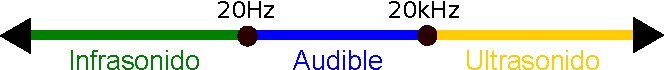
\includegraphics[scale=0.8]{3_investigacion/imagen_rango_frecuencias}
  \caption{Rango de frecuencias de sonido}
\end{figure}


Un oído sano y joven es capaz de detectar sonidos a partir de los 20
hercios. Los sonidos por debajo de esa frecuencia se conocen como
\textbf{infrasonidos}. Por otro lado, el límite auditivo en
frecuencias altas varía mucho con la edad: un adolescente puede oir
sonidos con frecuencias hasta los 18kHz, mientras que un adulto de
edad media solo suele llegar a captar sonidos de hasta 13kHz. El
límite genérico superior se establece en 20kHz, por encima de los
cuales los sonidos se denominan \textbf{ultrasonidos}.


\subsubsection{Amplitud}
La \textbf{amplitud} representa la energía que transporta la
onda. Cuando un instrumento u otro objeto genera una vibración, la
amplitud es la cantidad de movimiento que esa vibración genera.
Podría equipararse (de forma no estricta) a la intensidad del sonido:
cuanto mayor sea la amplitud, más fuerte se oirá el sonido.

\subsubsection{Fase}
Por último, la \textbf{fase} ($\varphi$) indica el desplazamiento
horizontal de la onda respecto del origen. Si la fase de una onda no
es cero, entonces parecerá que está \textit{desplazada} hacia la
derecha, si la fase es positiva, y hacia la izquierda si la fase es
negativa.
\begin{figure}[h]\centering
    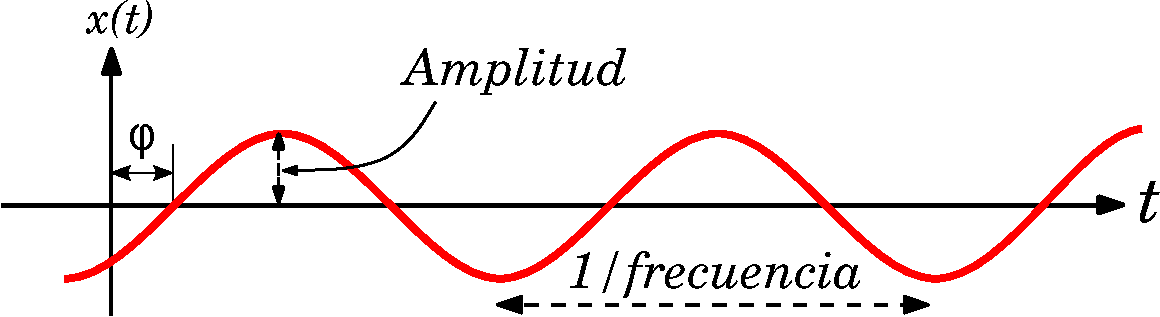
\includegraphics[scale=0.7]{3_investigacion/imagen_onda}
    \caption{Componentes de una señal senoidal básica}
\end{figure}
\subsection{Descomposición de sonidos}
Para desarrollar oFlute nos interesa conocer la altura de la nota que
está tocando la flauta en un instante concreto. Para un tono puro,
podríamos conocer la altura fijándonos en su frecuencia. El problema
es que, en la naturaleza, \textbf{no existen} los tonos puros, sino
que los sonidos se componen de multitud de tonos de diferentes
amplitudes, frecuencias y fases. 

Afortunadamente, la teoría dicta que cualquier tono complejo puede
descomponerse como suma de tonos puros de distintas amplitudes, fases
y frecuencias, llamados \textbf{parciales}. La menor de todas las
frecuencias de los parciales se conoce como \textbf{frecuencia
  fundamental}, y es la que que dicta la altura general del sonido --
\textit{general}, ya que aunque el resto de frecuencias puede
corresponder a otras notas, es la altura de la frecuencia fundamental
la que mayor relevancia tiene en el sonido.

Un subconjunto de esos parciales, conocidos como \textbf{armónicos},
tienen frecuencias múltiplos de la frecuencia fundamental. Estos
armónicos sirven para enriquecer el sonido y, sobre todo, determinar
el \textbf{timbre musical} del origen del sonido: dos instrumentos (o
personas) pueden estar tocando la misma nota y emitir la misma
frecuencia fundamental, pero será el conjunto total de armónicos el
que nos ayude a distinguir qué instrumento está emitiendo el sonido.

Así pues, el objetivo es encontrar una forma de descomponer una señal
(el sonido) en sus componentes y analizar sus frecuencias, buscando la
frecuencia fundamental, que nos informará de la nota que se está tocando. 

\subsubsection{Representación gráfica de sonidos}

Las representación habitual de las señales se hace en el
\textbf{dominio del tiempo}, es decir, podemos observar cómo la señal
cambia a lo largo del tiempo, viendo el valor de su \textbf{amplitud}
en cada instante. Por otro lado, la representación en el
\textbf{dominio de la frecuencia} nos permite analizar una señal
respecto a las frecuencias que la componen, dividiendo la señal en sus
componentes.

En la figura \ref{fig:wavespectral} podemos comparar la representación de
un sonido en el dominio del tiempo, en \textbf{forma de ondas}, tal y
como aparecería en un osciloscopio, frente a su representación en
\textbf{forma espectral}, en la que el eje vertical indica la
frecuencia, y la intensidad del color indica la intensidad de esa
componente frecuencial en el sonido.

\begin{figure}[h!]
  \centering
  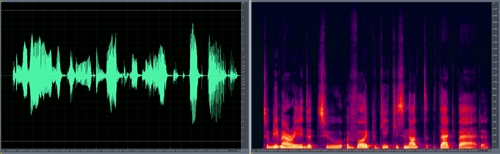
\includegraphics[scale=0.8]{3_investigacion/imagen_forma_espectral}
  \caption{Forma de ondas vs representación espectral}
  \label{fig:wavespectral}
\end{figure}

\subsubsection{Herramientas de descomposición de señales}
\label{sec:fourier}
La herramienta fundamental a la hora de descomponer una señal periódica, como
puede ser un sonido, en sus parciales o armónicos es el \textbf{análisis
  armónico} o \textbf{análisis de Fourier}. Esta rama del análisis matemático
estudia la representación de funciones o señales como superposición de ondas
básicas, y hoy en día se aplica en innumerables campos de la ciencia, desde el
procesamiento de señales para el reconocimiento de patrones, como es nuestro
caso, a la neurociencia.

Una de las herramientas más conocidas de este área es la \textbf{transformada de
  Fourier}. Se trata de una aplicación matemática que descompone una función en
su espectro de frecuencias a lo largo del dominio. Al aplicarla sobre una
función $f$, se define de la siguiente manera:

\[
g(\xi ) = \frac{1}{\sqrt{2\pi}} \int_{-\infty}^{+\infty} f(x)e^{-i\xi\,x} dx
\]

De cualquier modo, al estar tratando con un sistema digital como es una
computadora, no es viable aplicar esta definición de la transformada de Fourier,
ya que se basa en funciones continuas y derivables, y en nuestro caso
dispondremos de datos discretos.

De ahí, aparece la \textbf{transformada discreta de Fourier} o \textbf{DFT}, que
tiene el mismo uso que la transformada tradicional pero requiere que la función
de entrada sea una secuencia discreta y de duración finita.

Existe un gran número de aproximaciones al cálculo de la transformada de
Fourier, pero claramente el algoritmo más utilizado y eficiente es el
\textbf{FFT}, \textbf{Fast Fourier Transform}. A pesar de imponer algunas
limitaciones para mantener la eficiencia, el algoritmo FFT es la implementación
que más habitualmente se encuentra en los chips DSP. Por regla general, computar
la transformada de Fourier para $N$ puntos usando FFT tardaría un tiempo $O(N
\cdot log(N))$, mientras que hacerlo utilizando la definición estándar de la DFT
llevaría un tiempo $O(N^2)$.

A pesar de que fue el \textbf{DFT} el algoritmo que se utilizó finalmente en el
proyecto, se estudiaron otras posibles herramientas para la detección de la
frecuencia fundamental, como por ejemplo la \textbf{función de autocorelación},
que también suele utilizarse en análisis de señales para encontrar patrones
repetitivos, como señales enmascaradas por ruido. A pesar de ello, dada la poca
bibliografía encontrada sobre estas técnicas secundarias y la conocida
eficiencia de la transformada de Fourier, se decidió optar por la técnica más
conocida.

\subsection{Digitalización de sonidos}

Antes de poder aplicar ninguna técnica sobre los sonidos, es necesario
transformarlos de forma que el ordenador pueda trabajar con ellos.

\subsubsection{Captación de sonidos}
Lo más habitual a la hora de digitalizar un sonido es, primeramente, utilizar
algún dispositivo que transforme las ondas sonoras en algo que pueda
transmitirse al computador en forma de ondas eléctricas. Este dispositivo es el
\textbf{micrófono}, en nuestro caso de tipo \textbf{electret}, que es el más
utilizado en ordenadores personales, teléfonos móviles y demás dispositivos de
consumo con requisitos de audio de media o baja fidelidad.

Estos micrófonos constan de una membrana que vibra libremente cuando capta
cualquier onda acústica o de sonido, ya sea voz, música o ruidos, convirtiéndola
en una señal eléctrica de baja frecuencia y de muy poca tensión o voltaje,
semejante a la del sonido captado. Una vez que esta señal eléctrica llega a la
tarjeta de sonido, comienza la siguiente parte del proceso.

Curiosamente, el proceso es el inverso del que ocurre en un altavoz. Es por eso
que en el caso de algunos auriculares intrauditivos, como los que habitualmente
acompañan a los reproductores MP3 de bolsillo, es posible utilizarlos como
micrófonos de baja fidelidad. También es posible, aunque bastante más difícil,
utilizar ciertos micrófonos de escritorio como altavoces improvisados, limitados
a la reproducción de altas frecuencias.

\subsubsection{Muestreo de la señal}
\label{sec:nyquist}
El siguiente paso es el \textbf{muestreo} (o \textit{sampling}) de la señal. El
proceso consiste en medir la amplitud de la señal analógica en diferentes
puntos, uniformemente espaciados, a lo largo del tiempo. El número de veces que
se muestrea la señal por unidad de tiempo es conocido como \textbf{frecuencia de
  muestreo}, e influye directamente en la calidad de la digitalización del sonido.

La elección de la frecuencia de muestreo no suele ser trivial y tiene un impacto
importante en el rendimiento y calidad del sistema, ya que el número de
elementos a procesar es directamente proporcional a la frecuencia. 

Otro factor importante es la clase de sonidos que vamos a digitalizar. Por regla
general, los sonidos que se captan son los audibles por el oído humano. Tal y
como se comentó en la sección anterior, estos sonido son aquellos cuyas
frecuencias se encuentran por debajo de los 20 kHz. Existe un teorema dictado
por el ingeniero sueco \textbf{Harry Nyquist} que defiende que \textit{``la
  frecuencia de muestreo mínima requerida para muestrear una señal debe ser
  igual al doble de la máxima frecuencia contenida en la señal''}. En nuestro
caso, como la máxima frecuencia audible es de 20 kHz, lo normal será utiliar una
frecuencia de muestreo de 40 kHz. El estándar de CD, que normalmente se utiliza
como base de muestreo en la mayoría de tarjetas de sonido, amplía la tasa un
10\% con objeto de contemplar el uso de filtros no ideales, quedando la
frecuencia de muestreo en 44,1 kHz.

\subsubsection{Cuantificación de las muestras}

Una vez decidida la frecuencia de muestreo de la señal, será necesario acordar
qué utilizaremos para representar sus niveles de amplitud de forma digital. Este
proceso se conoce como \textbf{cuantificación}, y de él se desprenderá el número
de bits de cada muestra. Cabe notar que tanto el muestreo como la cuantificación
son procesos con \textbf{pérdidas}, ya que es imposible discretizar con total
fidelidad un rango continuo de tensiones.

Existen diferentes métodos para decidir los niveles a los que se ajustarán las
muestras. El más utilizado es el \textbf{PCM - modulación por impulsos
  codificados} en su variante \textit{uniforme}, que utiliza una escala uniforme
para digitalizar los valores de amplitud, a diferencia de la versión \textit{no
  uniforme}, que utiliza escalas como la logarítmica.

La \textbf{resolución de cuantificación} (o \textit{resolución digital}) más
habitual es de 16 bits, que es la utilizada en los CDs de audio. Esto nos
permite tener $2^{16} = 65536$ niveles distintos con los que cuantizar cada
muestra.

\subsubsection{Codificación de las muestras}

El último paso antes de tener los datos listos para el procesamiento es la
\textbf{codificación} en forma de bits. Aunque podría parecer un proceso trivial
-- convertir los valores digitales de las muestras en binario -- existen
multitud de parámetros que influyen a la hora de representar estas señales:
\begin{itemize}
\item \textbf{Tamaño de la muestra}: decidido en la cuantificación, la muestra
  puede tener tamaños desde los 8 a los 64 bits.
\item \textbf{Orden de los bytes}: para muestras de más de un byte, es
  importante decidir el orden de los mismos --
  \textbf{\textit{endianness}}. Popularmente, la mayoría de computadoras basadas
  en procesadores Intel utilizan \textit{little endian} -- esto es, se almacena
  primero los bytes de menos relevancia.
\item \textbf{Signo}: cualquier señal en forma de ondas pasa constantemente por
  el origen, de forma que la amplitud toma valores positivos y negativos a cada
  momento. Puede parecer intuitivo usar un entero con signo para la
  representación, pero también es posible utilizar uno sin signo, de forma que
  el origen se represente como la mitad del rango, ahorrándonos así posibles
  complicaciones en la representación de números negativos.
\item \textbf{Canales}: la mayoría de micrófonos de baja calidad producen sonido
  monoaural, de forma que solo es necesario utilizar un canal para su
  reproducción, a diferencia de los micrófonos estereofónicos que utilizan dos o
  más canales. En este aspecto, el flujo que se genera durante la digitalización
  de una señal estéreo es más complejo de procesar en tanto en cuanto los datos
  de cada canal vienen entrelazados en el flujo y, a veces, es difícil
  distinguirlos.
\end{itemize}

\section{Estudio del software disponible}

Existen algunas soluciones de software, juegos en la amplia mayoría de los
casos, que explotan la idea del análisis de sonido en tiempo real como principal
modo de interactuar con el usuario. En esta sección vamos a conocer algunas de
estas soluciones y las ideas que adquirimos de su estudio.

\subsection{Aplicaciones comerciales}

\subsubsection{SingStar}
\textbf{SingStar} fue el primer videojuego en explotar el uso de un micrófono
para que el usuario cantase y la aplicación reconociese el sonido. Apareció por
primera vez en mayo de 2004 para sistemas PlayStation 2, y desde entonces han
aparecido nada menos que 23 ediciones para este sistema y otras 6 para
PlayStation 3.

La ventaja de SingStar es la que da ser el primero en explotar una idea
atractiva, que rápidamente consiguió adeptos, principalmente entre el público
más joven. Este éxito se vio fortalecido por la firma de una gran cantidad de
contratos con discográficas a lo largo del tiempo, que permitió el lanzamiento
de ediciones regulares con los \textit{singles} más populares.

Las últimas ediciones de SingStar incluyen algoritmos avanzados que permiten,
entre otras opciones, añadir efectos a las voces de los usuarios ó
automáticamente limpiar las pista vocales de las canciones que los jugadores
carguen mediante almacenamiento externo.

\subsubsection{Lips}
\textbf{Lips} fue la respuesta de Microsoft a SingStar para sus sistemas
\textbf{Xbox 360}. El planteamiento es similar al de la versión de PlayStation,
aunque incluye una serie de mejoras bastante atractivas.

Los micrófonos utilizados en Lips son inalámbricos e incluyen un sistema de
detección de movimientos, de forma que es posible utilizarlos en secciones sin
pista vocal pero con percusión, siguiendo el ritmo a modo de maracas, o imitando
movimientos que aparecen en pantalla.

Desde el principio, Lips ha permitido utilizar canciones de terceros mediante la
conexión de un reproductor MP3. Esta opción solo estuvo disponible en sus
competidores después de la aparición de Lips. 

Además, Lips introdujo un sistema de juego colaborativo en forma de duetos, y
competitivo, en el que los jugadores cantaban secciones consecutivas de una
canción en busca de conseguir la mejor interpretación.

\subsubsection{Apariciones menores en otros títulos}
Aunque Lips y SingStar han sido los dos principales juegos del género, muchos
otros juegos musicales han incluido pequeñas pruebas y minijuegos que han hecho
uso de micrófonos. Por ejemplo, \textbf{DJ Hero}, \textbf{Guitar Hero },
\textbf{Band Hero} y \textbf{Def Jam Rapstar} permiten utilizar el micrófono
para añadir acompañamiento vocal al juego. La ventaja es que en la mayoría de
los casos, es posible utilizar los micrófonos de Lips y SingStar con estos
juegos de terceros, evitando tener que adquirir más dispositivos.

\subsection{Aplicaciones libres}

\subsubsection{UltraStar}
\textbf{UltraStar} fue el primer clon libre de SingStar. Fue desarrollado por
Patryk Cebula en 2007 y ha servido como base para diferentes forks
posteriores. El juego permite a varias personas jugar a la vez mediante la
conexión de varios micrófonos a una tarjeta de sonido, así como la adición de
nuevas canciones de forma sencilla mediante ficheros de configuración en formato
texto.

Aunque las versiones iniciales se liberaron bajo una licencia GNU GPL,
desgraciadamente en la actualidad UltraStar se encuentra con licencia
\textit{freeware}, utilizando como excusa inválida que así \textit{``[...] se
  protegen los datos privados de los usuarios al ser enviados al servidor
  mediante SSL''}. Realmente no existe razón para no utilizar software de código
abierto con SSL.

\subsubsection{UltraStar Deluxe}

\textbf{UltraStar Deluxe} nació como una modificación básica de UltraStar, pero
consiguió atraer la atención de muchos usuarios y desarrolladores, y finalmente
se constituyó como un producto indepèndiente. Los desarrolladores de UltraStar
Deluxe decidieron trabajar en varios aspectos que vieron mejorables respecto al
UltraStar original. Primero, mejorar la fiabilidad del programa, arreglando
numerosos bugs y aumentando el rendimiento. Segundo, trabajar la apariencia
visual, basándose en gran medida en los efectos del SingStar de PlayStation
3. Finalmente, facilitar la expansibilidad del sistema, permitiendo un gran
número de formatos para los ficheros de vídeo y audio, y creando un sistema de
scripting basado en Lua para los modos de juego colaborativos.

\subsubsection{Performous}

\textbf{Performous} es uno de los juegos musicales open source más
populares. Nació como una reescritura del UltraStar original, aunque
posteriormente lo superó con creces. La fortaleza de Performous reside en su
capacidad de reconocimento de voces, basado en la \textit{transformada rápida de
  Fourier (FFT)} y en una serie de algoritmos de post-procesamiento. 

Performous ha evolucionado con el tiempo, naciendo como un juego de cante pero
añadiendo características colectivas como Guitar Hero o Rock Band, permitiendo
el uso de controladores adicionales, como guitarras o baterías
electrónicas. Además, en las últimas versiones Performous incluye un modo de
baile, muy similar a los clásicos \textbf{DDR} o \textbf{StepMania}.

\section{Desarrollo con audio en GNU/Linux}

El desarrollo de aplicaciones que realicen tareas de sonido en sistemas
GNU/Linux es uno de los casos en los que más \textbf{dificultades} se
encuentran. Tradicionalmente, el soporte del hardware de sonido en estos
sistemas siempre ha sido de lo más básico, incluso limitándose, en ciertas
ocasiones, a la reproducción de sonido, ignorando por completo la
grabación. Afortunadamente, con el paso de los años el soporte ha ido mejorando
gracias a la colaboración de los fabricantes y a la proliferación del sonido
integrado en placa base.

A nivel de software, existen bastantes componentes diferentes, algunos
alternativos y otros complementarios entre sí, que pueden conducir a
confusiones. En otros sistemas operativos, como Windows o Mac OS, el programador
cuenta con una interfaz de sonido común, que se encarga de la mezcla y de la
comunicación de bajo nivel con la tarjeta de sonido. En GNU/Linux, dada su
naturaleza modular, esa misma tarea se descompone en diferentes sistemas, por lo
que una misma tarea puede realizarse de muchas formas distintas.

Buena muestra de ello es el artículo \textit{Welcome To The Jungle}~\cite{welcomejungle},
en el que el desarrollador de Adobe, Mike Melanson, hace un repaso sobre la
\textit{jungla} que supone la programación de audio en Linux. El artículo es
antiguo y las cosas han mejorado desde entonces, pero aún así es muy fácil que
los no iniciados se sientan abrumados por la cantidad de opciones disponibles.

\subsection{Interfaces de bajo nivel, OSS y ALSA}
El elemento de menor nivel en esta \textit{escala} de componentes son las
interfaces de hardware, que podrían equipararse al \textit{driver de audio} de
Windows. En ambos casos se encuentran como módulos del kernel de Linux.

\subsubsection{OSS}
\textbf{Open Sound System} (OSS) fue durante muchos años la interfaz de audio
por defecto en todos los sistemas GNU/Linux. Está basada en el stándard UNIX
para la comunicación con dispositivos mediante las funciones POSIX habituales
(\texttt{open}, \texttt{read}, etc), lo que la hace relativamente sencilla de
utilizar.

Antiguamente, la mayor parte de los ordenadores personales con capacidades
multimedia utilizaban tarjetas de sonido basadas en la Creative Sound Blaster
16. De hecho, las tarjetas de la competencia incluían modos de emulación de esta
tarjeta. Su popularidad hizo que todos los esfuerzos en el desarrollo de audio
en Linux se concentraran en dar soporte a esta tarjeta, surgiendo unos drivers
de buena calidad. Finalmente, a la API generada se le dió el nombre de
\textit{Linux Sound API} y posteriormente, junto a los controladores de otras
tarjetas, se empaquetó en lo que hoy es conoce por OSS.

Por desgracia, los desarrolladores de OSS decidieron privatizar el
código. Aunque finalmente, en 2008, se volvió a liberar todo el código, para
entonces su mayor rival, ALSA, ya había tomado su lugar como API predeterminada
en el kernel de Linux.

\subsubsection{ALSA}
Como alternativa a OSS surgió \textbf{Advanced Linux Sound Architecture} (ALSA),
que acabó colocándose como la alternativa por defecto en todos los sistemas
GNU/Linux a partir de la versión 2.6 del kernel.

Entre sus características, ALSA permite la síntesis de sonidos MIDI mediante
hardware, soporte multiprocesador, configuración automática de tarjetas de
sonido, etcétera. En gran parte, los objetivos de ALSA fueron las deficiencias
de OSS en aquella época.

ALSA está estructurada en tres componente. La primera parte son los
controladores en el kernel. La segunda parte es una API para los
desarrolladores. Esta API es de muy bajo nivel, y es utilizada principalmente
por middlewares y frameworks en lugar de por aplicaciones de usuario. Por
último, el tercer componente es un mezclador que permite el multiplexado del
sonido.

Curiosamente, tanto ALSA como OSS han incluído una capa de emulación del otro
módulo, por lo que en un sistema con ALSA, los programas basados en OSS pueden
funcionar, aunque la calidad varíe enormemente de un caso a otro.

\subsection{Servidores de sonido}

Como se comentó previamente, uno de los problemas principales de OSS es que no
tenía mezclador, por lo que era imposible que varias aplicaciones emitieran
sonido a la vez. Para arreglar este problema surgieron los \textbf{servidores de
  sonido}. La principal tarea de estos servidores es la de gestionar el acceso a
los subsistemas de sonido, mezclando los flujos de sonido de las diferentes
aplicaciones en uno solo, de forma que sea posible escuchar el sonido de varios
programas al mismo tiempo.

Por otro lado, los servidores de sonido ofrecen una API más amigable, siendo más
sencillo programar a través de ellos. Aunque existen multitud de servidores de
sonido, los más conocidos son JACK y PulseAudio.

Aunque actualmente tanto ALSA como OSSv4 ofrece mezcla de audio, los servidores
de sonido siguen usándose por sus otras características, aunque varios autores
han declarado que en la mayoría de los casos son inútiles y solo empeoran el
rendimiento en general y la latencia en particular.

\subsubsection{JACK}

\textbf{JACK} es un servidor de sonido de uso profesional que proporciona
servicios de audio en tiempo real, consiguiendo latencias muy pequeñas. 

Su nombre (\textit{enchufe} en inglés) se debe a su arquitectura en forma de
conexiones, subtitulándose a menudo \textit{``Connection kit''}. Así, es posible
hacer conexiones de flujo de audio entre aplicaciones y la interfaz de audio de
igual forma que entre dos clientes, o con servidores de streaming online,
etcétera.

Hay gran cantidad de aplicaciones que ofrecen JACK como forma de comunicación de
audio, aunque su uso no está lo suficientemente extendido como para formar parte
por defecto de ninguna distribución mayoritaria.

\subsubsection{PulseAudio}
\label{sec:pulseaudio1}
\textbf{PulseAudio} es otro servidor de sonido, multi-plataforma, que ha ganado
mucha popularidad en los últimos tiempos. Ofrece funcionalidades avanzadas, como
audio por red, control de volumen independiente por aplicación, ecualización del
sonido a nivel global, etcétera.

Se utiliza de forma oficial en muchas distribuciones, como Ubuntu o Fedora, e
incluso en dispositivos móviles de Nokia. Es de uso muy sencillo y se integra
fácilmente con muchos back-ends, tanto ALSA y OSS, ya comentados previamente,
como túneles RTP para la emisión por red.

PulseAudio permite también servir como reemplazo transparente de OSS, emulando
el acceso directo a los dispositivos (como \texttt{/dev/dsp}) mediante la
utilidad \texttt{padsp}. Además, existen muchas otras utilidades de línea de
comandos para controlar PulseAudio. Por ejemplo, \texttt{pacmd} nos permite
enviar comandos al demonio para 

PulseAudio fue la opción que finalmente se ha utilizado en este proyecto,
comentaremos los detalles más adelante.

\subsection{Otras APIs}

A los anteriores elementos, que en la mayoría de los casos son suficientes, hay
que sumarles una serie de APIs y frameworks independientes que, en mayor o menor
medida, han ido estableciéndose en distintos ámbitos: 

\begin{itemize}
\item \textbf{GStreamer} es un framework basado en GObject muy ligado al
  proyecto GNOME. Su funcionamiento se basa en complementos cuyas salidas y
  entradas es posible conectar, de modo que podemos comenzar con un módulo de
  lectura de ficheros, pasar a un decodificador, luego a un módulo de efectos y
  finalmente a la salida (o \textit{sink}). 

  La herramienta \texttt{gst-launch} permite probar el funcionamiento de estos
  módulos desde la línea de comandos. Por ejemplo, podemos hacer un
  \textit{loopback} (esto es, escuchar por los altavoces la entrada de audio,
  como el micrófono) mediante el siguiente comando:

\begin{verbatim}
gst-launch-0.10 alsasource ! alsasink
\end{verbatim}

\item \textbf{SDL Mixer} es una biblioteca que forma parte de SDL
  (\textit{Simple DirectMedia Layer}, un framework multimedia muy
  popular). Provee una API básica de reproducción de sonidos, y es muy utilizada
  en videojuegos por su facilidad de uso. El principal inconveniente es,
  precisamente, que su facilidad de uso se basa en un muy limitado rango de
  funciones. SDL Mixer no presenta ninguna capacidad de grabación o lectura de
  flujos de entrada, por lo que es imposible trabajar con micrófonos.

\item \textbf{RtAudio, PortAudio}. Ambas bibliotecas de entrada y salida de
  audio, escritas en C/C++, multi-plataforma pero con algunos
  fallos. Inicialmente, el proyecto se basó en RtAudio, pero se encontraron
  bastantes problemas con la biblioteca. A partir de ahí, se empezó a utilizar
  PortAudio, que funcionó bastante bien en las pruebas
  iniciales. Desafortunadamente, al comienzo del trabajo en el resto del
  proyecto se descubrieron problemas de estabilidad y finalmente se desechó.

\end{itemize}

%%% Local Variables: 
%%% mode: latex
%%% TeX-master: "../memoria"
%%% End: 


\chapter{Análisis}

\section{Metodología}
\textbf{oFlute} ha seguido una metodología de desarrollo ágil en la que,
mediante fases de desarrollo rápidas y ligeras, se intenta evitar los formales
caminos de las metodologías tradicionales, enfocándose en las personas y
obteniendo así resultados en etapas más tempranas del desarrollo.

En las sucesivas secciones y capítulos se detallará el proceso de análisis y
posteriores fases del proyecto en la última iteración del proyecto. Así se
consigue una documentación más concisa y cercana al producto final.

\section{Especificación de requisitos del sistema}

\subsection{Requisitos de interfaces externas}
En esta sección describiremos los requisitos que deben cumplir las interfaces
con el hardware, el software y el usuario.

En cuanto a la comunicación con el subsistema gráfico y de E/S, utilizaremos la
biblioteca Gosu~\cite{gosu}, un proyecto de software libre que proporciona un
framework de desarrollo de videojuegos 2D, multiplataforma y muy sencillo de
usar. Para el acceso al subsistema de audio, tal y como se ha comentado en la
sección anterior, optamos por utilizar la API simple de PulseAudio.

\textbf{oFlute} dispondrá de una resolución fija de 800 por 600 píxeles,
requisito fácilmente alcanzable en cualquier ordenador actual. Al tratar con un
público objetivo joven, los gráficos y la interactividad deberán ser sencillos y
fáciles de interpretar. Así, se ha trabajado en limitar la interacción del
usuario con la aplicación al uso del ratón y, obviamente, del instrumento
musical, en este caso la flauta dulce. La navegación resultante de este
planteamiento queda reflejada en el siguiente diagrama:

\begin{figure}[h!]
  \centering
  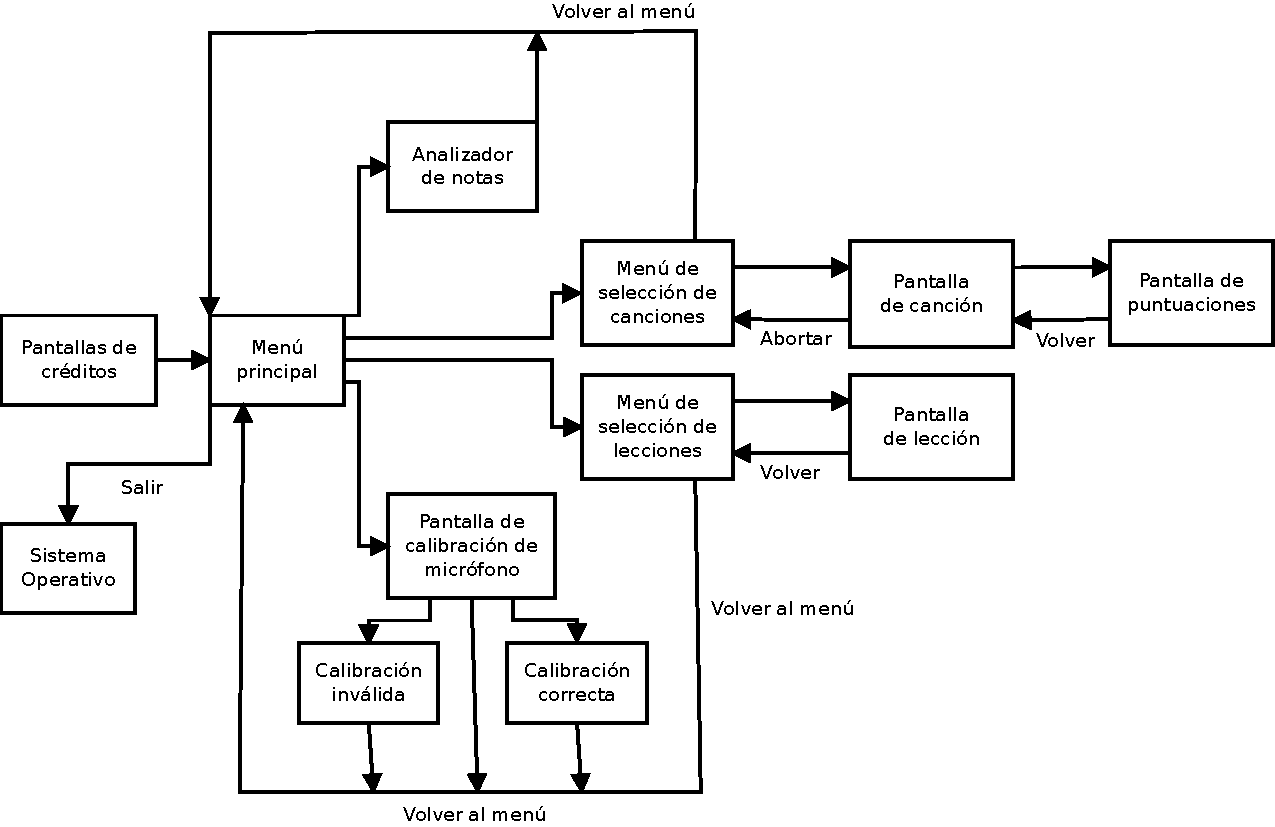
\includegraphics[width=0.9\textwidth]{4_analisis/imagen_diagrama_de_flujo}
  \caption{Diagrama de flujo de las pantallas de oFlute}
\end{figure}

\pagebreak

Inicialmente, deberán aparecer unas pantallas de crédito con información sobre
el desarrollador y sobre el propio videojuego. Tras las mismas, que deberá ser
posible omitir, habrá de aparecer el \textbf{menú principal}, con las cinco
opciones posibles.

\begin{figure}[h!]
  \centering
  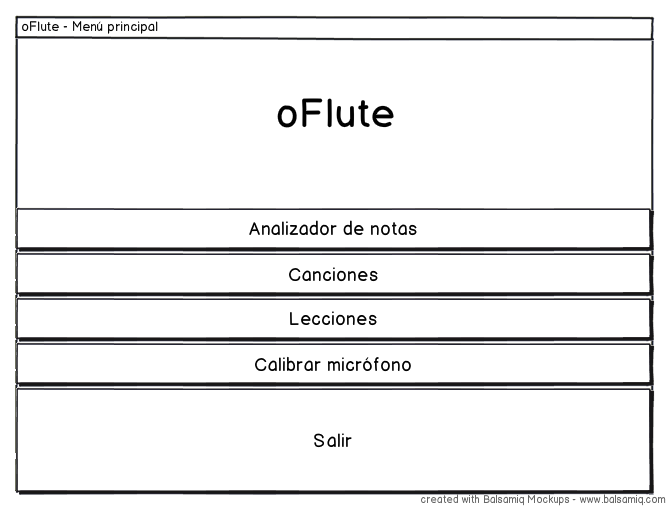
\includegraphics[width=0.6\textwidth]{4_analisis/imagen_mockup_menu_principal}
  \caption{Maqueta del menú principal}
\end{figure}

\pagebreak

Las opciones que se incluirán son:
\begin{itemize}
\item \textbf{Analizador de notas}: comprobar las notas que tocamos sobre un
  pentagrama.
\item \textbf{Canciones}: sección principal del juego, en el que aparecerán las
  canciones a tocar.
\item \textbf{Lecciones}: sección de lecciones de aprendizaje.
\item \textbf{Calibrar micrófono}, para ajustarse al nivel de ruido ambiental.
\item \textbf{Salir} al sistema operativo.
\end{itemize}

La siguiente pantalla a modelar será el \textbf{analizador de
  notas}. Simplemente mostrará el logotipo del videojuego a un lado, y un
pentagrama al otro, que se actualizará con la nota detectada por el
micrófono. También contendrá un botón \textit{volver} para ir al menú principal.

\begin{figure}[h!]
  \centering
  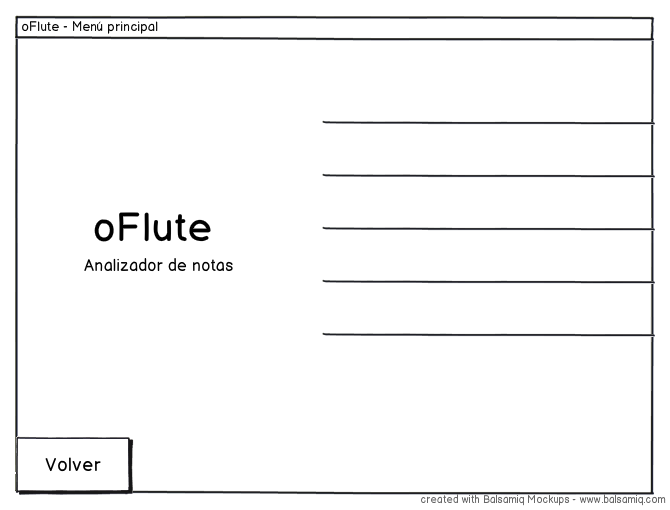
\includegraphics[width=0.6\textwidth]{4_analisis/imagen_mockup_analizador}
  \caption{Maqueta de la sección \textit{analizador de notas}}
\end{figure}

La segunda sección a la que se podrá ir desde el menú principal será la de
\textbf{canciones}. Inicialmente, la primera pantalla será la de
\textbf{selección de canción}, que contendrá el logotipo del juego, un botón
para volver al menú principal, y un menú dinámico de canciones que nos permitirá
elegir el tema a interpretar.

\begin{figure}[h!]
  \centering
  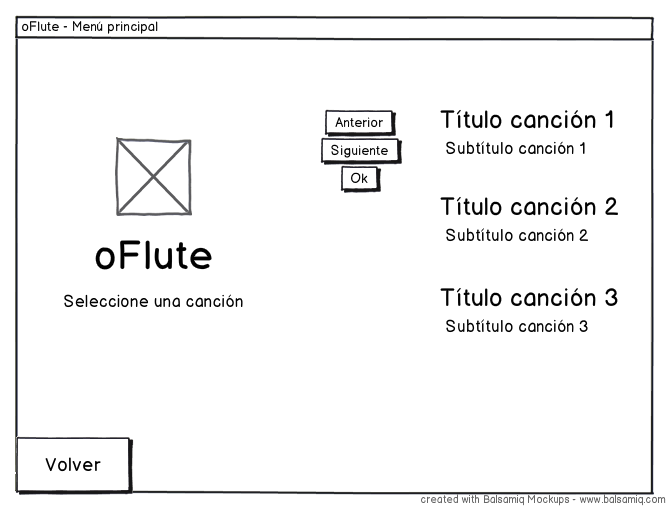
\includegraphics[width=0.6\textwidth]{4_analisis/imagen_mockup_seleccionar_cancion}
  \caption{Maqueta del menú de selección de canción}
\end{figure}

Una vez seleccionada la canción, pasaremos a la zona de \textbf{interpretación
  de canción}. Contendrá un pentagrama que ocupará todo el ancho de la pantalla,
con una línea que indicará la zona donde empezar a tocar las notas que
aparezcan. Además, en la parte superior habrá un indicador con la puntuación
obtenida y, abajo, una barra de progreso que nos indicará cuánto queda de
canción.

\begin{figure}[h!]
  \centering
  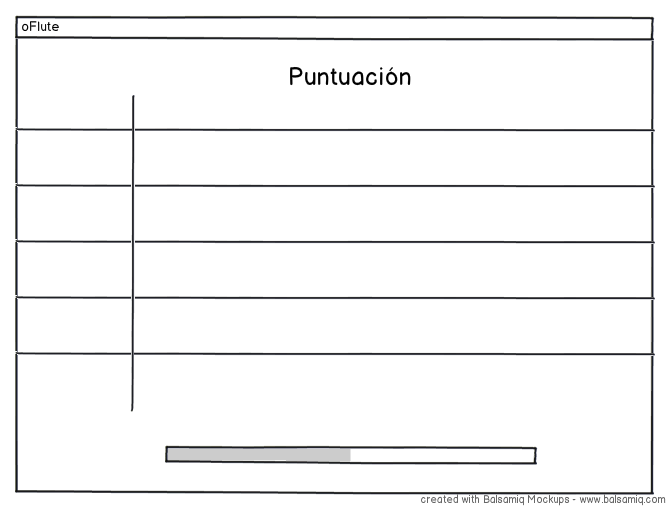
\includegraphics[width=0.6\textwidth]{4_analisis/imagen_mockup_reproducir_cancion}
  \caption{Maqueta de la pantalla de interpretación de canción}
\end{figure}

\pagebreak

Al completar la interpretación de la canción, aparecerá la \textbf{sección de
  resultados}. Contendrá el logotipo del juego, el título y subtítulo de la
canción, y un cuadro con información sobre nuestra interpretación, representada
en forma de porcentaje de aciertos. Además, en la zona inferior aparecerá un
mensaje de ánimo dependiendo del resultado obtenido.

\begin{figure}[h!]
  \centering
  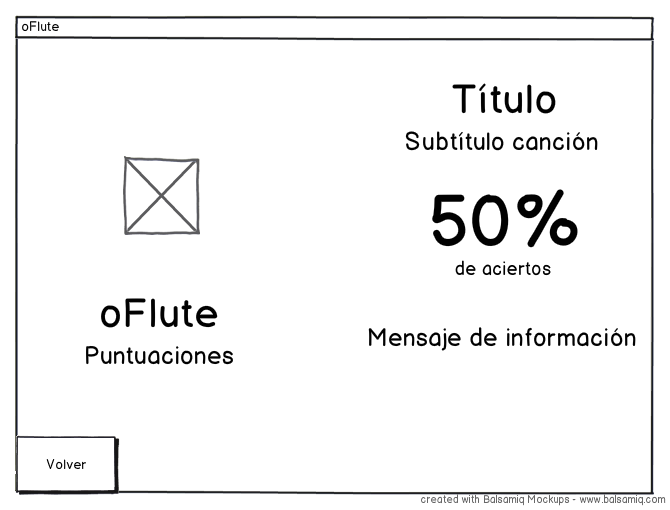
\includegraphics[width=0.6\textwidth]{4_analisis/imagen_mockup_puntuaciones}
  \caption{Maqueta de la pantalla de puntuaciones}
\end{figure}

La pantalla de \textbf{selección de lecciones}, a la que se llega desde el menú
principal, contendrá el título, una imagen decorativa, y varios botones para
navegar entre las lecciones cargadas en el sistema. Se mostrará el título y la
descripción de cada lección, así como un botón para comenzar.

\begin{figure}[h!]
  \centering
  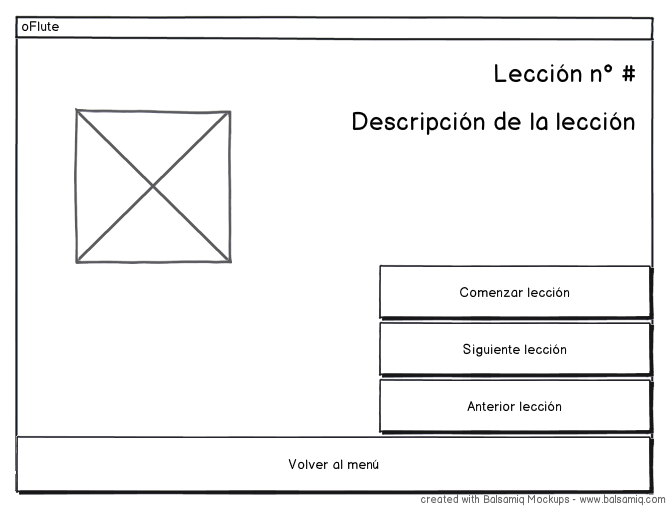
\includegraphics[width=0.6\textwidth]{4_analisis/imagen_mockup_seleccionar_leccion}
  \caption{Maqueta del menú de selección de lecciones}
\end{figure}

Una vez elegida una lección, pasaremos a la pantalla de reproducción de
lecciones. Dada la naturaleza \textbf{dinámica} de esta sección, cada lección
podrá tener una apariencia y elementos distintos. El único elemento común entre
todas las lecciones será el botón de \textbf{volver al menú}.

\subsection{Requisitos funcionales}

\textbf{oFlute} se basa en los siguientes requisitos funcionales:
\begin{itemize}
\item Poder terminar la aplicación pulsando el botón de cierre en cualquier
  instante.
\item Comprobar la correcta interpretación de notas individuales mediante el
  analizador de notas.
\item Calibrar el micrófono de forma que el sistema se pueda adaptar al ruido
  ambiental del entorno.
\item Navegar por toda la aplicación de forma sencilla utilizando solo el ratón.
\item Elegir entre varias canciones a interpretar, cada una con su título y
  subtítulo informativos.
\item Interpretar las canciones mediante el uso de la flauta, siguiendo el
  pentagrama en pantalla.
\item Elegir entre bastantes lecciones informativas, poder ejecutarlas y
  seguirlas.
\item Capacidad de añadir nuevas lecciones y canciones de forma sencilla.
\end{itemize}

\subsection{Requisitos de rendimiento}

La aplicación \textbf{oFlute} precisa de unos requisitos bastante básicos,
que en su mayor parte se reducen a cuatro puntos principales:
\begin{itemize}
\item Posesión de una tarjeta de sonido o subsistema de audio similar con un
  micrófono, para poder captar el sonido de la flauta.
\item Pantalla con una resolución de, al menos, 800 por 600 píxeles.
\item Sistema gráfico compatible con OpenGL.
\item Dispositivo apuntador, como un ratón.
\end{itemize}

La práctica totalidad de los ordenadores personales de la actualidad cumplen los
citados requisitos.

\subsection{Requisitos del sistema software}
El sistema de software deberá cumpliar los requisitos siguientes:
\begin{itemize}
\item Deberá funcionar en cualquier sistema \textbf{GNU/Linux} con los
  requisitos anteriormente indicados.
\item Deberá limitarse el número de dependencias, así como facilitar al máximo
  la instalación de las que resultasen imprescindibles.
\item El uso del teclado quedará en segundo plano, haciendo posible utilizar la
  aplicación completamente con el ratón.
\item Al tratarse de un público objetivo juvenil, la aplicación deberá ser
  dinámica, intuitiva y fácil de usar, y la apariencia debe ser agradable.
\item Se evitará el uso de constantes y recursos dentro del código de la
  aplicación, utilizando como alternativa ficheros para representar las
  lecciones y las canciones.
\end{itemize}

\section{Modelo de casos de uso}

A la hora de modelar los casos de uso del sistema, hemos optado por utilizar
notación \textit{UML}, siguiendo los siguientes pasos:
\begin{itemize}
\item Identificación de los usuarios del sistema y sus roles.
\item Para cada rol, determinar las formas de interactuar con el sistema.
\item Creación de casos de uso para los objetivos que debe cumplir la aplicación.
\item Modularización de los casos de usos mediante la implementación de
  relaciones de inclusión o extensión.
\end{itemize}

\subsection{Diagrama de casos de uso}

\begin{figure}[h!]
  \centering
  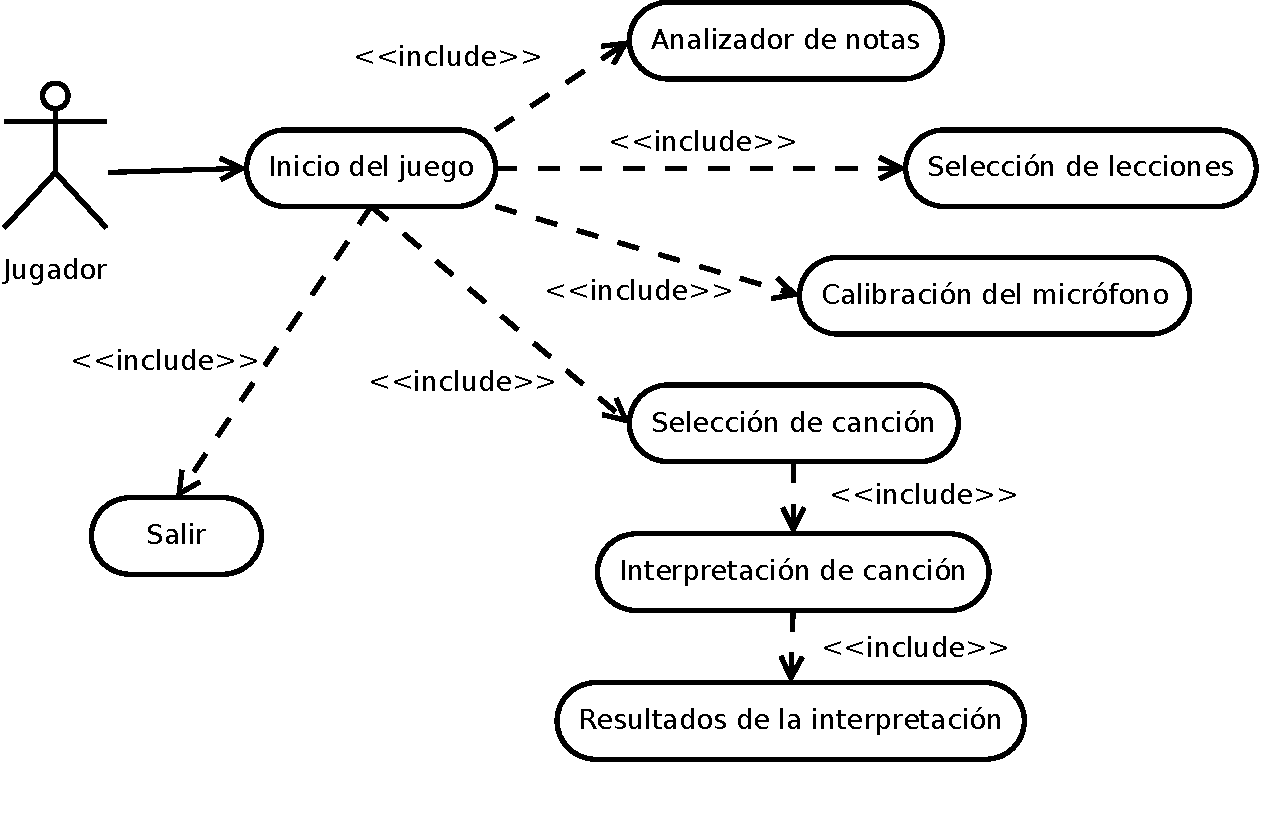
\includegraphics[width=0.81\textwidth]{4_analisis/imagen_diagrama_de_casos_de_uso}
  \caption{Diagrama de casos de uso}
\end{figure}


\subsection{Descripción de los casos de uso}

\subsubsection{Caso de uso: inicio del juego}
\begin{description}
\item [Descripción] Se muestran los créditos del juego, la pantalla de
  presentación, y finalmente el menú principal, desde donde se accederá al
  resto de secciones del juego.
\item [Actores] \jugador.
\item [Precondiciones] Ninguna.
\item [Postcondiciones] Ninguna.
\item [Escenario principal] $\quad$
  \begin{enumerate}
  \item El \jugador\ inicia la aplicación.
  \item El \sistema\ inicializa el subsistema gráfico.
  \item El \sistema\ muestra la pantalla de créditos y la pantalla de
    presentación de la aplicación.
  \item El \sistema\ muestra el menú principal en la pantalla.
  \item El \jugador\ selecciona la opción \textit{Canciones}.
  \item El \sistema\ accede a la pantalla de \textit{Selección de canción}.
  \end{enumerate}
\item[Extensiones --- flujo alternativo] $\quad$
  \begin{description}
  \item [*a] El \jugador\ cierra la ventana.
    \begin{enumerate}
    \item El \sistema\ libera los recursos y sale de la aplicación.
    \end{enumerate}
  \item [4a] El \jugador\ selecciona la opción \textit{Analizador de Notas}.
    \begin{enumerate}
    \item El \sistema\ accede a la pantalla del analizador de notas.
    \end{enumerate}

  \item[4b] El \jugador\ selecciona la opción \textit{Lecciones}.
    \begin{enumerate}
    \item El \sistema\ accede a la pantalla de \textit{Selección de lecciones}.
    \end{enumerate}
  \item[4c] El \jugador\ selecciona la opción \textit{Calibrar micrófono}.
    \begin{enumerate}
    \item El \sistema\ accede a la pantalla de calibración de micrófono.
    \end{enumerate}
  \item [4d] El \jugador\ selecciona la opción Salir.
    \begin{enumerate}
    \item El \sistema\ libera los recursos y sale de la aplicación.\\
    \end{enumerate}
  \end{description}  
\end{description}


\subsubsection{Caso de uso: selección de canción}

\begin{description}
\item [Descripción] Al \jugador\ se le muestra una lista de las canciones
  detectadas, y éste debe elegir entre ellas la que desea interpretar, o volver
  al menú princial.
\item [Actores] \jugador.
\item [Precondiciones] Ninguna.
\item [Postcondiciones] Una canción queda seleccionada.
\item [Escenario principal] $\quad$
  \begin{enumerate}
  \item El \jugador\ accede, desde el menú principal, al panel de selección de canciones.
  \item El \sistema\ busca las canciones dadas de alta en el juego y muestra un menú con las mismas.
  \item El \jugador\ navega entre las canciones listadas y selecciona una de ellas, pulsando finalmente el botón \textit{Ok}.
  \item El \sistema\ carga la canción y pasa a la pantalla de interpretación de canciones.
  \end{enumerate}
\item[Extensiones --- flujo alternativo] $\quad$
  \begin{description}
  \item [*a] El \jugador\ cierra la ventana.
    \begin{enumerate}
    \item El \sistema\ libera los recursos y sale de la aplicación.
    \end{enumerate}
  \item [3a] El \jugador\ selecciona la opción \textit{Volver}.
    \begin{enumerate}
    \item El \sistema\ muestra la animación de cierre y vuelve al menú principal.
    \end{enumerate}
  \end{description}  
\end{description}


\subsubsection{Caso de uso: interpretación de canción}

\begin{description}
\item [Descripción] Tras haber elegido la canción a interpretar, se muestra una
  partitura con las notas que el \jugador\ deberá tocar para conseguir la puntuación deseada.
\item [Actores] \jugador.
\item [Precondiciones] Se ha elegido una canción.
\item [Postcondiciones] Se completa la interpretación de la canción, obteniendo una calificación
\item [Escenario principal] $\quad$
  \begin{enumerate}
  \item El \sistema\ carga la canción, leyendo las notas, y muestra en pantalla,
    mediante animaciones, el marcador de puntos y el pentagrama.
  \item El \sistema\ comienza a mostrar notas en el pentagrama, que van
    deslizándose hacia el lado izquierdo, en el que se encuentra la aguja de
    reproducción, e inicia el análisis del sonido.
  \item El \jugador\, al llegar la nota a la aguja de reproducción, toca la
    flauta con la altura y la duración correcta, de forma que el micrófono sea
    capaz de captar el sonido.
  \item El \sistema\ analiza el sonido que captura el micrófono y detecta la nota que toca el usuario.
  \item El \sistema\ determina que la nota es la correcta y suma los puntos correspondientes.
  \item Mientras existan más notas, se vuelve al punto 2.
  \item El \sistema\ determina que no hay más notas que mostrar, e inicia las
    animaciones para ocultar los elementos en pantalla.
  \item El \sistema\ pasa a la sección de \textit{Resultados de la interpretación}.
  \end{enumerate}
\item[Extensiones --- flujo alternativo] $\quad$
  \begin{description}

  \item [*a] El \jugador\ cierra la ventana.
    \begin{enumerate}
    \item El \sistema\ libera los recursos y sale de la aplicación.
    \end{enumerate}

  \item[*b] El \jugador\ pulsa la tecla \texttt{escape}.
    \begin{enumerate}
    \item El \sistema\ vuelve a la pantalla de \textit{selección de canción}.
    \end{enumerate}

  \item [3a] El \jugador\ toca el instrumento con intensidad insuficiente o nula
    y el sonido no llega al sistema.
    \begin{enumerate}
    \item El \sistema\ representa esta inconsistencia como un silencio.
    \end{enumerate}

  \item [4a] El \sistema\ no es capaz de determinar fehacientemente la nota que
    toca el usuario.
    \begin{enumerate}
    \item El \sistema\ representa esta inconsistencia como un silencio.
    \end{enumerate}

  \item[5a] El \sistema\ determina que la nota tocada por el usuario no es la
    que corresponde a la partitura.
    \begin{enumerate}
    \item El \sistema\ ignora esta situación y no suma los puntos al marcador.
    \end{enumerate}

  \end{description}  
\end{description}

\subsubsection{Caso de uso: resultados de la interpretación}

\begin{description}
\item [Descripción] Después de interpretar las notas de la partitura, se
  muestran los datos obtenidos del análisis de las notas tocadas por el \jugador.
\item [Actores] \jugador.
\item [Precondiciones] Se ha elegido e interpretado una canción.
\item [Postcondiciones] Se completa la partida actual.
\item [Escenario principal] $\quad$
  \begin{enumerate}
  \item El \sistema\ compara la puntuación conseguida con la máxima puntuación
    obtenible, y genera un porcentaje de aciertos.
  \item El \sistema\ muestra, mediante animaciones, un mensaje con información
    sobre la canción y sobre la interpretación del \jugador\, representada
    mediante un porcentaje de aciertos.
  \item El \sistema\ muestra un mensaje variable en función del número de
    aciertos conseguido.
  \item El \jugador\ revisa su puntuación y pulsa el botón \textit{volver} para
    ir de vuelta al menú de \textit{selección de canción}.
  \end{enumerate}
\item[Extensiones --- flujo alternativo] $\quad$
  \begin{description}

  \item [*a] El \jugador\ cierra la ventana.
    \begin{enumerate}
    \item El \sistema\ libera los recursos y sale de la aplicación.
    \end{enumerate}

  \item[4a] El \jugador\ pulsa la tecla \texttt{escape}.
    \begin{enumerate}
    \item El \sistema\ vuelve a la pantalla de \textit{selección de canción}.
    \end{enumerate}

  \end{description}  
\end{description}


\subsubsection{Caso de uso: analizador de notas}

\begin{description}
\item [Descripción] El \jugador\ elige la opción \textit{analizador de notas} en
  el menú principal y es llevado a esta sección, en la que el sistema
  representará gráficamente la nota que esté tocando con la flauta en cada
  instante, sin otra interacción
\item [Actores] \jugador.
\item [Precondiciones] Ninguna.
\item [Postcondiciones] Ninguna
\item [Escenario principal] $\quad$
  \begin{enumerate}
  \item El \jugador\ accede, desde el menú principal, al panel del analizador de notas.
  \item El \sistema\ muestra, mediante animaciones, la pantalla de la sección,
    representada mediante una fracción de partitura en la que se representará la
    nota que esté tocando el \jugador\ en cada momento.
  \item El \sistema\ inicia el análisis del sonido.
  \item El \jugador\ toca la nota que desee con su flauta, de forma que el
    micrófono sea capaz de captar el sonido.
  \item El \sistema\ analiza el sonido que captura el micrófono y detecta la
    nota que toca el usuario.
  \item El \sistema\ muestra en pantalla la nota, sobre la partitura,
    correspondiente a lo que ha tocado el usuario.
  \item Se repite el flujo desde el punto 4, mientras el \jugador\ no pulse en
    el botón volver.
  \item El \jugador\ pulsa en el botón \textit{volver}.
  \item El \sistema\ inicia las animaciones para ocultar los elementos en pantalla.
  \item El \sistema\ vuelve al menú principal.
  \end{enumerate}
\item[Extensiones --- flujo alternativo] $\quad$
  \begin{description}

  \item [*a] El \jugador\ cierra la ventana.
    \begin{enumerate}
    \item El \sistema\ libera los recursos y sale de la aplicación.
    \end{enumerate}

  \item[*b] El \jugador\ pulsa la tecla \texttt{escape}.
    \begin{enumerate}
    \item El \sistema\ vuelve al menú principal.
    \end{enumerate}

  \item [4a] El \jugador\ toca el instrumento con intensidad insuficiente o nula
    y el sonido no llega al sistema.
    \begin{enumerate}
    \item El \sistema\ representa esta inconsistencia como un silencio.
    \end{enumerate}

  \item [5a] El \sistema\ no es capaz de determinar fehacientemente la nota que
    toca el usuario.
    \begin{enumerate}
    \item El \sistema\ representa esta inconsistencia como un silencio.
    \end{enumerate}
  \end{description}  
\end{description}

\subsubsection{Caso de uso: calibración de micrófono}
\begin{description}
\item [Descripción] El \jugador\ elige la opción \textit{calibrar micrófono} en
  el menú principal y es llevado a esta sección, en la que el \sistema\ calibrará
  el micrófono de forma que sea posible aislar el sonido de la flauta del ruido
  ambiental.
\item [Actores] \jugador.
\item [Precondiciones] Ninguna.
\item [Postcondiciones] El \sistema\ obtiene un valor umbral con el que
  discernir entre el sonido del instrumento y el ruido ambiente.
\item [Escenario principal] $\quad$
  \begin{enumerate}
  \item El \jugador\ accede, desde el menú principal, al panel de calibración del micrófono.
  \item El \sistema\ muestra la sección, indicando con un mensaje que el usuario
    debe pulsar la tecla \texttt{escape} para iniciar la calibración.
  \item El \jugador\ pulsa la tecla \texttt{escape} y se mantiene en silencio.
  \item El \sistema\ inicia el análisis del sonido, guardando durante dos
    segundos los valores de ruido que lee del micrófono.
  \item El \sistema\ calcula, a partir de los valores leídos, el umbral de
    ruido, y muestra un mensaje informando del final del proceso.
  \item El \jugador\ pulsa la tecla \texttt{escape} y el \sistema\ vuelve al
    menú principal.
  \end{enumerate}
\item[Extensiones --- flujo alternativo] $\quad$
  \begin{description}

  \item [*a] El \jugador\ cierra la ventana.
    \begin{enumerate}
    \item El \sistema\ libera los recursos y sale de la aplicación.
    \end{enumerate}

  \item[*b] El \jugador\ pulsa la tecla \texttt{escape}.
    \begin{enumerate}
    \item El \sistema\ cancela la calibración y vuelve al menú principal.
    \end{enumerate}

  \item [5a] El \sistema\ encuentra valores inválidos al leer el ruido
    ambiental.
    \begin{enumerate}
    \item El \sistema\ informa al usuario del fallo del proceso de calibración.
    \item El \jugador\ pulsa la tecla \texttt{escape} y el \sistema\ vuelve al
      menú principal.
    \end{enumerate}
  \end{description}  
\end{description}

\subsubsection{Caso de uso: selección de lecciones}
\begin{description}
\item [Descripción] El \jugador\ elige la opción \textit{lecciones} en el menú
  principal y es llevado a esta sección, en la que el \sistema\ mostrará una
  lista de lecciones cargadas, entre las que el usuario deberá elegir.
\item [Actores] \jugador.
\item [Precondiciones] Ninguna.
\item [Postcondiciones] Se ha elegido una lección
\item [Escenario principal] $\quad$
  \begin{enumerate}
  \item El \jugador\ accede, desde el menú principal, al panel de selección de lecciones.
  \item El \sistema\ carga la lista de secciones y muestra, mediante
    animaciones, el panel, preseleccionando por defecto la primera lección.
  \item El \jugador\ utiliza los botones de la sección para elegir una de las
    lecciones, y activarla pulsando \textit{comenzar lección}.
  \item El \sistema\ oculta de forma animada el panel de selección de lecciones.
  \item El \sistema\ lee el fichero \texttt{xml} asociado a la lección indicada,
    cargando los elementos que la componen y las animaciones que se ejecutarán.
  \item El \sistema\ ejecuta las animaciones correspondientes a los elementos
    multimedia de la lección.
  \end{enumerate}
\item[Extensiones --- flujo alternativo] $\quad$
  \begin{description}

  \item [*a] El \jugador\ cierra la ventana.
    \begin{enumerate}
    \item El \sistema\ libera los recursos y sale de la aplicación.
    \end{enumerate}

  \item[2a] El \sistema\ detecta que una de las lecciones leídas no está
    correctamente construída.
    \begin{enumerate}
    \item El \sistema\ informa del error en el \textit{log} del programa y omite
      la carga de esa lección.
    \end{enumerate}

  \item[3a] El \jugador\ pulsa la tecla \texttt{escape}.
    \begin{enumerate}
    \item El \sistema\ vuelve al menú principal.
    \end{enumerate}

  \item[6a] El \jugador\ pulsa la tecla \texttt{escape}.
    \begin{enumerate}
    \item El \sistema\ vuelve al menú de selección de lecciones.
    \end{enumerate}

  \end{description}  
\end{description}

\section{Modelo conceptual de datos}

El modelo conceptual de datos representa, de forma esquemática, las clases que
modelan el sistema y las relaciones que existen entre ellas, además de una
pequeña introducción a su utilidad. 

\begin{description}
\item[Juego] Clase de control general. Gestiona el flujo de ejecución principal,
  así como de la gestión de estados, que permite pasar de una sección a otra del
  juego.
\item[Estado] Clase base para los diferentes estados del juego. Las clases
  correspondientes a las secciones se basarán en esta clase para interactuar con
  el gestor de estados y poder pasar de una parte del juego a otra.
\item[EstadoMenú] Representa el estado de juego para el menú principal, desde el
  que se accede al resto de opciones del juego. 
\item[EstadoAnalizador] Representa el estado del analizador básico de
  notas. Contendrá los elementos necesarios para iniciar el análisis del audio,
  así como los elementos de la interfaz.
\item[EstadoCalibrarMicro] Representa el estado en el que se calibra el
  micrófono. Al igual que la clase \textit{EstadoAnalizador}, deberá ser capaz
  de acceder al sistema de audio para poder leer el volumen ambiente y así
  calibrar el micrófono.
\item[EstadoImagenFija] Modela una imagen fija a modo de pantalla de créditos,
  de forma que sea sencillo añadir imágenes al inicio del juego, como firmas de
  desarrolladores, logotipos de patrocinadores, etcétera.
\item[EstadoMenúCanciones] Comprende el menú de selección de canciones, que se
  encargará de leer los ficheros de canciones disponibles. Además, también se
  encargará de lanzar las canciones en forma de estados secundarios.
\item[EstadoCanción] Corresponde a la canción que se va a interpretar, lanzada desde
  el estado \textit{EstadoMenuCanciones}.
\item[EstadoMenúLecciones] Corresponde al menú de elección de lecciones, que
  leerá y listará los ficheros de lección disponibles, y se encargará de lanzar
  la lección elegida.
\item[EstadoLección] Corresponde a la canción elegida desde el menú
  \textit{EstadoMenúLecciones}.
\item[Analizador] Controla la gestión del subsistema de audio y el análisis de
  la entrada. Deberá proporcionar información sobre el volumen de la entrada
  (para la calibración del micrófono) así como de la nota detectada en cada
  instante.
\item[Animación] Se encargará de facilitar la creación de animaciones en forma
  de interpolación de valores, válidas para cambios de posición, opacidad,
  etcétera.
\item[Elemento] Esta clase de ayuda facilitará la carga y dibujado de elementos
  para la interfaz, además de servir de capa de abstracción para las
  animaciones.
\item[ElementoImagen] Especialización de la clase \textit{Elemento} para
  imágenes.
\item[ElementoTexto] Especialización de la clase \textit{Elemento} para textos.
\item[ElementoCombinado] Especialización de la clase \textit{Elemento} que
  combina imagen y texto, a usar en casos como los botones del menú.
\item[SistemaPartículas] Representa un sistema de partículas simple, para
  generar efectos de destellos y fuegos artificiales.
\item[Nota] Simboliza cada una de las notas cargadas que componen una canción.
\end{description}

\begin{figure}[htp!]
  \centering
  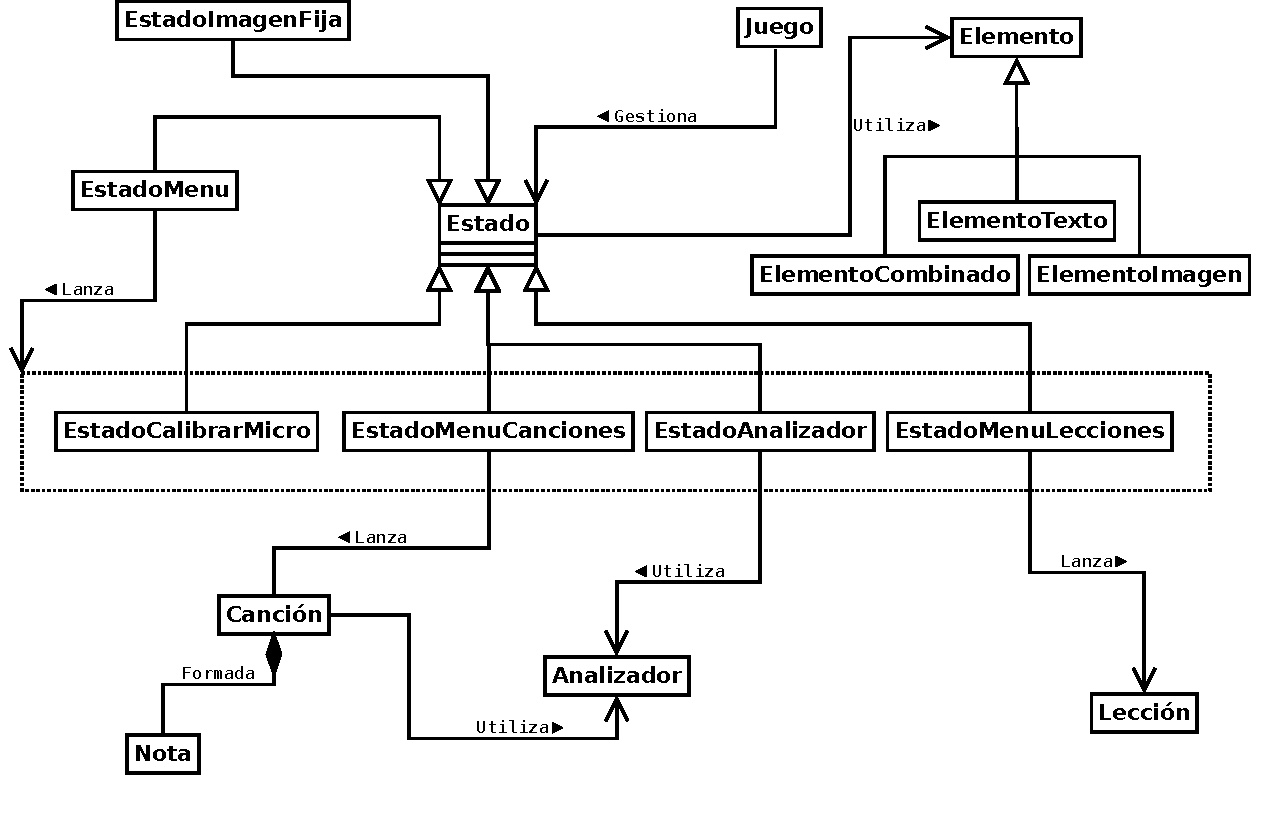
\includegraphics[angle=90]{4_analisis/imagen_diagrama_clases_conceptuales}
  \caption{Diagrama de clases conceptuales}
\end{figure}

\pagebreak


\section{Modelo de comportamiento del sistema}
En esta sección vamos a especificar cómo se comporta el sistema en forma de dos
elementos fundamentales.
\begin{itemize}
\item En primer lugar, los \textbf{diagramas de secuencia} mostrarán el flujo de
  eventos entre los actores que participan en la aplicación.
\item En segundo lugar, los \textbf{contratos de las operaciones} detallarán las
  condiciones y efectos que tendrán lugar al ejecutarse las operaciones en el
  sistema.
\end{itemize}

\begin{nota}
  No se han reflejado, por triviales, los escenarios alternativos en los que el
  usuario cierra la ventana, correspondientes a los flujos \textit{*a} definidos
  en la sección anterior.
\end{nota}

\begin{description}
\item[Operación] 
\item[Actores]
\item[Responsabilidades]
\item[Precondiciones]
\item[Postcondiciones]
\end{description}

\subsection{Caso de uso: inicio del juego}

\subsubsection{Escenario principal}

\begin{figure}[h!]
  \centering
  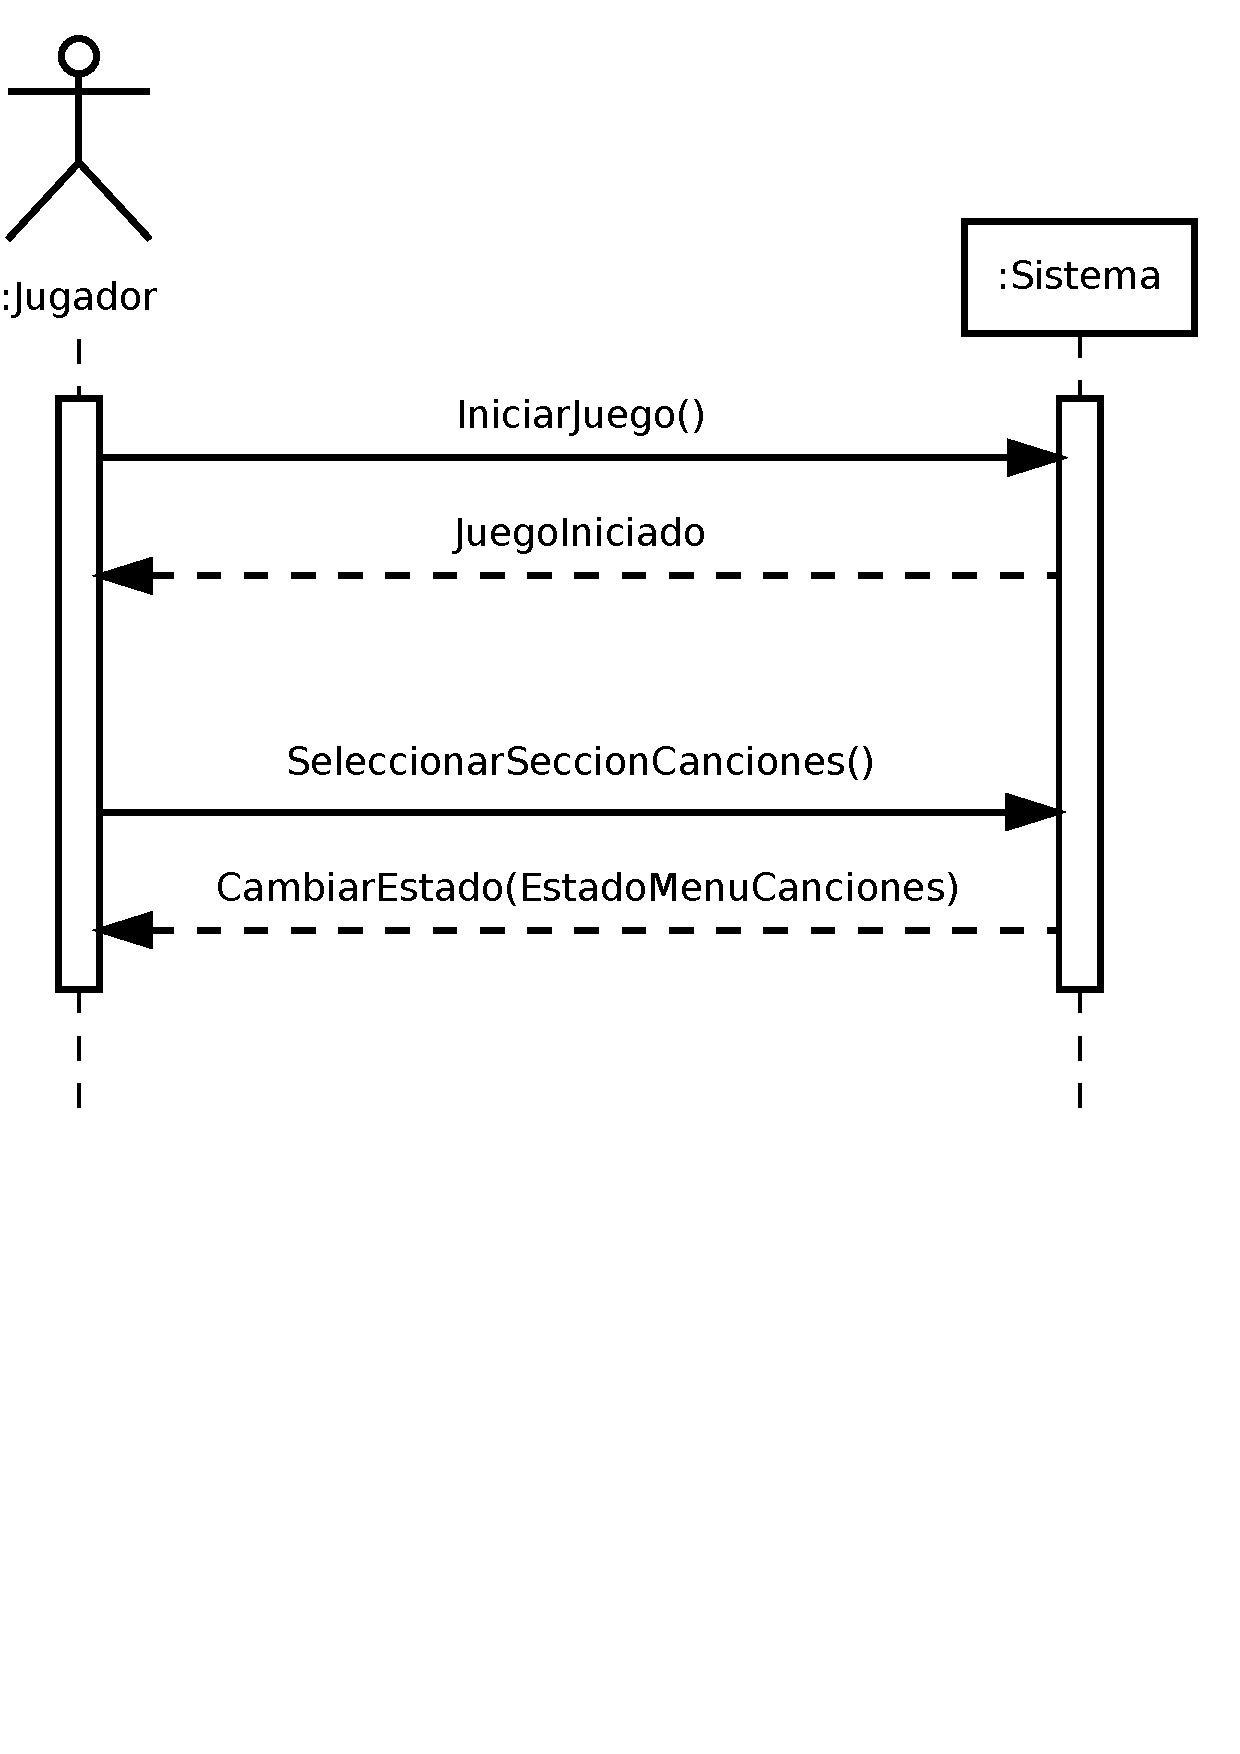
\includegraphics[trim=0cm 12cm 0cm 0cm, clip=true, width=0.5\textwidth]{4_analisis/diagsec_caso1_esc1}
  \caption{Diagrama de secuencia, incio del juego, escenario principal}
\end{figure}

\begin{description}
\item[Operación] IniciarJuego()
\item[Actores] \jugador\, \sistema\
\item[Responsabilidades] Cargar y lanzar la aplicación, mostrar los títulos de
  crédito y el menú principal.
\item[Precondiciones] Ninguna.
\item[Postcondiciones] $\quad$

  \begin{itemize}
  \item Se crea una instancia de la clase \textit{Juego}, que gestiona la
    creación y destrucción de los estados.
  \item Se crean y posteriormente destruyen dos estados
    \textit{EstadoImagenFija} para mostrar los títulos de crédito.
  \item Se crea y permanece un estado \textit{EstadoMenú}, que representa el
    menú principal de la aplicación.
  \end{itemize}

\end{description}

\begin{description}
\item[Operación] SeleccionarSeccionCanciones()
\item[Actores] \jugador\, \sistema\
\item[Responsabilidades] Esconder el menú principal y cargar el menú de
  selección de canciones.
\item[Precondiciones] $\quad$

  \begin{itemize}
  \item El estado actual es una instancia de \textit{EstadoMenú}.
  \end{itemize}

\item[Postcondiciones] Se destruye el estado \textit{EstadoMenú} y se carga
  \textit{EstadoMenúCanciones}.
\end{description}

\subsubsection{Escenario alternativo 4a}
\begin{figure}[h!]
  \centering
  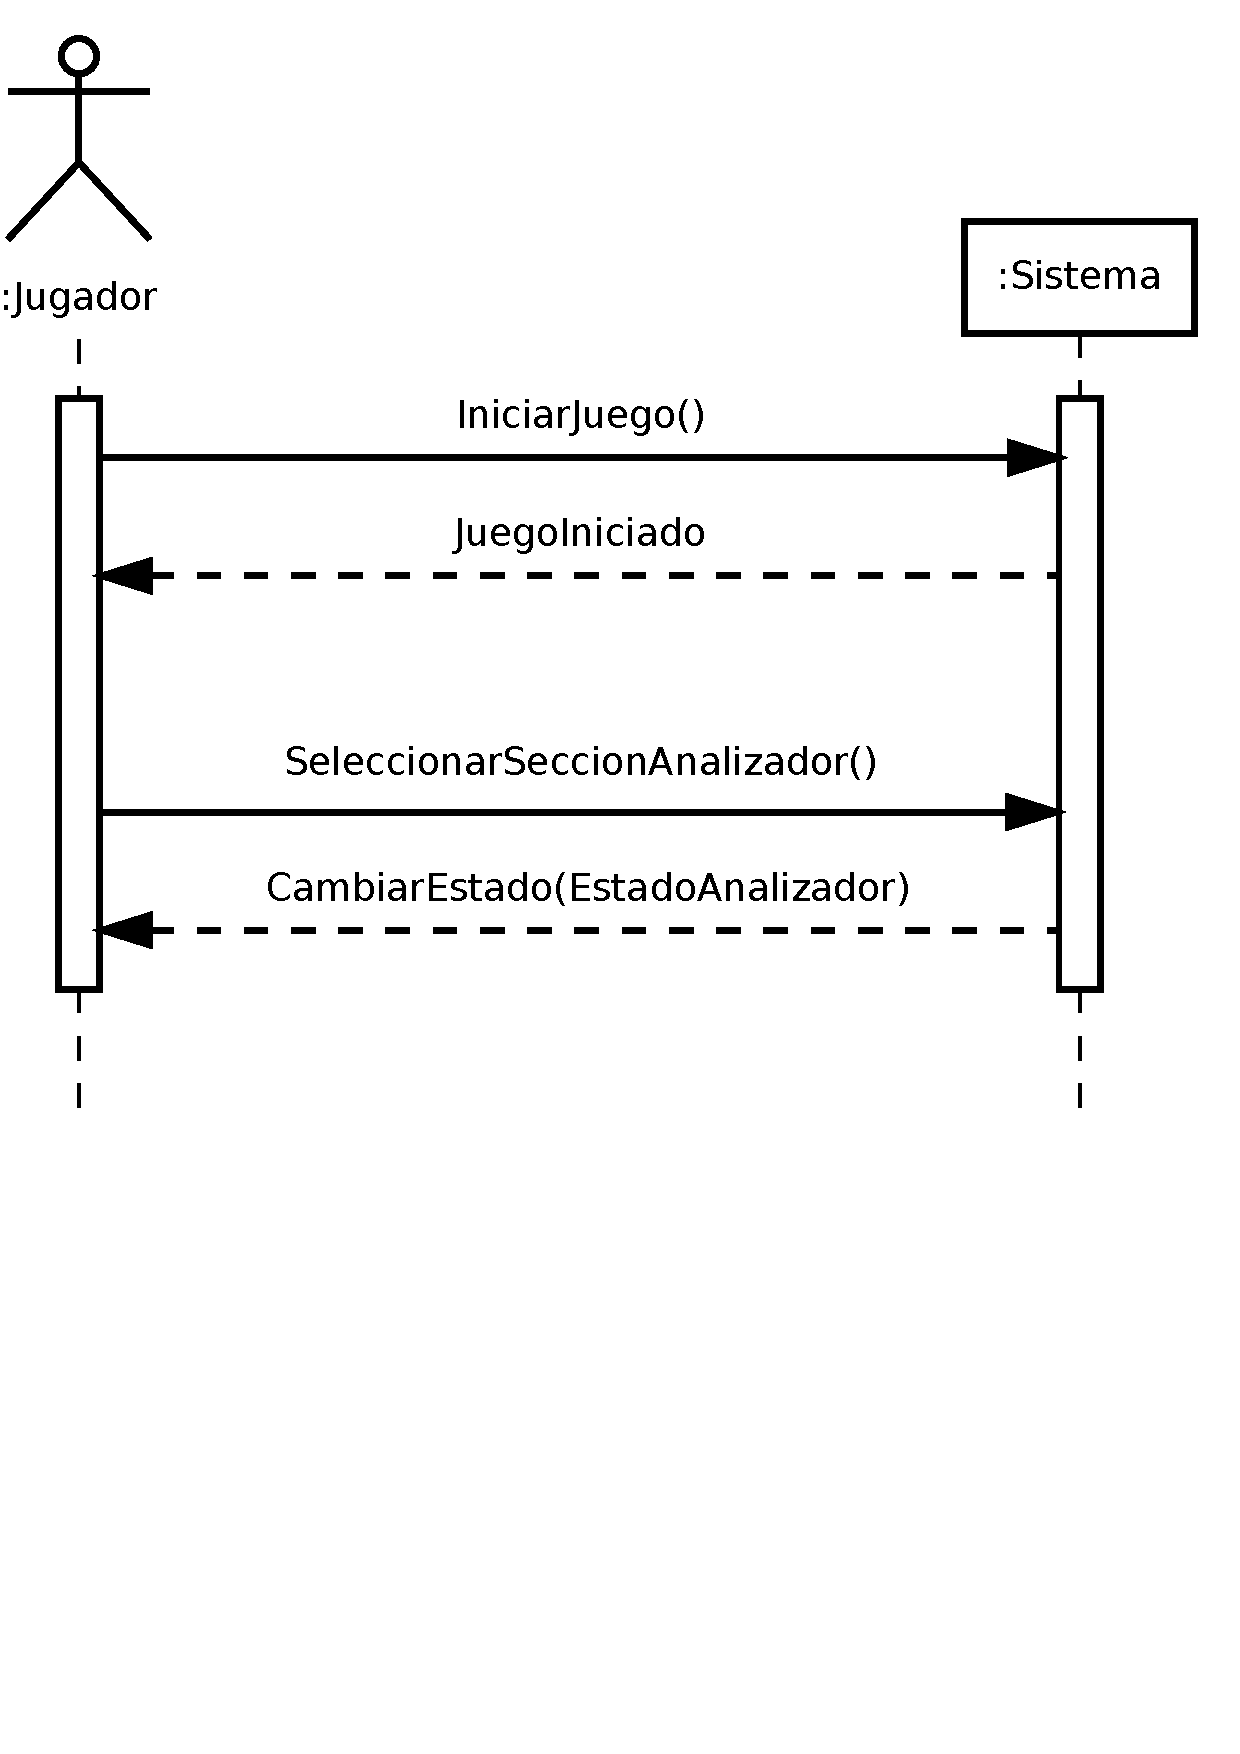
\includegraphics[trim=0cm 12cm 0cm 0cm, clip=true, width=0.5\textwidth]{4_analisis/diagsec_caso1_esc2}
  \caption{Diagrama de secuencia, incio del juego, escenario alternativo 4a}
\end{figure}

\begin{description}
\item[Operación] SeleccionarSeccionAnalizador()
\item[Actores] \jugador\, \sistema\
\item[Responsabilidades] Esconder el menú principal y cargar la sección de
  análisis de notas.
\item[Precondiciones] $\quad$
  \begin{itemize}
  \item El estado actual es una instancia de \textit{EstadoMenú}.
  \end{itemize}
\item[Postcondiciones] Se destruye el estado \textit{EstadoMenú} y se carga
  \textit{EstadoAnalizador}.
\end{description}

\subsubsection{Escenario alternativo 4b}
\begin{figure}[h!]
  \centering
  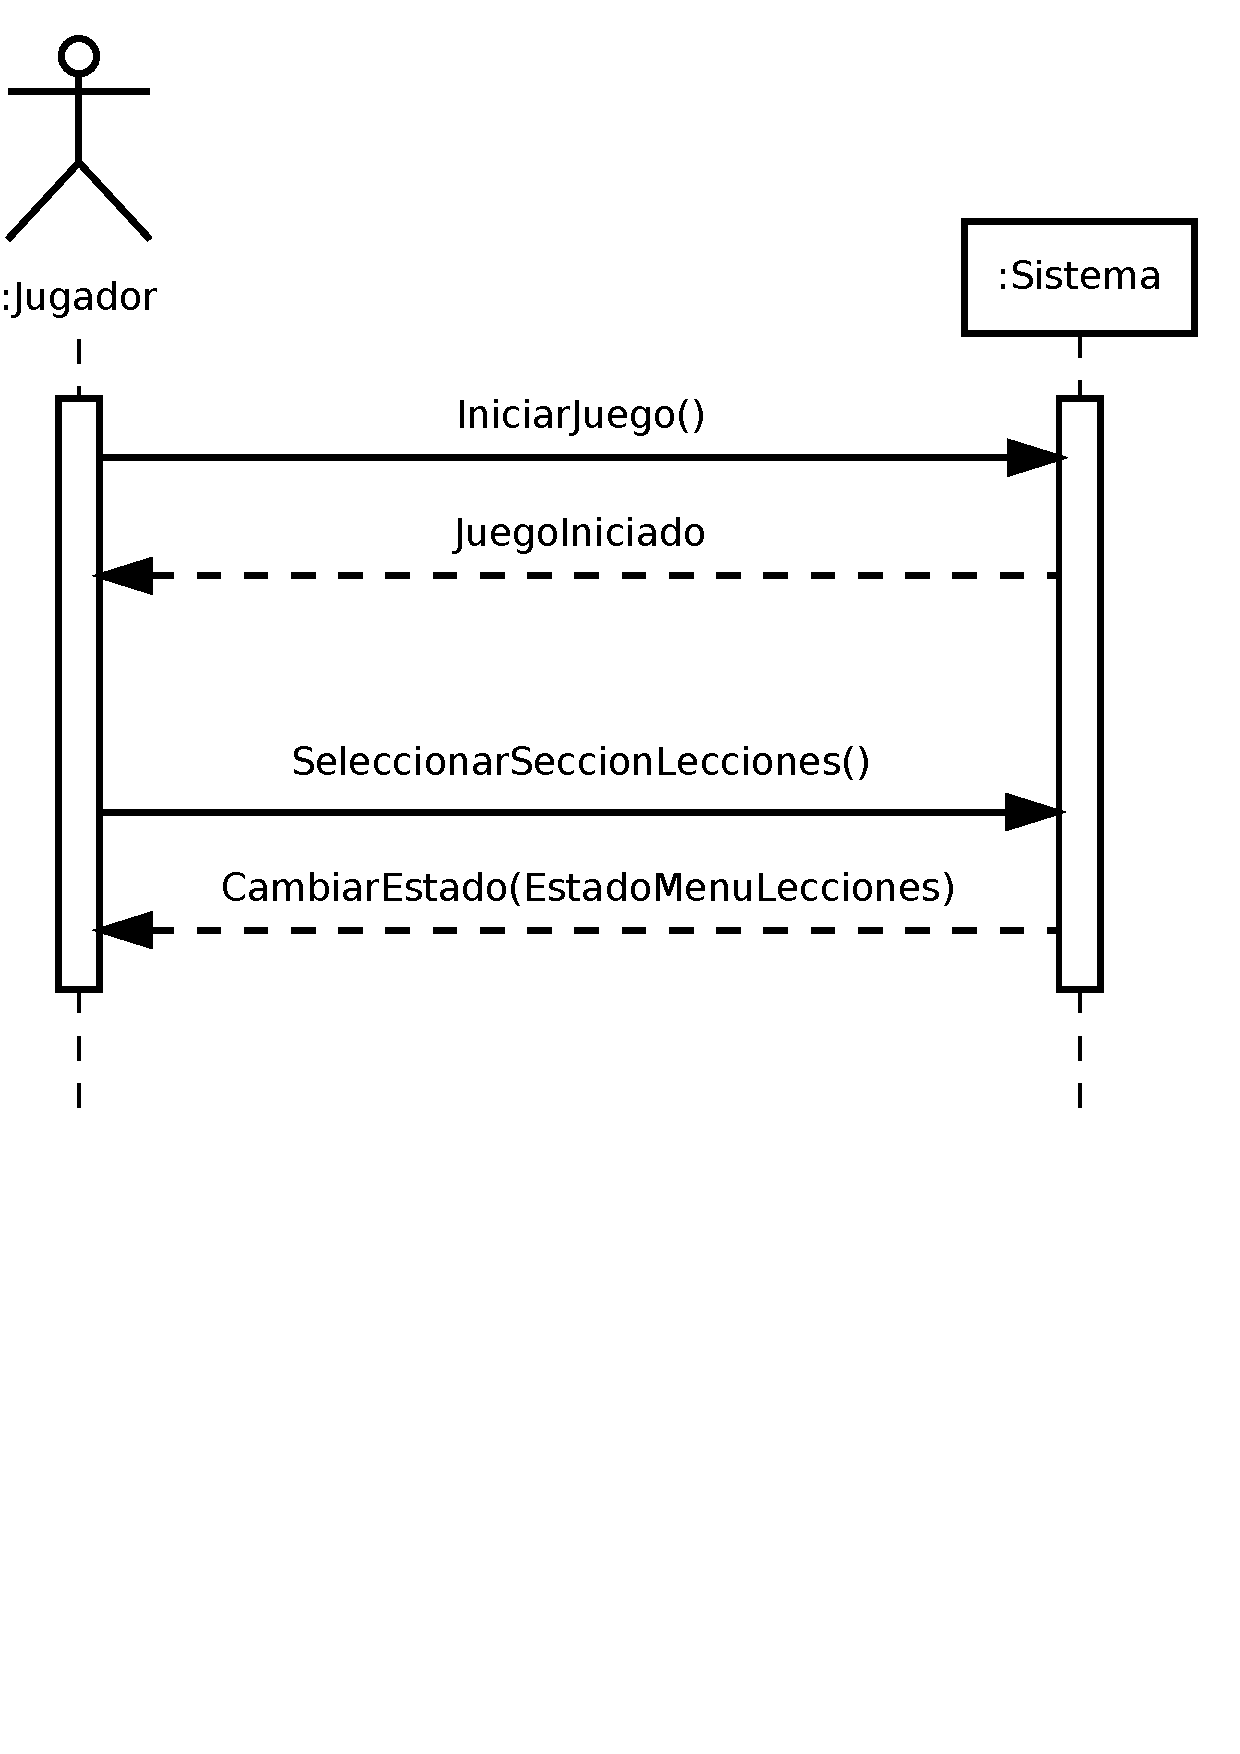
\includegraphics[trim=0cm 12cm 0cm 0cm, clip=true, width=0.5\textwidth]{4_analisis/diagsec_caso1_esc3}
  \caption{Diagrama de secuencia, incio del juego, escenario alternativo 4b}
\end{figure}

\begin{description}
\item[Operación] SeleccionarSeccionLecciones()
\item[Actores] \jugador\, \sistema\
\item[Responsabilidades] Esconder el menú principal y cargar la menú de
  selección de lecciones.
\item[Precondiciones] $\quad$
  \begin{itemize}
  \item El estado actual es una instancia de \textit{EstadoMenú}.
  \end{itemize}
\item[Postcondiciones] Se destruye el estado \textit{EstadoMenú} y se carga
  \textit{EstadoMenúLecciones}.
\end{description}

\subsubsection{Escenario alternativo 4c}
\begin{figure}[h!]
  \centering
  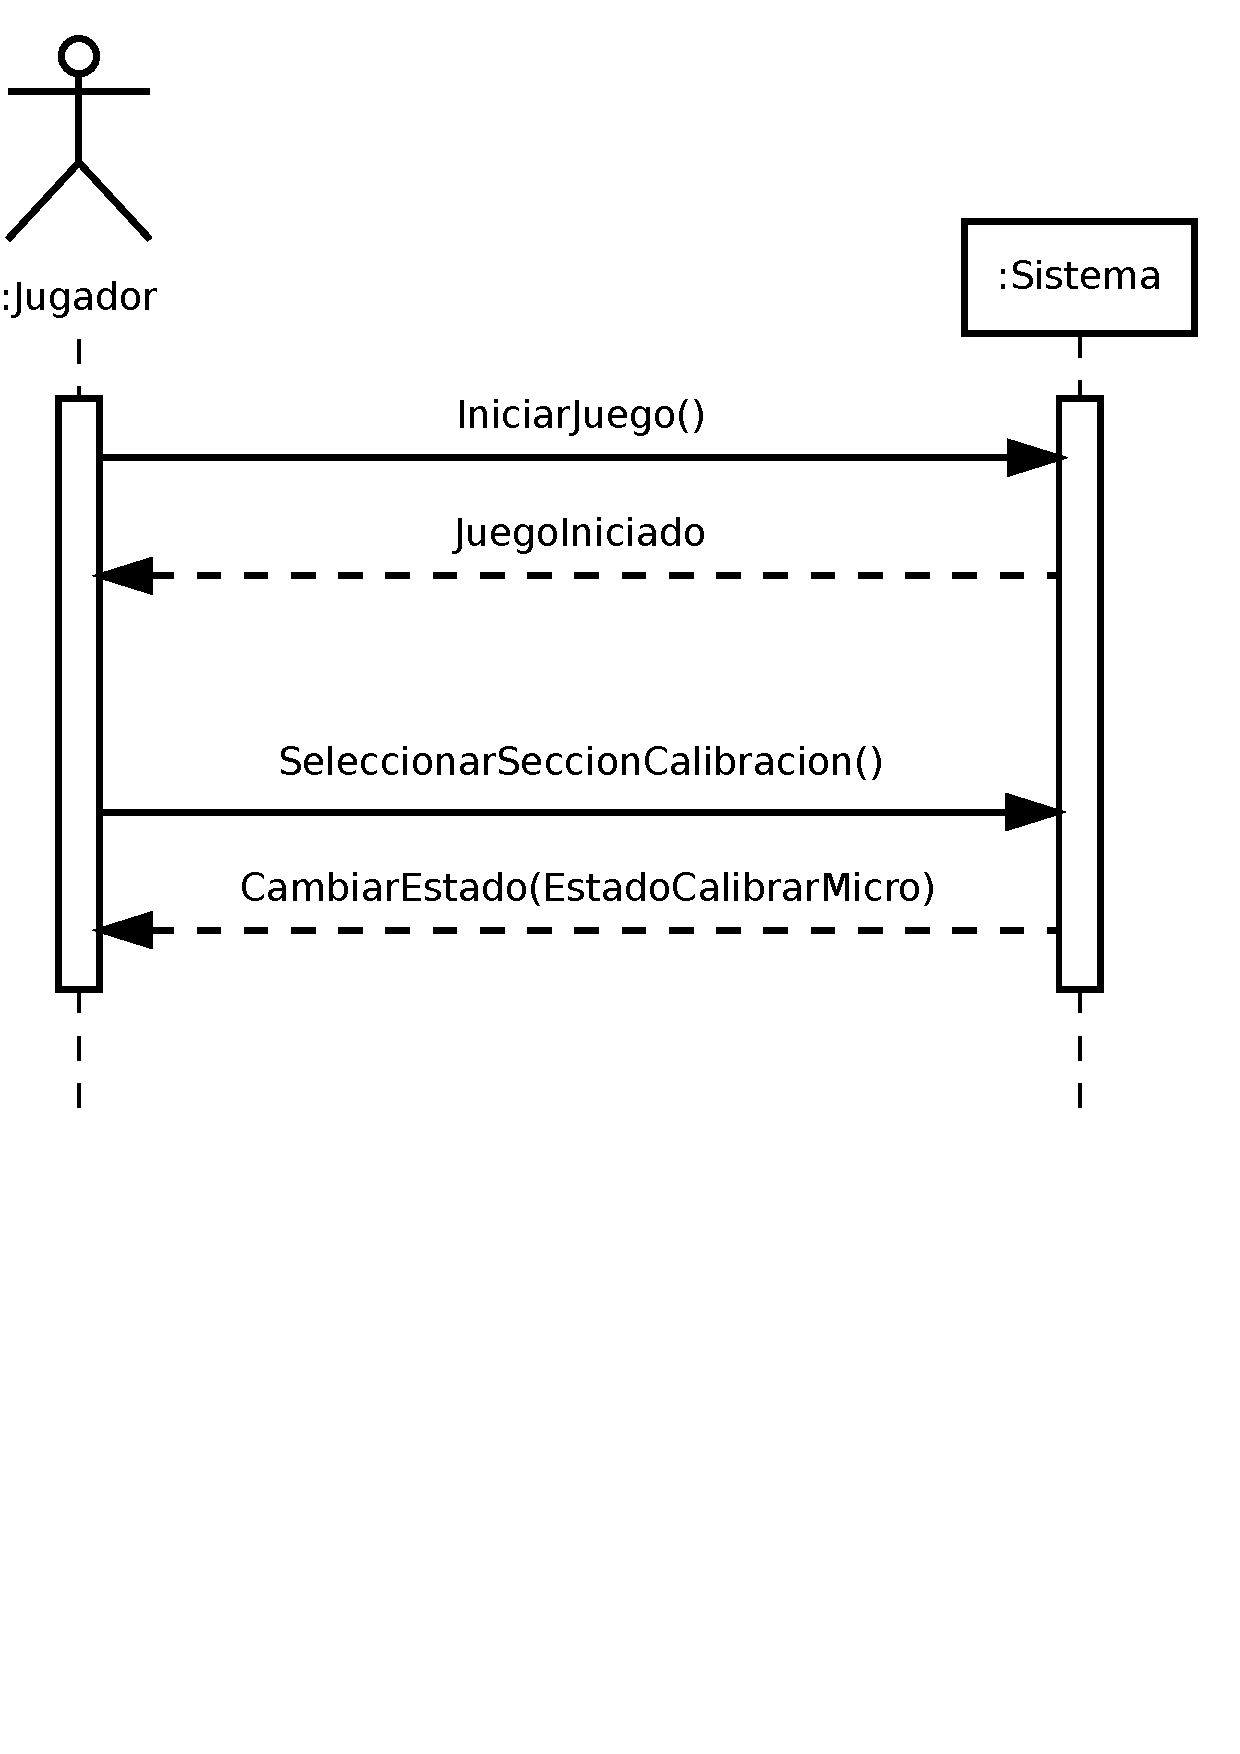
\includegraphics[trim=0cm 12cm 0cm 0cm, clip=true, width=0.5\textwidth]{4_analisis/diagsec_caso1_esc4}
  \caption{Diagrama de secuencia, incio del juego, escenario alternativo 4c}
\end{figure}

\begin{description}
\item[Operación] SeleccionarSeccionCalibracion()
\item[Actores] \jugador\, \sistema\
\item[Responsabilidades] Esconder el menú principal y cargar la sección de
  calibración de micrófono.
\item[Precondiciones] $\quad$
  \begin{itemize}
  \item El estado actual es una instancia de \textit{EstadoMenú}.
  \end{itemize}
\item[Postcondiciones] Se destruye el estado \textit{EstadoMenú} y se carga
  \textit{EstadoCalibrarMicro}.
\end{description}

\subsubsection{Escenario alternativo 4d}
\begin{figure}[h!]
  \centering
  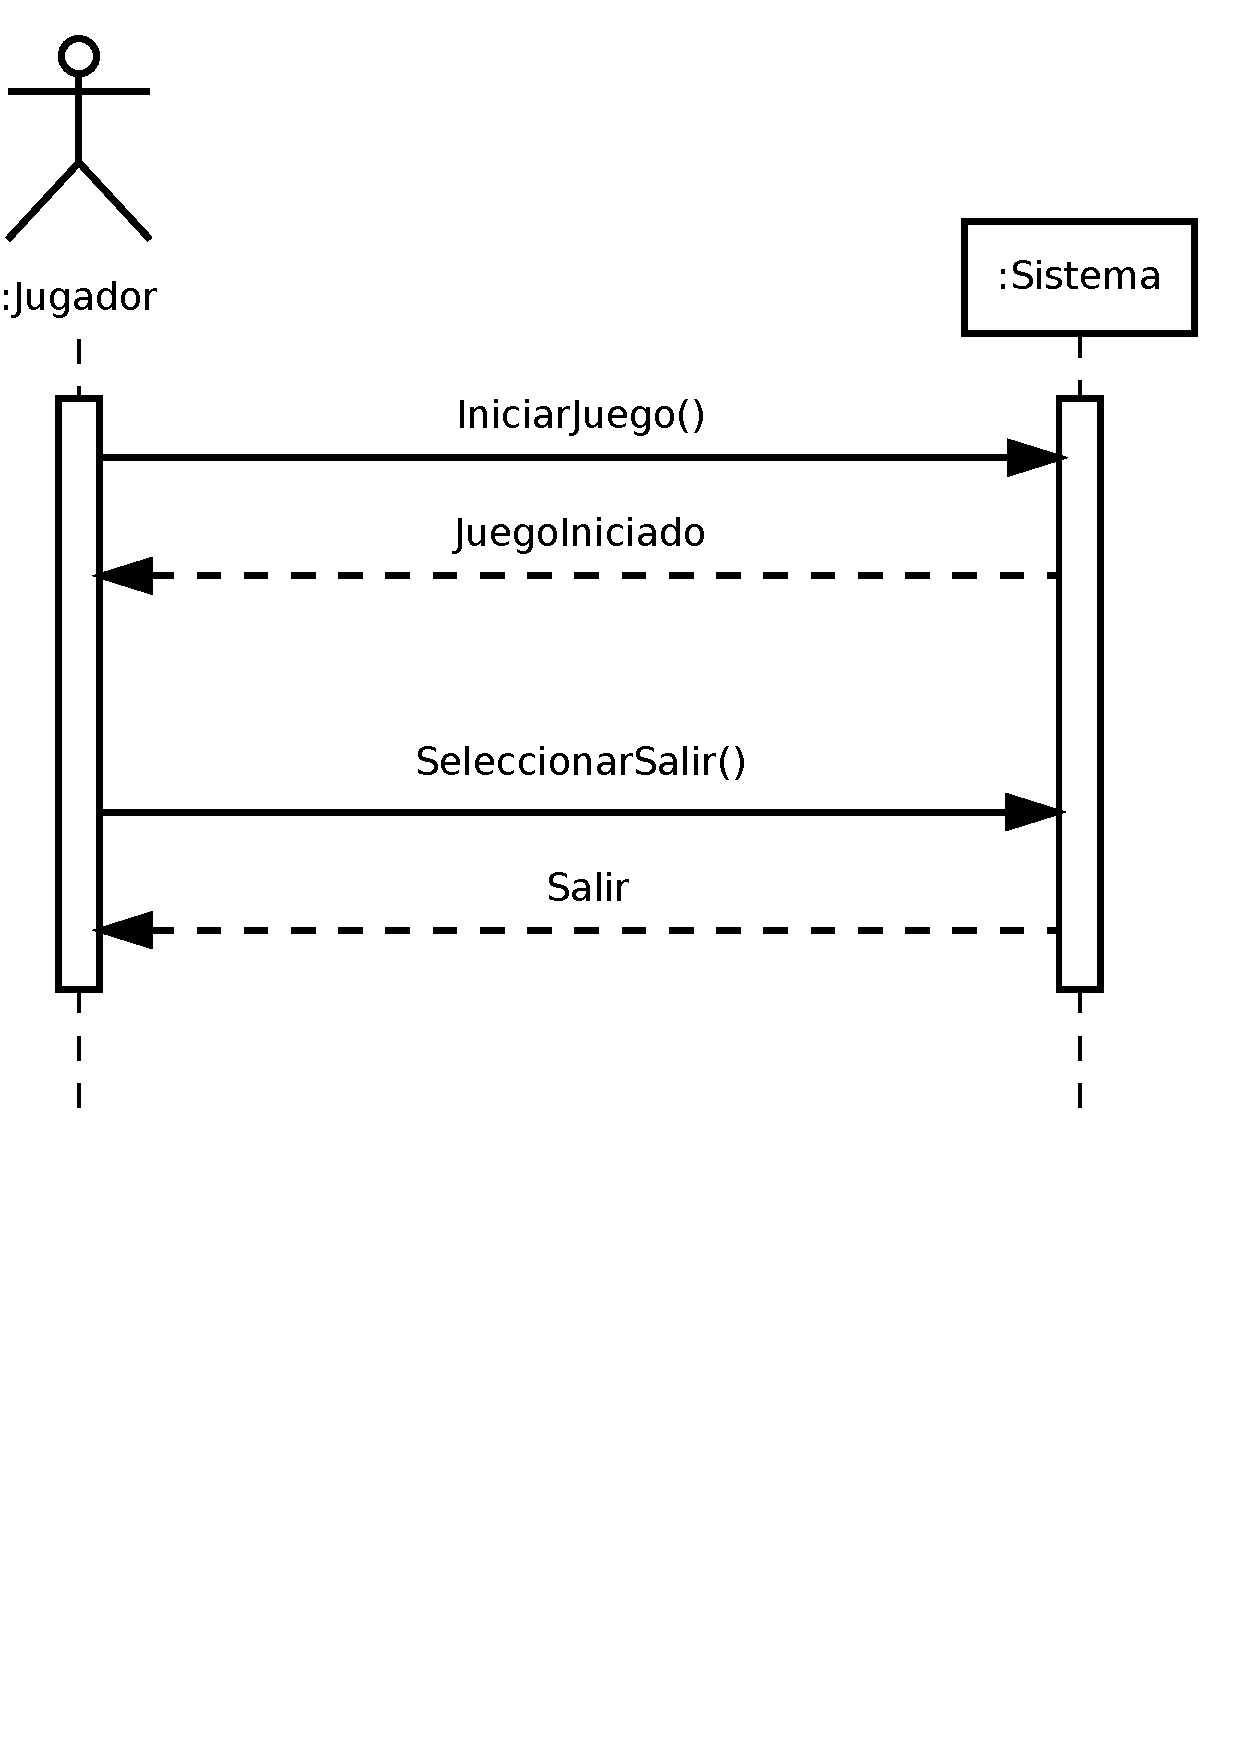
\includegraphics[trim=0cm 12cm 0cm 0cm, clip=true, width=0.5\textwidth]{4_analisis/diagsec_caso1_esc5}
  \caption{Diagrama de secuencia, incio del juego, escenario alternativo 4d}
\end{figure}

\begin{description}
\item[Operación] SeleccionarSalir()
\item[Actores] \jugador\, \sistema\
\item[Responsabilidades] Esconder el menú principal, descargar los recursos y
  cerrar la aplicación.
\item[Precondiciones] $\quad$
  \begin{itemize}
  \item El estado actual es una instancia de \textit{EstadoMenú}.
  \end{itemize}
\item[Postcondiciones] Se destruye el estado \textit{EstadoMenú}, se destruye la
  instancia de la clase \textit{Juego} y termina la ejecución de la aplicación.
\end{description}

\subsection{Selección de canción}

\subsubsection{Escenario principal}
\begin{figure}[h!]
  \centering
  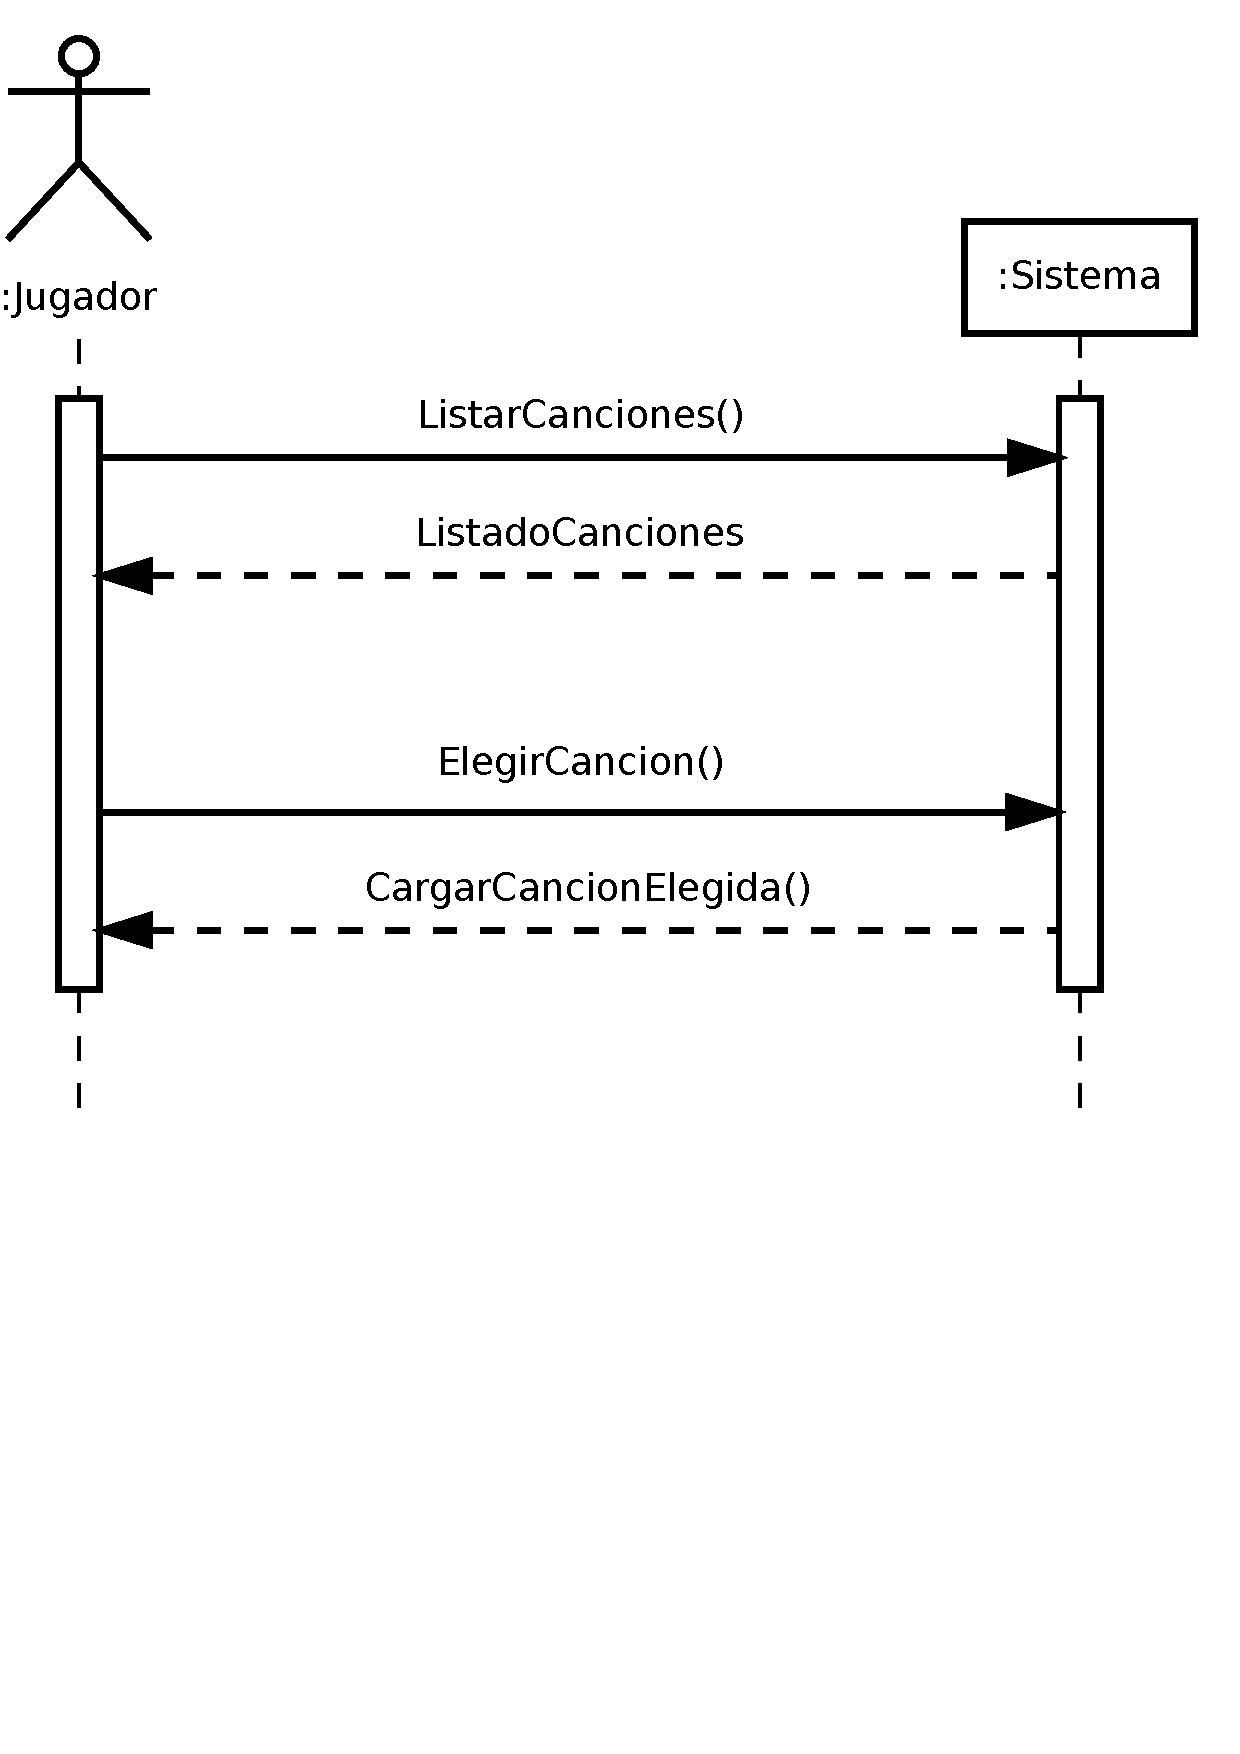
\includegraphics[trim=0cm 12cm 0cm 0cm, clip=true, width=0.5\textwidth]{4_analisis/diagsec_caso2_esc1}
  \caption{Diagrama de secuencia, selección de canción, escenario principal}
\end{figure}

\begin{description}
\item[Operación] ListarCanciones()
\item[Actores] \jugador\, \sistema\
\item[Responsabilidades] Cargar y mostrar la lista de canciones cargadas en el
  sistema.
\item[Precondiciones] Se ordenó la carga del estado \textit{EstadoMenuCanción}
\item[Postcondiciones] $\quad$
  \begin{itemize}
  \item El estado actual es una instancia de \textit{EstadoMenuCanción}.
  \item Se ha cargado la lista de canciones y se muestra en pantalla.
  \end{itemize}
\end{description}

\begin{description}
\item[Operación] ElegirCanción()
\item[Actores] \jugador\, \sistema\
\item[Responsabilidades] Cargar la canción que el usuario ha elegido para
  interpretar.
\item[Precondiciones] Existe una lista de canciones cargada de entre las que el
  usuario ha elegido una.
\item[Postcondiciones] $\quad$
  \begin{itemize}
  \item Se carga la canción indicada.
  \item Se oculta la lista de canciones.
  \item Se pasa a un sub-estado de interpretación de canción.
  \end{itemize}
\end{description}
\subsubsection{Escenario alternativo 3a}
\begin{figure}[h!]
  \centering
  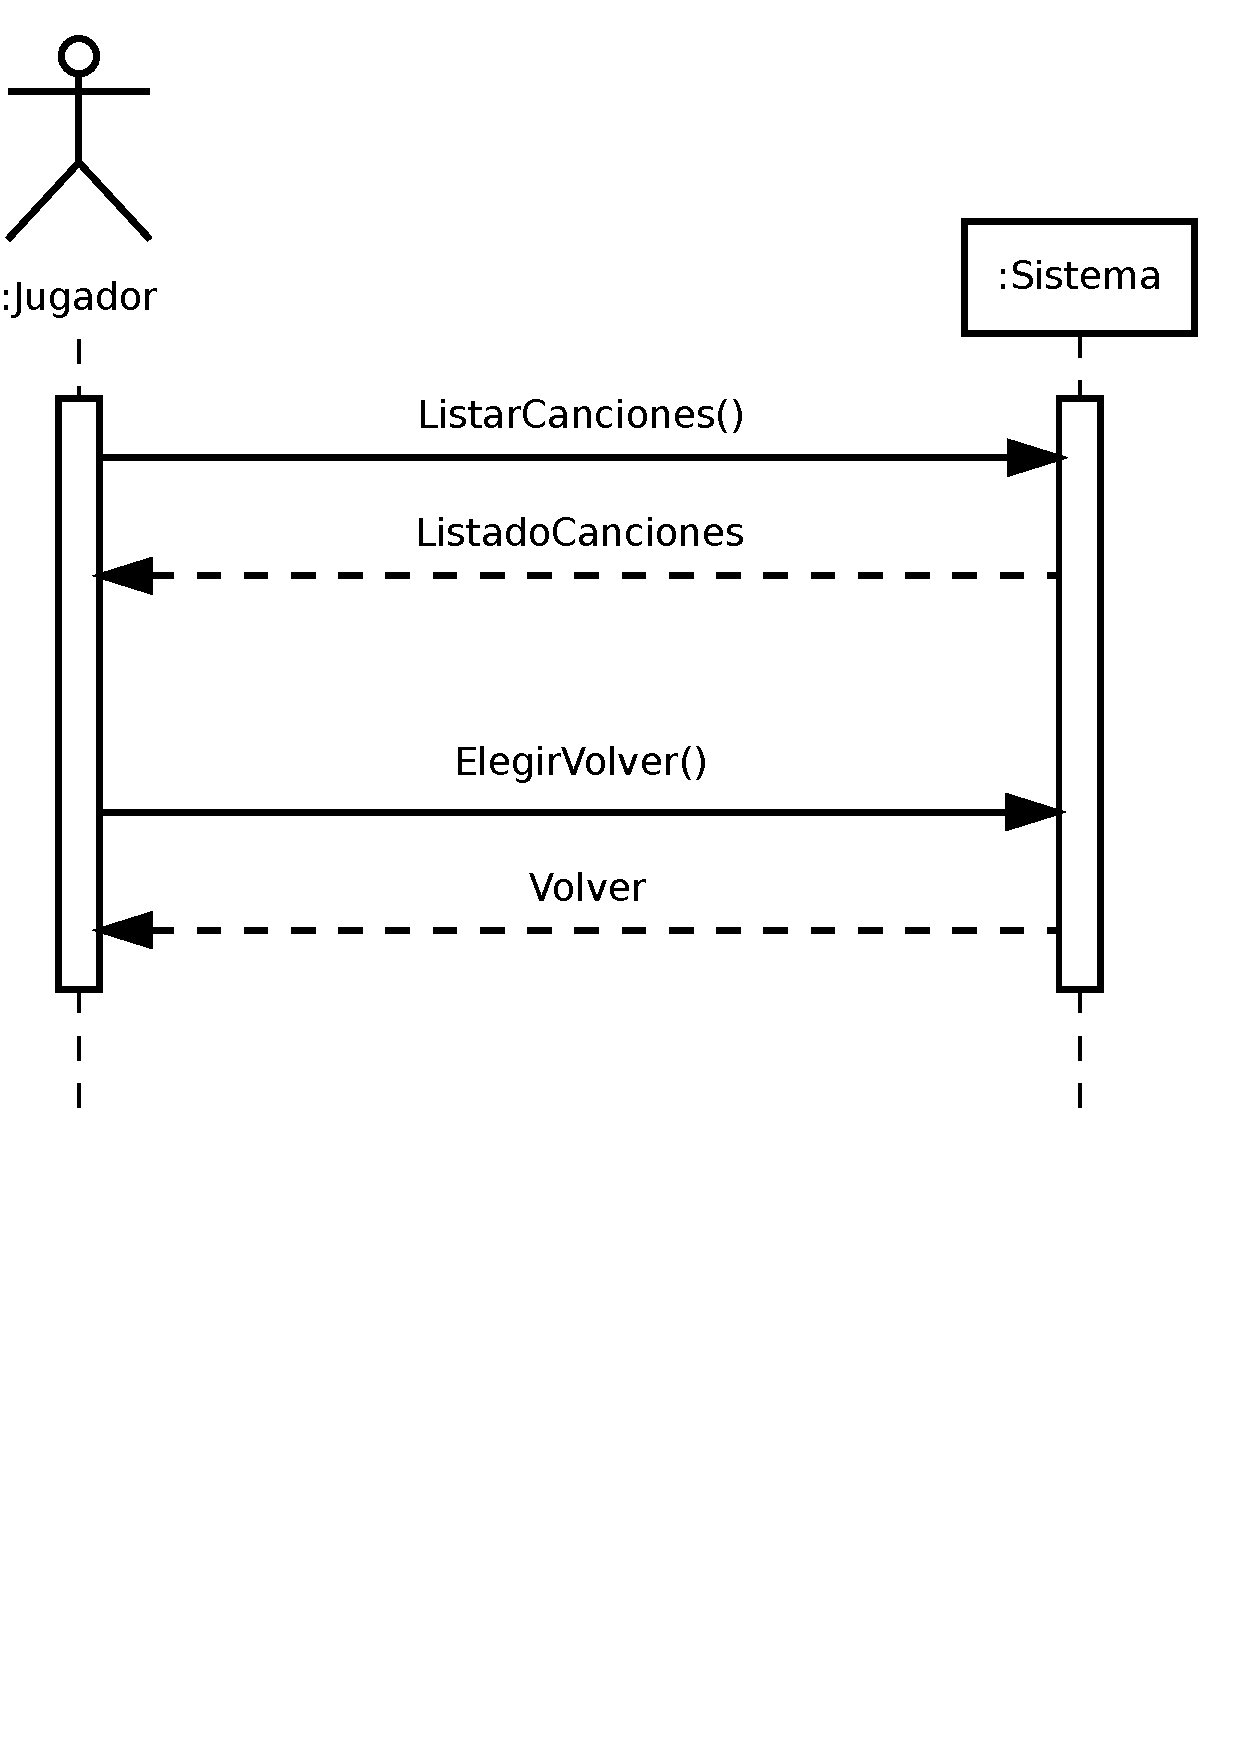
\includegraphics[trim=0cm 12cm 0cm 0cm, clip=true, width=0.5\textwidth]{4_analisis/diagsec_caso2_esc2}
  \caption{Diagrama de secuencia, selección de canción, escenario alternativo 3a}
\end{figure}
\begin{description}
\item[Operación] ElegirVolver()
\item[Actores] \jugador\, \sistema\
\item[Responsabilidades] Descargar la sección actual y volver al menú anterior.
\item[Precondiciones] El estado actual es una instancia de \textit{EstadoMenuCanción}.
\item[Postcondiciones] $\quad$
  \begin{itemize}
  \item El estado instancia de \textit{EstadoMenuCanción} queda descargado.
  \item Se carga y se muestra \textit{EstadoMenú}.
  \end{itemize}
\end{description}

\subsection{Interpretación de canción}
\begin{nota}
  No se reflejan los escenarios alternativos al estar englobados en la operación
  \textit{InteractuarConFlauta}.
\end{nota}

\subsubsection{Escenario principal}
\begin{figure}[h!]
  \centering
  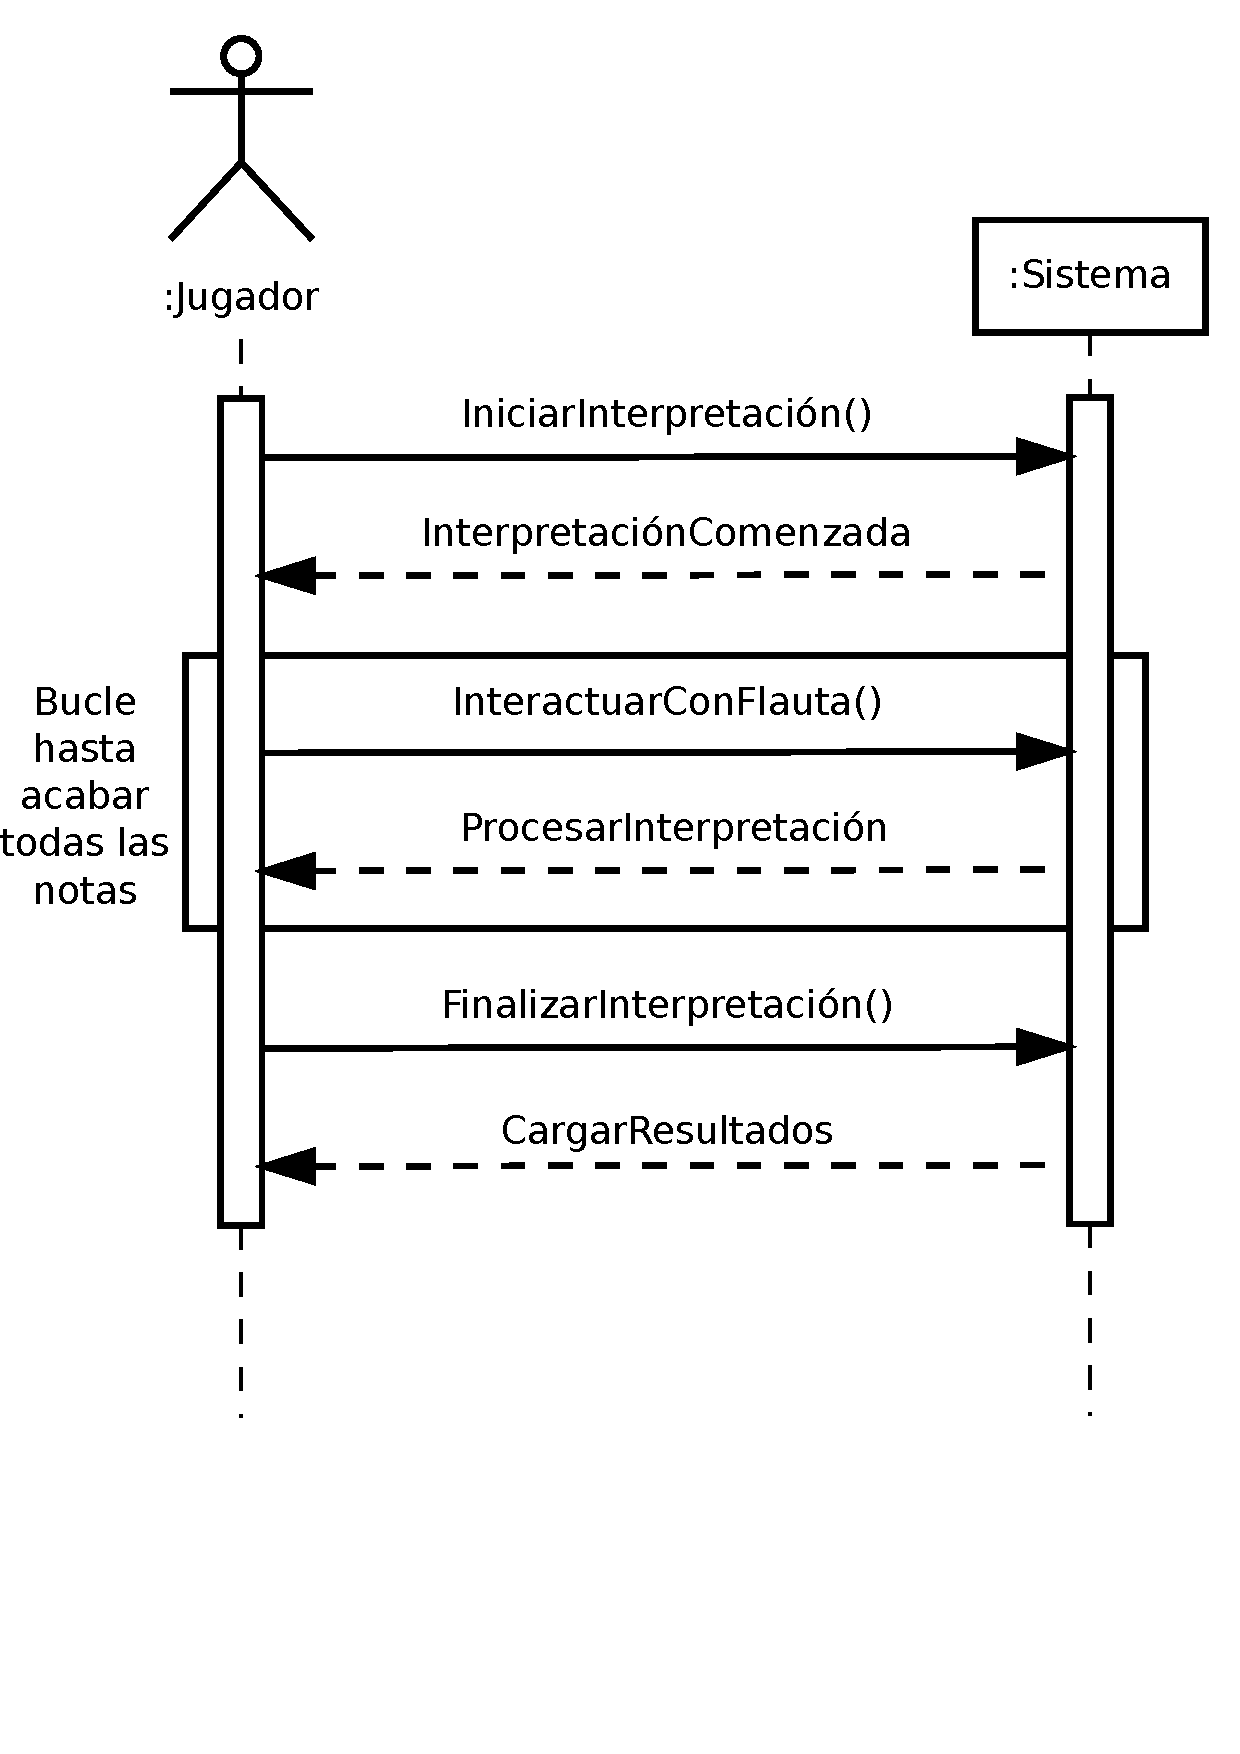
\includegraphics[trim=0cm 8cm 0cm 0cm, clip=true, width=0.5\textwidth]{4_analisis/diagsec_caso3}
  \caption{Diagrama de secuencia, interpretación de canción, escenario principal}
\end{figure}

\begin{description}
\item[Operación] IniciarInterpretación()
\item[Actores] \jugador\, \sistema\
\item[Responsabilidades] Parsear el fichero de canción, cargar la interfaz y
  comenzar la interpretación.
\item[Precondiciones] El usuario ha elegido una canción en el estado anterior.
\item[Postcondiciones] $\quad$
  \begin{itemize}
  \item Se muestra la interfaz de interpretación de canción.
  \item El fichero de canción queda cargado e interpretado, instanciando los
    elementos de la clase \textit{Nota} que sean necesarios.
  \item Comienza la interpretación
  \end{itemize}
\end{description}

\begin{description}
\item[Operación] InteractuarConFlauta()
\item[Actores] \jugador\, \sistema\
\item[Responsabilidades] El \jugador\ interactúa con el sistema mediante la
  flauta a través del micrófono, y el \sistema\ analiza los datos y muestra una
  respuesta en pantalla.
\item[Precondiciones] $\quad$
  \begin{itemize}
  \item La interpretación ha comenzado.
  \item El micrófono está correctamente configurado.
  \end{itemize}
\item[Postcondiciones] $\quad$
  \begin{itemize}
  \item El sistema captura y analiza los datos de audio.
  \item Según el análisis, el sistema responde de una forma u otra (según los
    escenarios alternativos 3a, 4a y 5a del caso de uso \textit{interpretación
      de canción}).
  \end{itemize}
\end{description}

\begin{description}
\item[Operación] FinalizarInterpretación()
\item[Actores] \jugador\, \sistema\
\item[Responsabilidades] Descargar la pantalla de interpretación, descargar la
  canción y finalizar la interpretación.
\item[Precondiciones] Todas las notas se han interpretado.
\item[Postcondiciones] $\quad$
  \begin{itemize}
  \item Se descarga la \textit{Canción} actual.
  \item Se ocultan los elementos de la interfaz de interpretación.
  \item Se lanza la sección de puntuación.
  \end{itemize}
\end{description}


\subsection{Resultados de interpretación}

\subsubsection{Escenario principal}
\begin{figure}[h!]
  \centering
  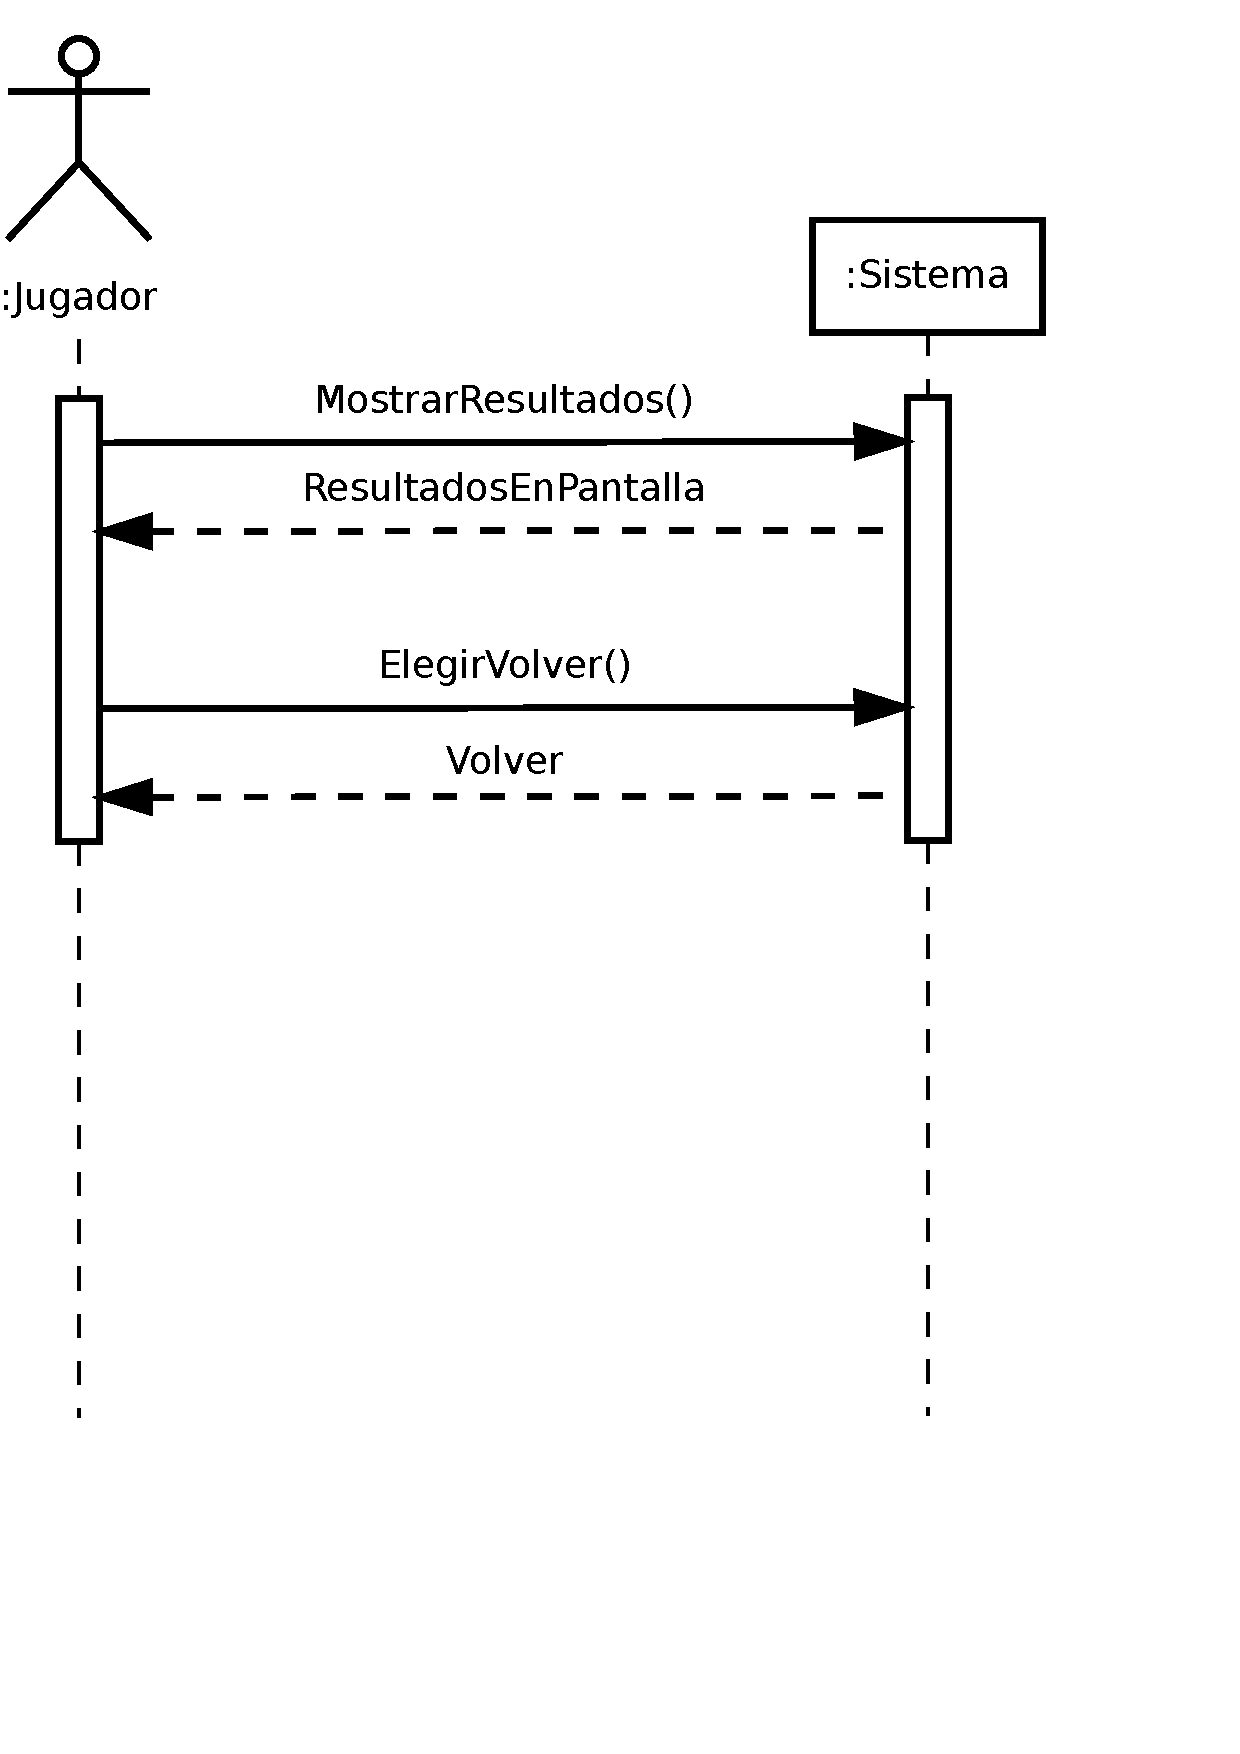
\includegraphics[trim=0cm 12cm 0cm 0cm, clip=true, width=0.5\textwidth]{4_analisis/diagsec_caso4}
  \caption{Diagrama de secuencia, resultados de interpretación, escenario principal}
\end{figure}

\begin{description}
\item[Operación] MostrarResultados()
\item[Actores] \jugador\, \sistema\
\item[Responsabilidades] Interpretar los resultados de la interpretación y
  mostrar los resultados en pantalla.
\item[Precondiciones] El \jugador\ ha concluído satisfactoriamente una
  interpretación completa de una canción, obteniendo una suma de puntos $X$.
\item[Postcondiciones] Mostrar en pantalla los resultados en forma de porcentaje
  de aciertos, y un mensaje según aquél.
\end{description}

\begin{description}
\item[Operación] ElegirVolver()
\item[Actores] \jugador\, \sistema\
\item[Responsabilidades] Descargar la sección actual y volver al menú anterior.
\item[Precondiciones] $\quad$
  \begin{itemize}
  \item La aplicación se encuentra en la pantalla de muestra de resultados.
  \item El usuario ha pulsado la tecla \texttt{escape} o el botón \textit{volver}.
  \end{itemize}
\item[Postcondiciones] $\quad$
  \begin{itemize}
  \item Se descargan todos los datos referentes a la canción actual.
  \item Se carga y se muestra \textit{EstadoMenúCanciones}.
  \end{itemize}
\end{description}

\subsection{Analizador de notas}

\begin{nota}
  No se reflejan los escenarios alternativos al estar englobados en la operación
  \textit{InteractuarConFlauta}.
\end{nota}

\subsubsection{Escenario principal}
\begin{figure}[h!]
  \centering
  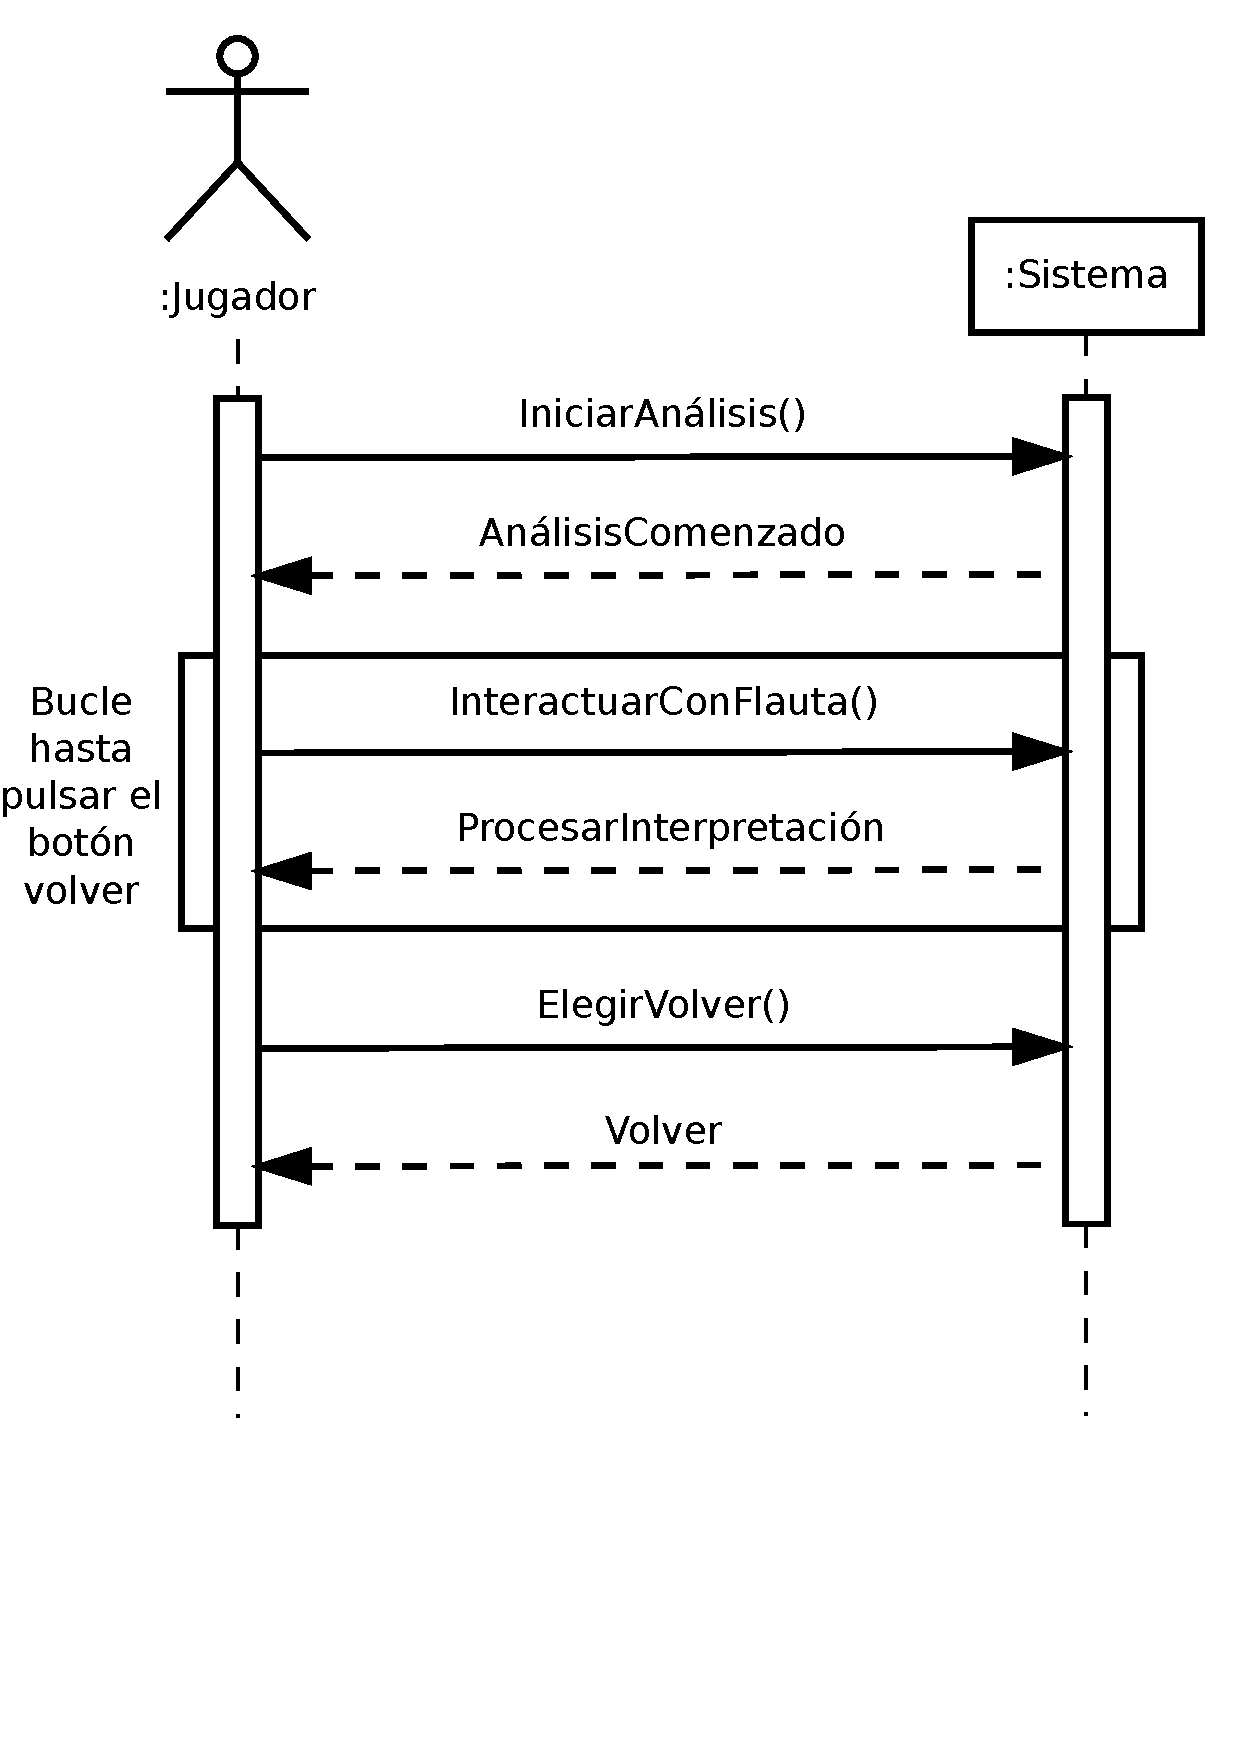
\includegraphics[trim=0cm 8cm 0cm 0cm, clip=true, width=0.5\textwidth]{4_analisis/diagsec_caso5}
  \caption{Diagrama de secuencia, interpretación de canción, escenario principal}
\end{figure}

\begin{description}
\item[Operación] IniciarAnálisis
\item[Actores] \jugador\, \sistema\
\item[Responsabilidades] Cargar la interfaz e iniciar el análisis de notas.
\item[Precondiciones] El usuario eligió la sección \textit{Analizador de notas}
  en el menú principal.
\item[Postcondiciones] $\quad$
  \begin{itemize}
  \item Aparece la interfaz del analizador de notas.
  \item Se inicia el análisis de notas
  \end{itemize}
\end{description}

\begin{description}
\item[Operación] InteractuarConFlauta
\item[Actores] \jugador\, \sistema\
\item[Responsabilidades] El \jugador\ toca notas en la flauta y el \sistema\
  captura y reconoce el audio, indicando la nota tocada en pantalla.

\item[Precondiciones] Se ha iniciado el análisis.

\item[Postcondiciones] $\quad$
  \begin{itemize}
  \item El \sistema\ recoge y analiza el sonido que emite la flauta del \jugador.
  \item El \sistema\ representa en pantalla la nota identificada, o no muestra
    nada en caso de identificación defectuosa.
  \end{itemize}
\end{description}

% \begin{description}
% \item[Operación] ElegirVolver()
% \item[Actores] \jugador\, \sistema\
% \item[Responsabilidades] Descargar la sección actual y volver al menú anterior.
% \item[Precondiciones] $\quad$
%   \begin{itemize}
%   \item El estado actual es una instancia de \textit{EstadoAnalizador}.
%   \item Hay un análisis en curso.  
%   \end{itemize}
  
% \item[Postcondiciones] $\quad$
%   \begin{itemize}
%   \item Concluye el análisis actual.
%   \item Se destruye el estado.
%   \item Se carga y se muestra \textit{EstadoMenú}.
%   \end{itemize}
% \end{description}

\subsection{Calibración de micrófono}

\subsubsection{Escenario principal}
\begin{figure}[h!]
  \centering
  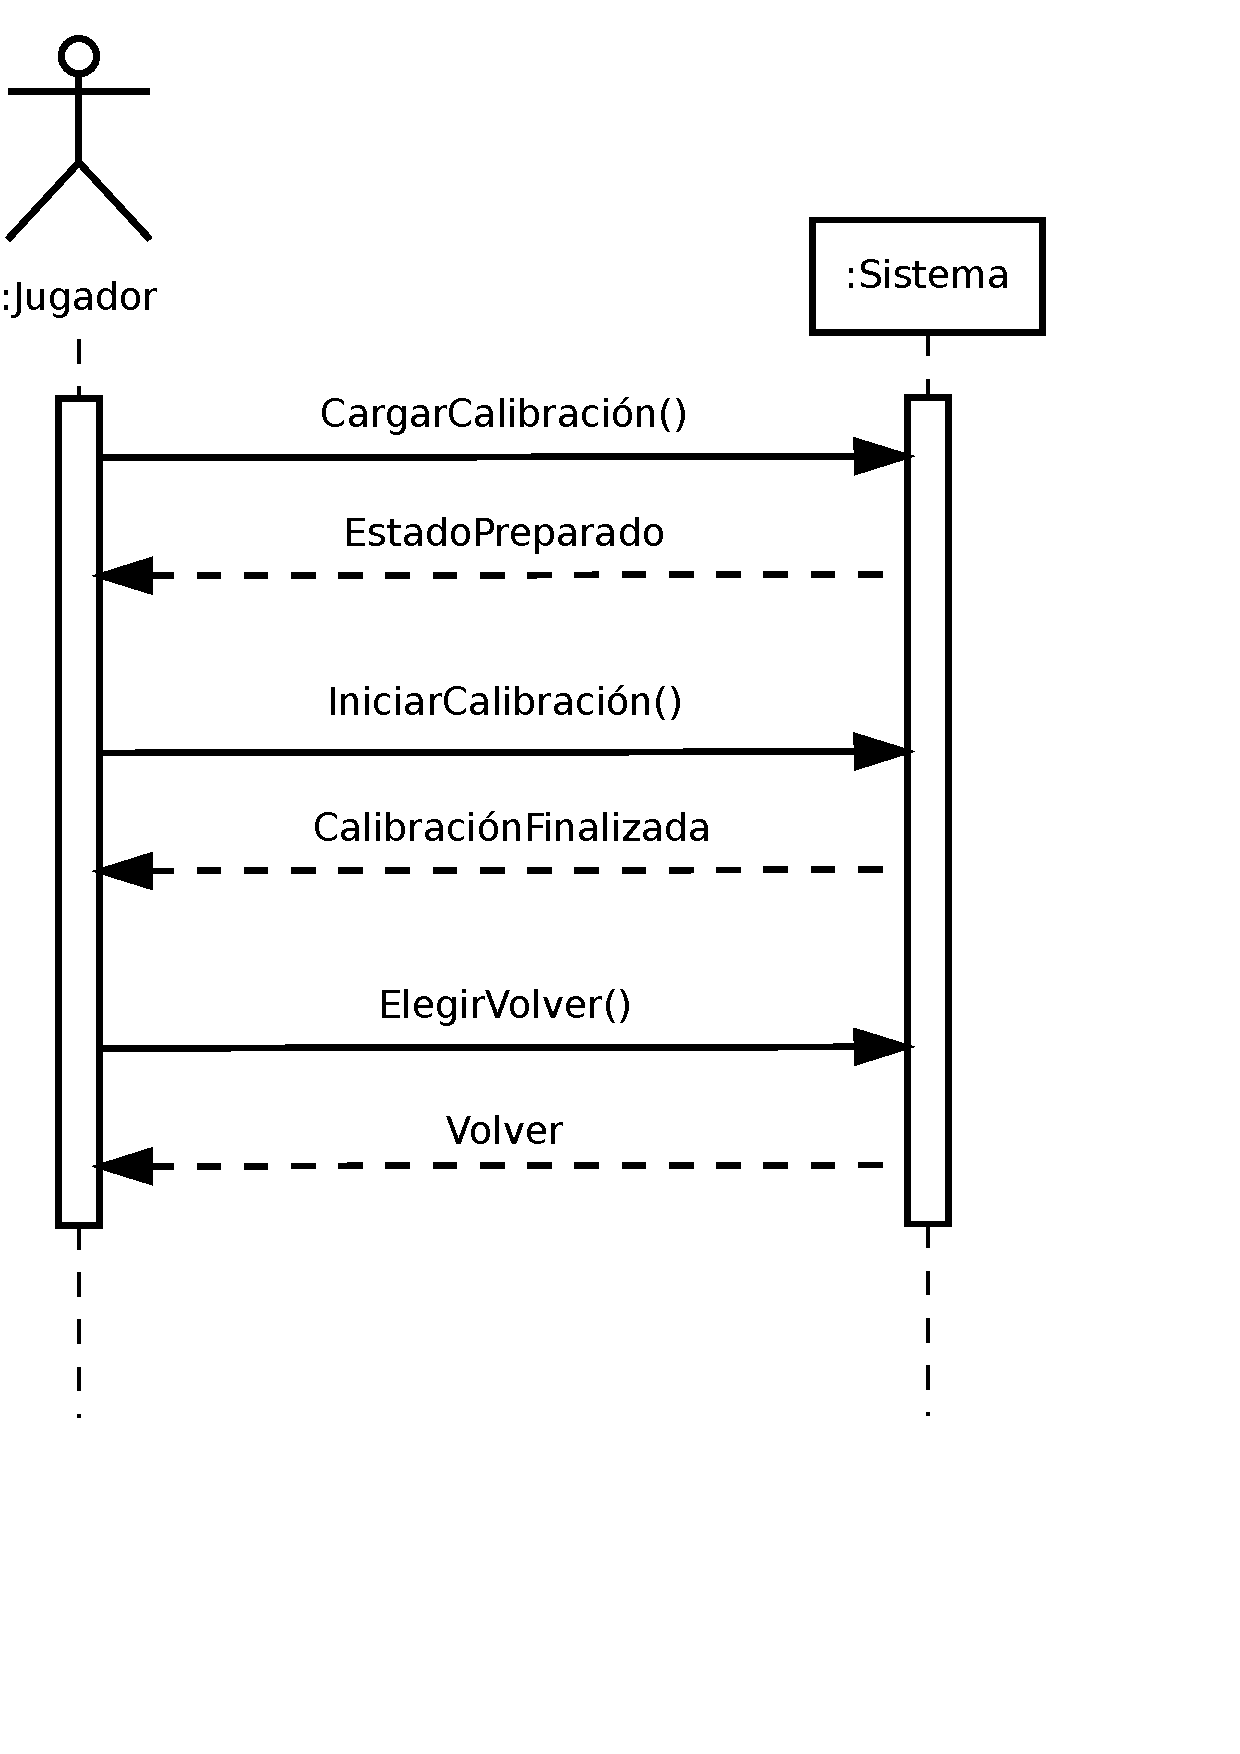
\includegraphics[trim=0cm 8cm 0cm 0cm, clip=true, width=0.5\textwidth]{4_analisis/diagsec_caso6_esc1}
  \caption{Diagrama de secuencia, calibración de micrófono, escenario principal}
\end{figure}

\begin{description}
\item[Operación] CargarCalibración()
\item[Actores] \jugador\, \sistema\
\item[Responsabilidades] Cargar la sección y preparar el sistema para comenzar
  la calibración del micrófono.
\item[Precondiciones] El usuario ha elegido en el menú principal la opción
  \textit{Calibrar micrófono}.
\item[Postcondiciones] La sección está cargada y la calibración lista para
  iniciarse.
\end{description}

\begin{description}
\item[Operación] CalibrarMicrófono()
\item[Actores] \jugador\, \sistema\
\item[Responsabilidades] Llevar a cabo la calibración correcta del micrófono.
\item[Precondiciones] El usuario ha lanzado la calibración del micrófono.
\item[Postcondiciones] $\quad$
  \begin{itemize}
  \item Se cierra el sistema de sonido.
  \item Se obtiene un valor umbral de ruido ambiente, fruto de una calibración
    exitosa.
  \end{itemize}
\end{description}

\begin{description}
\item[Operación] ElegirVolver()
\item[Actores] \jugador\, \sistema\
\item[Responsabilidades] Descargar la sección actual y volver al menú anterior.
\item[Precondiciones] $\quad$
  \begin{itemize}
  \item La calibración ha concluído exitosamente.
  \item El usuario ha pulsado la tecla \texttt{escape} o el botón \textit{volver}.
  \end{itemize}
\item[Postcondiciones] $\quad$
  \begin{itemize}
  \item Se descarga la sección actual.
  \item Se carga y se muestra \textit{EstadoMenúCanciones}.
  \end{itemize}
\end{description}

\subsubsection{Escenario alternativo 5a}
\begin{figure}[h!]
  \centering
  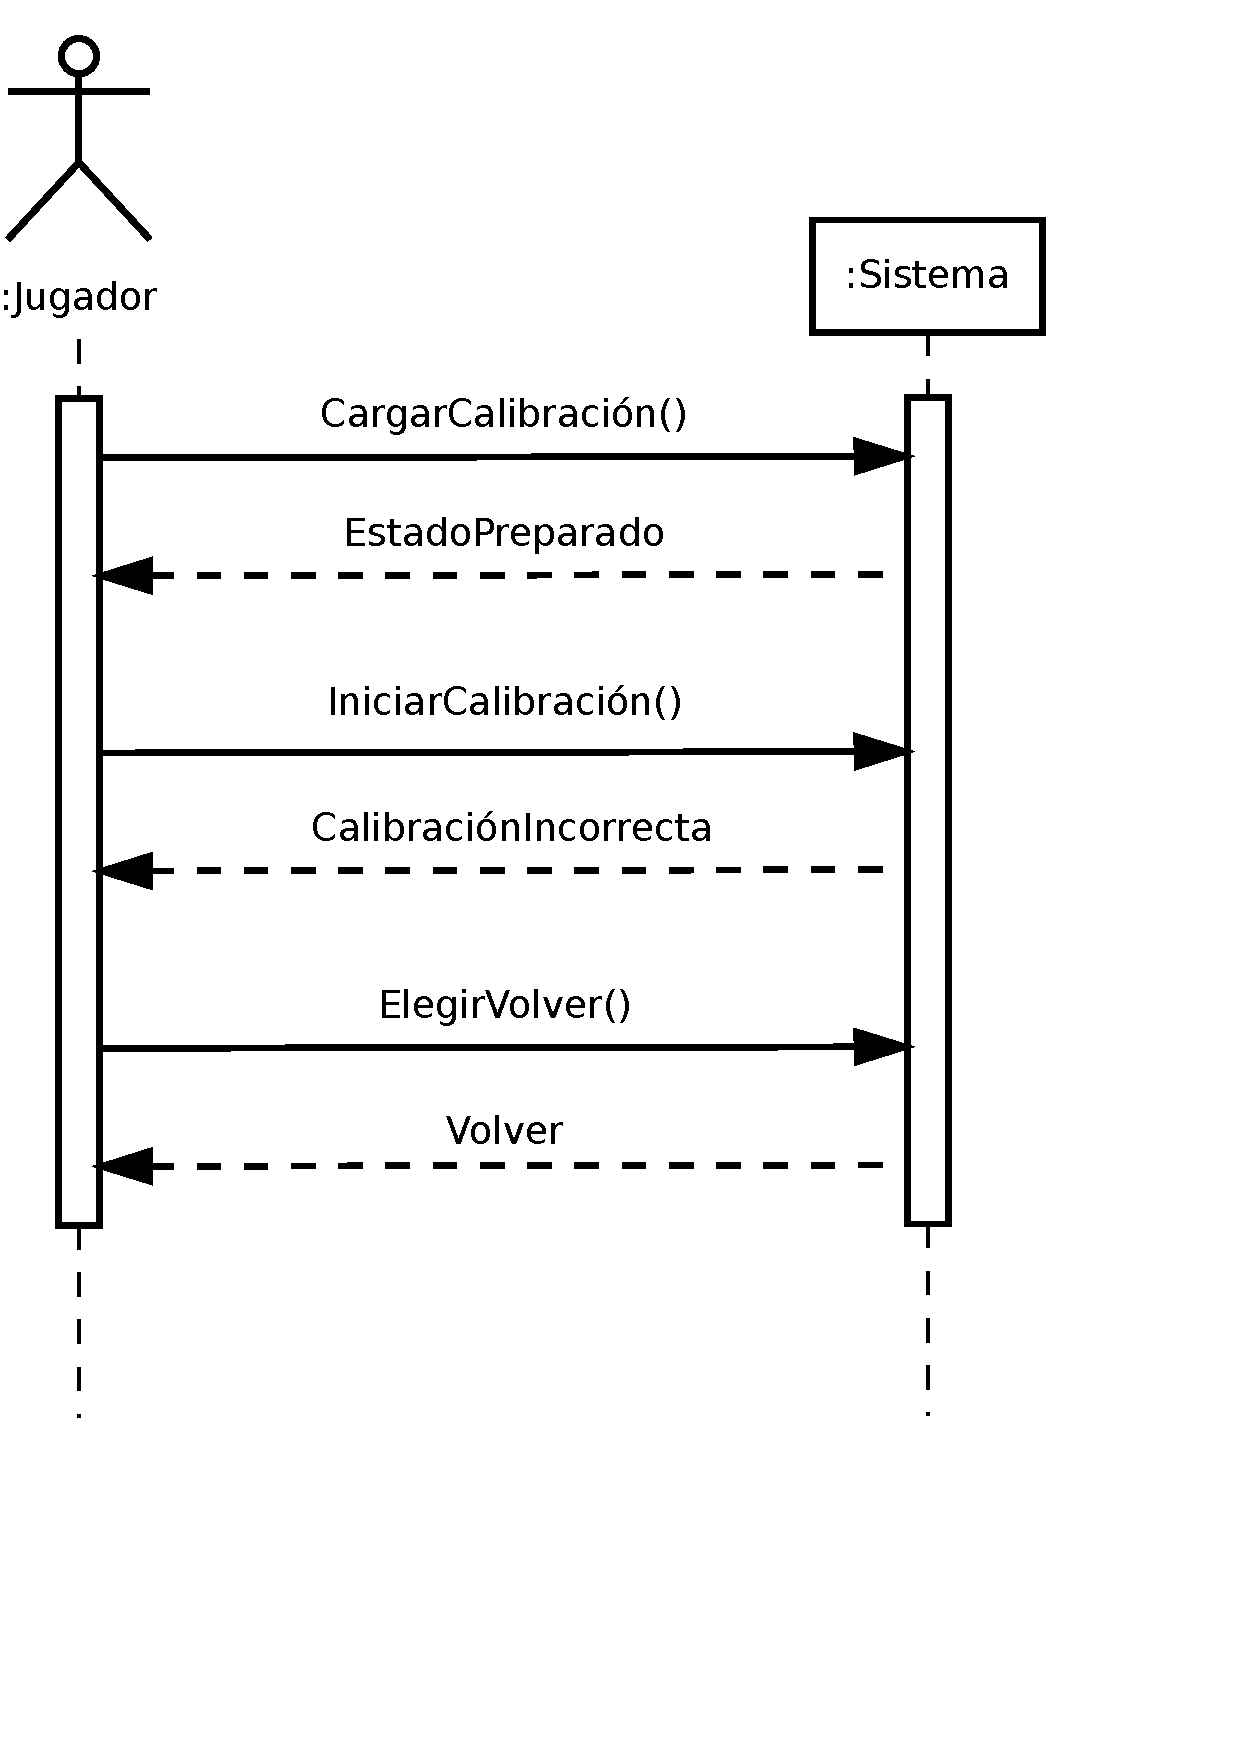
\includegraphics[trim=0cm 8cm 0cm 0cm, clip=true, width=0.5\textwidth]{4_analisis/diagsec_caso6_esc2}
  \caption{Diagrama de secuencia, calibración de micrófono, escenario principal}
\end{figure}
\begin{description}
\item[Operación] CalibrarMicrófono()
\item[Actores] \jugador\, \sistema\
\item[Responsabilidades] Llevar a cabo la calibración correcta del micrófono.
\item[Precondiciones] El usuario ha lanzado la calibración del micrófono.
\item[Postcondiciones] $\quad$
  \begin{itemize}
  \item Se cierra el sistema de sonido.
  \item La calibración ha fallado.
  \item No se obtiene valor umbral de ruido ambiental.
  \end{itemize}
\end{description}

\subsection{Selección de lecciones}

\subsubsection{Escenario principal}
\begin{figure}[h!]
  \centering
  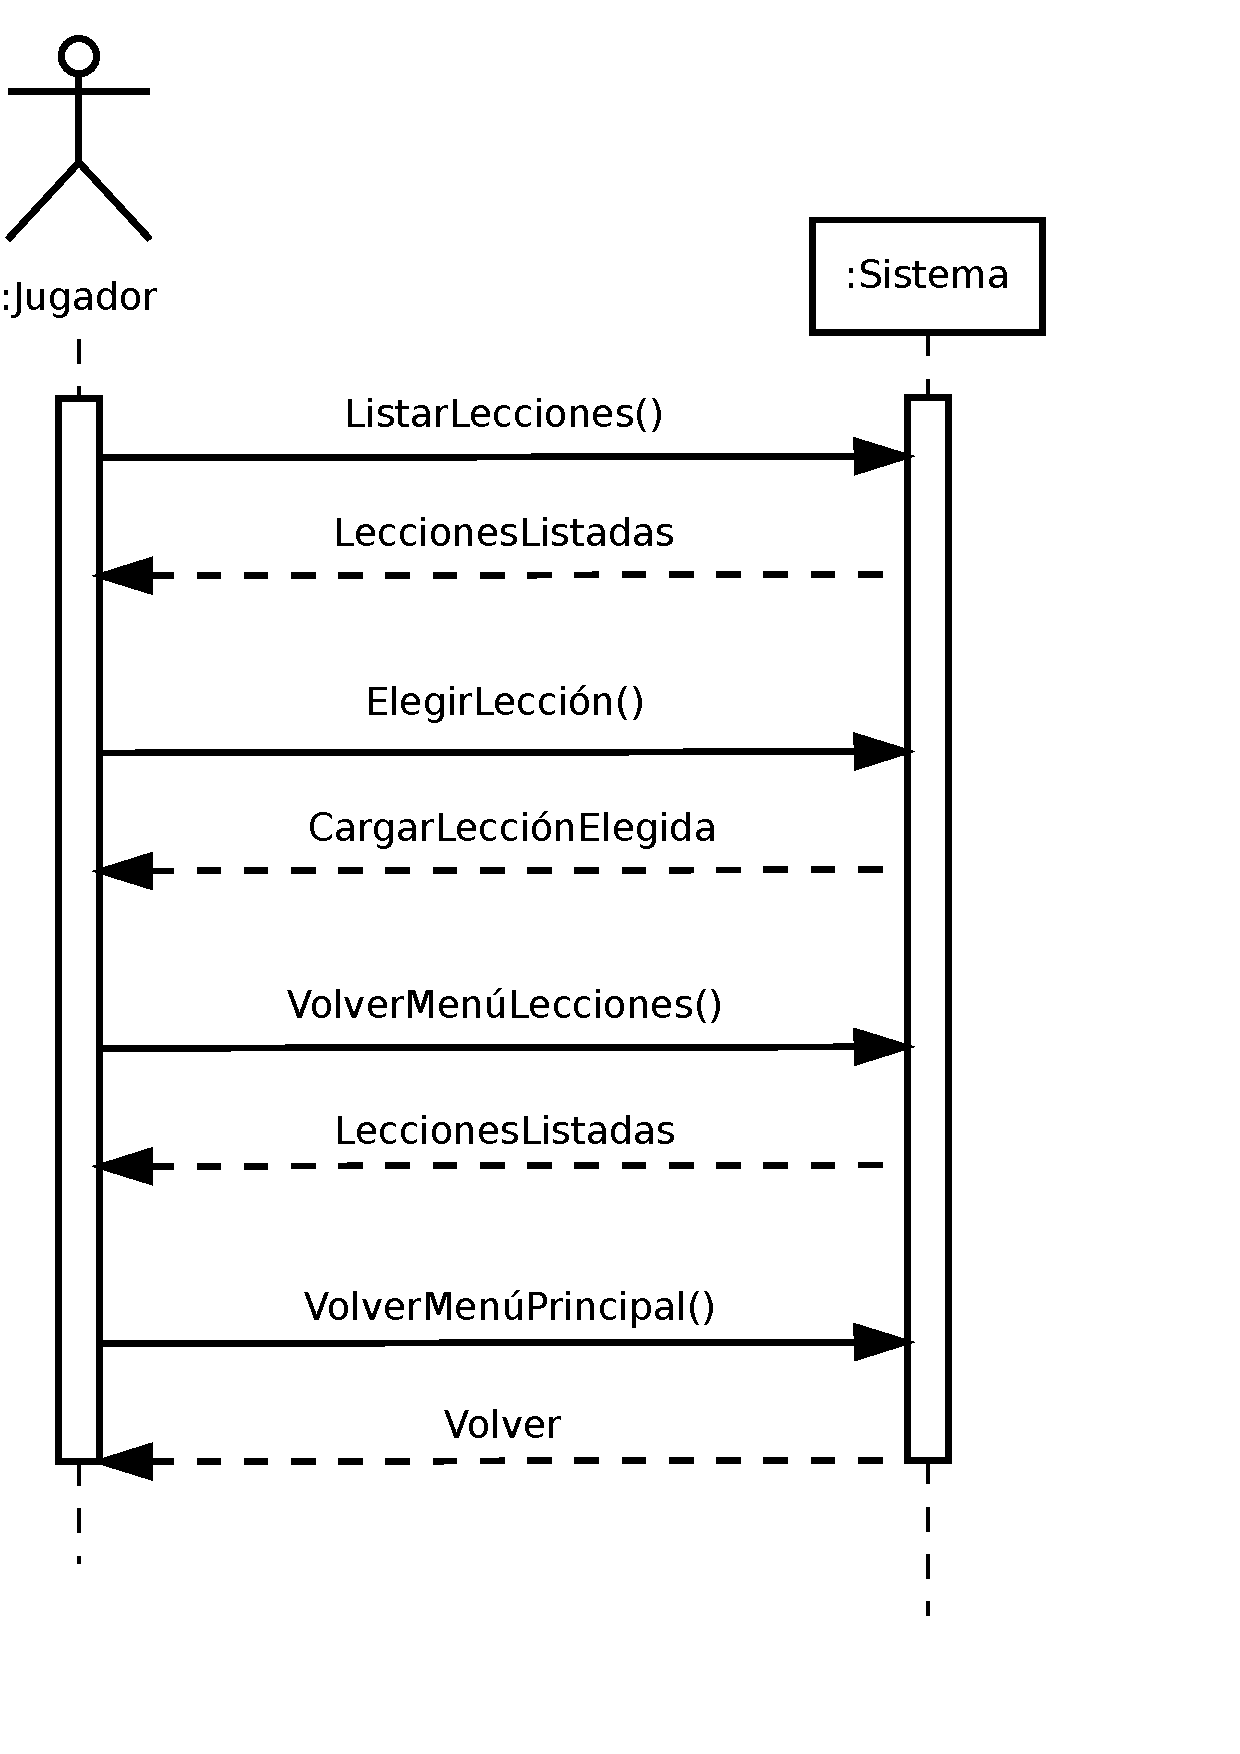
\includegraphics[trim=0cm 4cm 0cm 0cm, clip=true, width=0.5\textwidth]{4_analisis/diagsec_caso7_esc1}
  \caption{Diagrama de secuencia, selección delecciones, escenario principal}
\end{figure}


\begin{description}
\item[Operación] ListarLecciones()
\item[Actores] \jugador\, \sistema\
\item[Responsabilidades] Mostrar el menú de selección de lecciones y listar
  todas las lecciones disponibles.
\item[Precondiciones] El usuario eligió la opción \textit{Lecciones} en el menú
  principal.
\item[Postcondiciones] $\quad$
  \begin{itemize}
  \item Se muestra la interfaz del menú de selección de lecciones.
  \item Se listan las lecciones cargadas en el sistema
  \end{itemize}
\end{description}

\begin{description}
\item[Operación] ElegirLección()
\item[Actores] \jugador\, \sistema\
\item[Responsabilidades] Cargar y mostrar la lección elegida por el usuario.
\item[Precondiciones] El menú de selección de lecciones está cargado y el
  usuario ha elegido una de las lecciones.
\item[Postcondiciones]$\quad$
  \begin{itemize}
  \item Se oculta el menú de selección de lecciones.
  \item Se interpreta el fichero de lección elegido.
  \item Se muestran los elementos multimedia pertenecientes a la lección
    elegida.
  \end{itemize}
\end{description}

\begin{description}
\item[Operación] VolverMenuLecciones()
\item[Actores] \jugador\, \sistema\
\item[Responsabilidades] Descargar la lección actual y volver al menú anterior.
\item[Precondiciones] $\quad$
  \begin{itemize}
  \item El usuario ha terminado de ver la lección elegida.
  \item El usuario ha pulsado la tecla \texttt{escape} o el botón \textit{volver}.
  \end{itemize}
\item[Postcondiciones] $\quad$
  \begin{itemize}
  \item Se descarga la lección actual.
  \item Se muestra de nuevo el menú de selección de lecciones.
  \end{itemize}
\end{description}

\begin{description}
\item[Operación] VolverMenuPrincipal()
\item[Actores] \jugador\, \sistema\
\item[Responsabilidades] Descargar el menú de selección de lecciones y volver al
  menú principal.
\item[Precondiciones] El usuario ha pulsado la tecla \texttt{escape} o el botón \textit{volver}.
\item[Postcondiciones] $\quad$
  \begin{itemize}
  \item Se descarga el menú de selección de lecciones.
  \item Se carga y muestra el menú principal
  \end{itemize}
\end{description}

\subsubsection{Escenario alternativo}
\begin{figure}[h!]
  \centering
  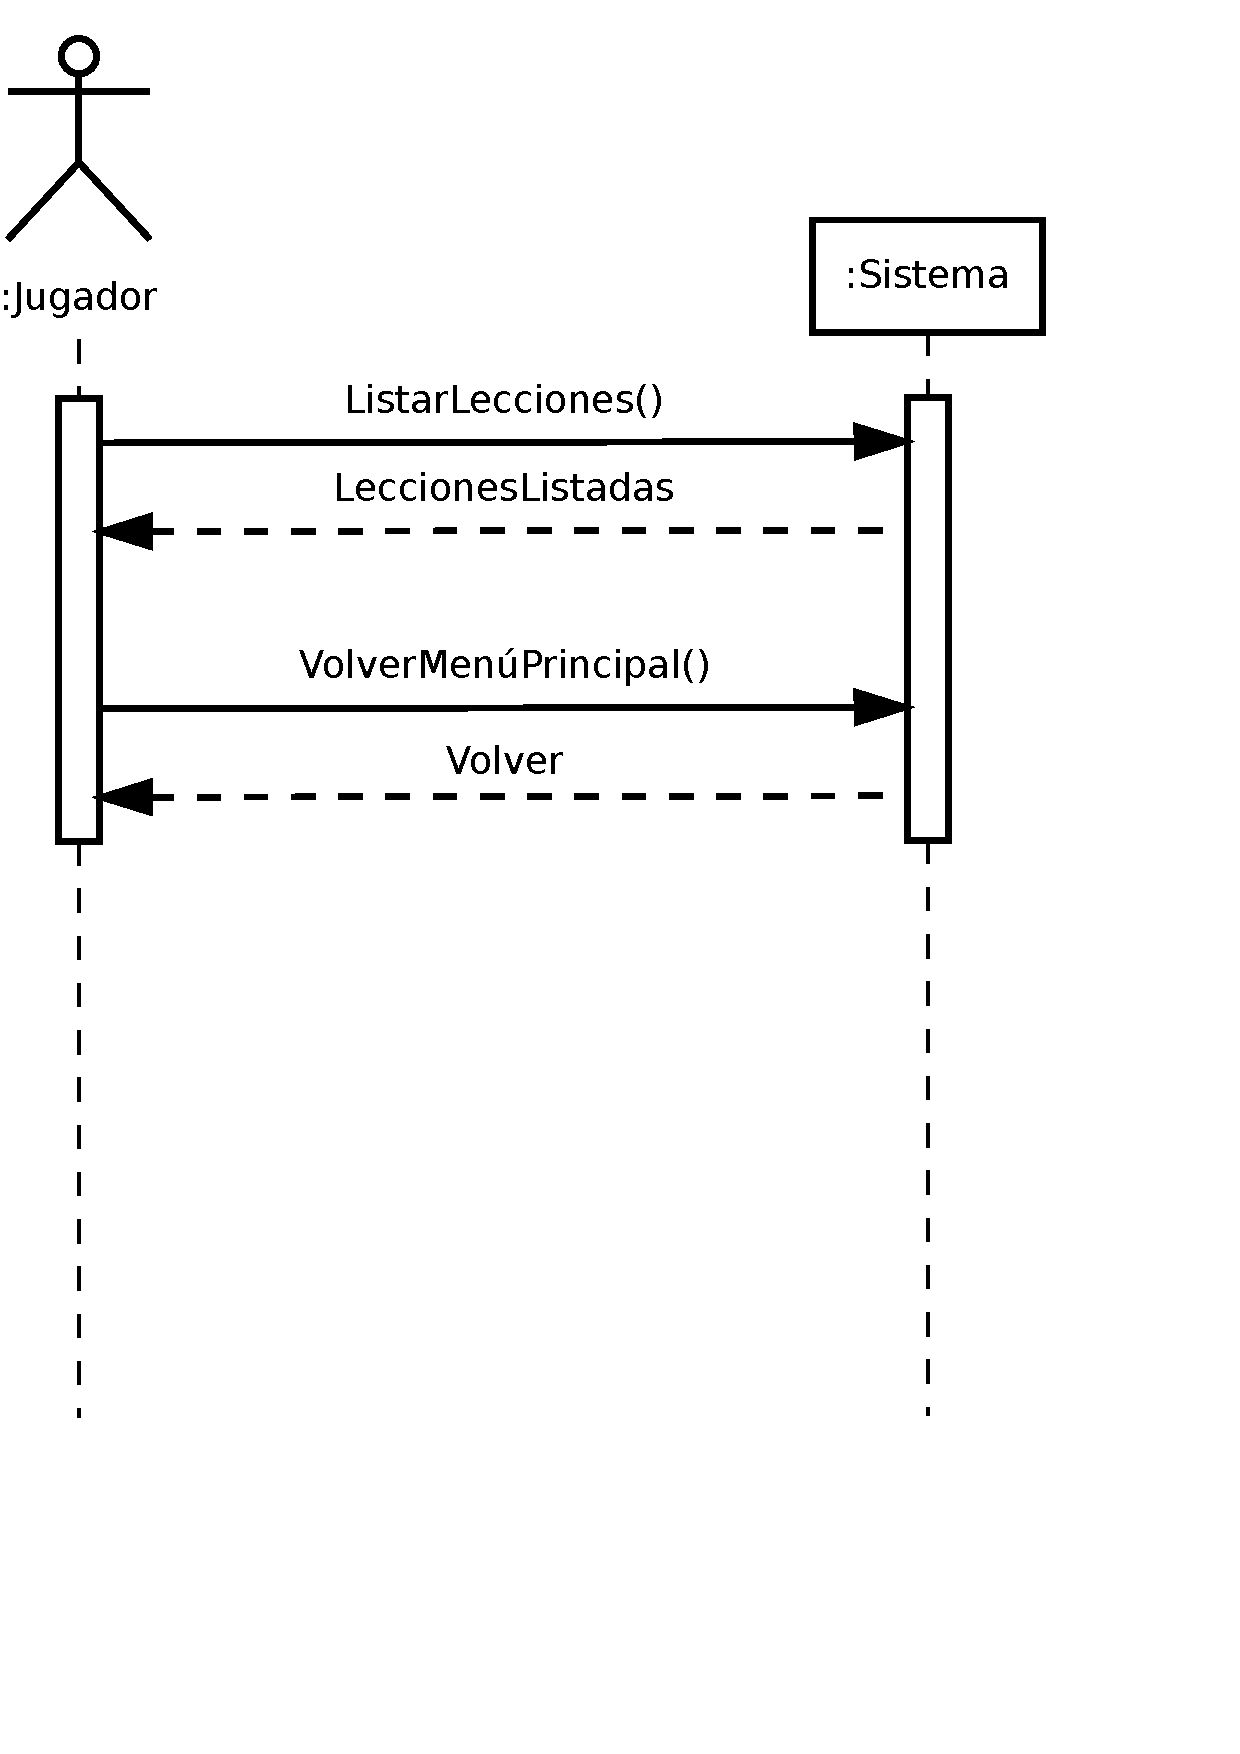
\includegraphics[trim=0cm 12cm 0cm 0cm, clip=true, width=0.5\textwidth]{4_analisis/diagsec_caso7_esc2}
  \caption{Diagrama de secuencia, selección de lecciones, escenario alternativo}
\end{figure}

\begin{description}
\item[Operación] ListarLecciones()
\item[Actores] \jugador\, \sistema\
\item[Responsabilidades] Mostrar el menú de selección de lecciones y listar
  todas las lecciones disponibles.
\item[Precondiciones] El usuario eligió la opción \textit{Lecciones} en el menú
  principal.
\item[Postcondiciones] $\quad$
  \begin{itemize}
  \item Se muestra la interfaz del menú de selección de lecciones.
  \item Se listan las lecciones cargadas en el sistema
  \end{itemize}
\end{description}

\begin{description}
\item[Operación] VolverMenuPrincipal()
\item[Actores] \jugador\, \sistema\
\item[Responsabilidades] Descargar el menú de selección de lecciones y volver al
  menú principal.
\item[Precondiciones] El usuario ha pulsado la tecla \texttt{escape} o el botón \textit{volver}.
\item[Postcondiciones] $\quad$
  \begin{itemize}
  \item Se descarga el menú de selección de lecciones.
  \item Se carga y muestra el menú principal
  \end{itemize}
\end{description}

%%% Local Variables: 
%%% mode: latex
%%% TeX-master: "../memoria"
%%% End: 

%%% Local Variables: 
%%% mode: latex
%%% TeX-master: "../memoria"
%%% End: 


\chapter{Diseño}
wtf

%%% Local Variables: 
%%% mode: latex
%%% TeX-master: "../memoria"
%%% End: 


\chapter{Implementación}
Un análisis claro y un diseño conciso no garantizan que, a la hora de
implementar el sistema planteado, no se encuentre ninguna dificultad o
imprevisto. Así pues, en este capítulo comentaremos los retos y detalles que más
relevancia o complejidad han presentado durante la fase de la implementación del
proyecto.

De igual modo, durante el desarrollo de la aplicación se mantuvo actualizada una
bitácora, accesible en línea~\cite{ofluteblog}, en la que se fueron detallando,
a medida que aparecían, muchas de estas dificultades.

Como complemento a la lectura de este capítulo se recomienda tener una copia
local del repositorio del proyecto, disponible para su libre descarga desde la
forja oficial~\cite{ofluteforja}. En él se encuentra todo el código fuente
original, así como la documentación en formato \textit{Doxygen}~\cite{doxygen}.

\section{Carga y uso de fuentes TrueType en Gosu}

Como se ha comentado previamente, \textbf{oFlute} hace uso de la biblioteca
\textit{Gosu}, que proporciona una API sencilla para el acceso al sistema
gráfico, entre otras características. Este framework funciona en sistemas
Windows, GNU/Linux y Mac OS, aunque dada la dificultad de conseguir la
compatibilidad con todos ellos, la calidad y el rendimiento es bastante
desigual de un sistema a otro.

Una de estas desigualdades se presentaba a la hora de \textbf{cargar fuentes}
para mostrar textos. En su versión para GNU/Linux, el módulo para el pintado de
textos de Gosu (que comprende la clase \texttt{Gosu::Font} y las funciones
\texttt{Gosu::drawText} y \texttt{Gosu::createText}) solo permitía
utilizar fuentes que estuvieran ya instaladas en el sistema de forma global, de
modo que era imposible adjuntar un fichero con una fuente en formato
\texttt{TrueType}~\cite{reftruetype} para su carga en el juego. 

La instalación de fuentes en sistemas GNU/Linux siempre ha sido una operación
engorrosa que ha requerido permisos de administrador. Esto, unido a que tanto en
Windows como en Mac OS la opción de cargar fuentes desde un fichero sí estaba
disponible, supuso un grave problema en el planteamiento del proyecto.

Inicialmente se investigaron las razones de esta limitación. Al ser un proyecto
libre y abierto, revisamos el código de Gosu, concretamente la implementación
de la clase \texttt{Gosu::Font} previamente citada, de la que dependían todas
las otras funciones relacionadas con fuentes.

Las conclusiones que se sacaron fueron que Gosu, bajo GNU/Linux, implementaba el
renderizado de fuentes mediante una biblioteca llamada Pango~\cite{Pango}, de
bastante bajo nivel, y que por diseño está limitada al uso de fuentes de
sistema, ya que se orienta a herramientas del sistema operativo, no a
aplicativos de terceros.

Así pues, era necesario buscar una alternativa. En numerosos proyectos
previos~\cite{robinson} se había utilizado la biblioteca
\textbf{SDL}~\cite{refsdl}, un framework multimedia muy utilizado en
aplicaciones de audio, vídeo y juegos. Uno de los subsistemas que proporciona
SDL es \textbf{SDL\_ttf}~\cite{refsdlttf}, una biblioteca para el renderizado de
fuentes basadas en ficheros \texttt{TrueType}. Esto, unido a que la propia SDL
ya era una dependencia de Gosu, propició que se iniciara la implementación de
una solución basada en este medio.

\subsection{Funcionamiento de \texttt{SDL\_ttf}}

Para comprender cómo se implementó la solución al problema citado, el primer
paso es entender cómo funciona la biblioteca \texttt{SDL\_ttf} para poder ver
cómo se corresponde luego con Gosu.

\subsubsection{Tipos de datos utilizados}

En común con el resto de módulos de SDL, SDL\_ttf se basa en un tipo de datos
conocido como \textit{superficies} (\texttt{SDL\_Surface}). Estas superficies
representan mapas de bits cargados en memoria, y se utilizan para guardar las
imágenes que se cargan de los ficheros, así como para representar otros destinos
gráficos intermedios, como la propia pantalla.

Para representar el color del texto que vamos a pintar, SDL\_ttf utiliza la
estructura \texttt{SDL\_Color}, que guardará los valores de color de 8 bits para
los tres canales de color primario (rojo, verde y azul).

Además, SDL\_ttf define un tipo de datos propio, de nombre \texttt{TTF\_Font}, que
representa una fuente cargada a partir de un fichero, con un tamaño determinado.

\subsubsection{Funciones utilizadas}

SDL\_ttf precisa de una \textbf{inicialización} previa, que se lleva a cabo mediante la
llamada a \texttt{TTF\_Init()}. Igualmente, liberaremos los recursos ocupados
mediante \texttt{TTF\_Quit()}.

Para \textbf{cargar la fuente} a partir de los ficheros TrueType (con extensión
\texttt{.ttf}), se utiliza la función \texttt{TTF\_OpenFont(const char * fichero,
  int tamaño)}. Esta función recibe una cadena con el nombre del fichero y el
tamaño de letra a utilizar, y devuelve un puntero al tipo \texttt{TTF\_Font}.

\begin{minted}{cpp}
  TTF_Font * fuente = TTF_OpenFont("fichero_fuente.ttf", 25);
\end{minted}

Una vez cargada la fuente de nuestro interés, tendremos que \textbf{generar una
  superficie} con el texto que queramos. Para ello, SDL\_ttf ofrece una gran
variedad de funciones, según el suavizado del texto y el tipo de caracteres que
estemos utilizando. En nuestro caso, queríamos que la superficie tuviera fondo
transparente, así como usar caracteres en UTF-8~\cite{refutf8}, por lo que la
función que se eligió fue 
\begin{minted}{cpp}
  SDL_Surface * TTF_RenderUTF8_Blended (TTF_Font * fuente,
                                        const char * texto,
                                        SDL_Color color);
\end{minted}

Esta función devolverá un puntero a una superficie que se integrará
(\textit{blends}) sobre cualquier imagen, al tener el fondo transparente.


\subsection{Representación de imágenes en Gosu}

Una vez conocidos los tipos de datos y funciones que ofrece SDL\_ttf, es
necesario conocer cuáles son los tipos de datos equivalentes en Gosu, de forma
que pueda haber una \textit{conversión} de un tipo a otro.

\subsubsection{Mapas de bits de bajo nivel: Gosu::Bitmap}
La clase \texttt{Gosu::Bitmap} representa, en Gosu, un mapa de bits de bajo
nivel. Éste no contará con aceleración por hardware ni podrá mostrarse en
pantalla, pero podremos acceder directamente a los datos de los píxeles y
trabajar con ellos.

\texttt{Gosu::Bitmap} nos servirá de paso intermedio entre la superficie de SDL y las
imágenes habituales de Gosu.

\subsubsection{Imágenes de uso común: Gosu::Image}
En Gosu las imágenes y assets gráficos se manejan habitualmente con la clase
\texttt{Gosu::Image}, que representa un contenedor de más alto nivel que
\texttt{Gosu::Bitmap}, además de estar optimizado y poder pintarse en pantalla.

Podremos crear un objeto de esta clase a partir de un \texttt{Gosu::Bitmap}, consiguiendo
finalmente un objeto \textit{pintable}.


\subsection{Implementación final}

Conocidas las representaciones internas de ambas bibliotecas, se implementó una
clase con una interfaz similar a \texttt{Gosu::Font}, de modo que la transición
pudiera ser lo más transparente posible, de nombre \texttt{CustomFont}.

En el constructor se inicializa (de forma única, mediante una variable estática)
el subsistema \texttt{SDL\_ttf} utilizando la llamada
\texttt{TTF\_Init()}. Después, se carga la fuente indicada por los parámetros
del constructor. En ambos casos, se comprueba que el procedimiento ha sido
correcto, lanzando una excepción en caso contrario.

\begin{minted}{cpp}
static int initResult = TTF_Init();
if (initResult < 0)
   throw std::runtime_error("Could not initialize SDL_TTF");

font = TTF_OpenFont(fontName, fontHeight);
if (!font)
   throw std::runtime_error("Could not open TTF file " + fontName);

\end{minted}

Seguidamente, en el método de pintado (\texttt{draw}) se genera la superficie
con el texto que se indique, pasando el contenido de los píxeles a un contenedor
\texttt{Gosu::Bitmap} y finalmente generando un objeto \texttt{Gosu::Image} a
partir del mismo.

\begin{minted}{cpp}
SDL_Surface * surf = TTF_RenderUTF8_Blended(font, text, color);
if (!surface)
   throw std::runtime_error("Could not generate the surface");

Gosu::Bitmap temp;
temp.resize(surf.width(), surf.height());
std::memcpy(temp.data(), surf.data(), temp.width() * temp.height() * 4);

Gosu::Image image (graphic_target, temp);
image.draw(x, y, z);
\end{minted}

\subsection{Mejora de rendimiento}
Con la implementación anterior, en cada fase de dibujado se tenía que repetir el
proceso completo, aún cuando el texto no cambiase. Esto suponía una pérdida de
rendimiento considerable, sobre todo a la hora de hacer el \textit{trasvase} de
píxeles de la superficie de \texttt{SDL} al mapa de bits de Gosu.

La solución que se utilizó se basó en las implementaciones previas de la clase
\texttt{Gosu::Font}. La idea principal es utilizar un búffer de imágenes para
cada uno de los glifos de la fuente, que se iría rellenando a medida que fuera
necesario pintar cada caracter. Posteriormente, se utilizarían las imágenes en
ese búffer para pintar el texto indicado.

Así, por ejemplo, si en primer lugar se pide pintar el texto \textit{``Score''},
se renderizarían los caracteres \textit{'S'}, \textit{'c'}, \textit{'o'},
\textit{'r'} y \textit{'e'}, y se añadirían al búffer mencionado. Si más tarde
se necesita pintar el texto \textit{``Scoreboard''}, solo sería necesario
renderizar los caracteres \textit{'b'}, \textit{'a'} y \textit{'d'}, ya que de
los otros ya tenemos la representación gráfica.

Con este proceso se reducen al mínimo las llamadas a las funciones de fuentes de
\texttt{SDL\_ttf}, que solo se ejecutarán una vez por caracter y tipografía.

\subsection{Recepción}

Una vez contamos con una implementación funcional de la clase, se presentó el
parche en el foro oficial de Gosu~\cite{foroGosu}. En poco tiempo, el
desarrollador principal verificó el código propuesto e hizo una adaptación al
propio código original de la clase \texttt{Gosu::Font} para añadir la
propuesta. 

Por ende, desde la versión 0.7.20, el \textit{parche} forma parte
oficial de Gosu, y así se hace indicar en el fichero \texttt{TextUnix.cpp} de la
distribución oficial:

\begin{minted}{cpp}
// [...]

// Used for custom TTF files
// Adapted from customFont class by Jose Tomas Tocino Garcia (TheOm3ga)
class SDLTTFRenderer : boost::noncopyable

// [...]
\end{minted}

Así pues, dado que la solución propuesta se integró en la distribución oficial,
nos deshicimos de la clase \texttt{customFont} a favor de la actualización de
\texttt{Gosu::Font}, dado que al fin y al cabo el funcionamiento interno es
el mismo.

\section{Animaciones dinámicas}
\label{sec:animaciones}

Una de las decisiones iniciales de diseño fue la de hacer la interfaz gráfica de
usuario lo más atractiva posible, intentando utilizar gráficos amigables y, en
la medida de lo posible, animaciones y efectos dinámicos.

Con esto, se tornaba necesario crear un sistema de animaciones lo más versátil
posible, de forma que dotar a los elementos de la interfaz de movimiento fuera
un proceso sencillo. 

\subsection{Antecedentes: animaciones en Flash}
Para evitar reinventar la rueda y tener una base estable con la que empezar, se
investigaron sistemas de animaciones ya existentes, evaluando diferentes
enfoques y aproximaciones, sobre todo en sistemas altamente relacionados con las
animaciones. En particular, nos centramos en Adobe Flash (\textit{anteriormente
  Macromedia Flash}) y la gran cantidad de código disponible relacionado con la
generación de animaciones dinámicas.

Especialmente interesante es el trabajo de Robert Penner, un programador
americano muy interesado en la programación matemática, que ideó un sistema de
animaciones dinámicas para ActionScript~\cite{actionscript} 1.0 y 2.0. Penner,
en su libro \textit{Programming Macromedia Flash MX}~\cite{libropenner} incluyó
un capítulo llamado \textit{Motion, Tweening and Easing} (que dada su
popularidad acabó ofreciendo de forma gratuita~\cite{capitulopenner}), en el que
por primera vez presentó y explicó con detalle su sistema de animaciones.

En el citado capítulo se desgranan las animaciones como ecuaciones dependientes
del tiempo y de las posiciones inicial y final, de forma que fuera fácil generar
una serie de funciones para determinar la posición de un objeto en cada
instante. Una vez presentados los conceptos iniciales, Penner desvela una serie
de ecuaciones de movimiento (que acabaron siendo bautizadas y mundialmente
conocidas como las \textit{Penner's Easing Equations}). Estas ecuaciones modelan
un gran número de movimientos, en función de cómo varía la posición respecto del
tiempo (y perceptualmente la aceleración/deceleración del objeto animado).

Además, por cada tipo de ecuación, Robert Penner generó tres tipos de
movimientos: de aceleración (\textit{ease in}), de deceleración o frenada
(\textit{ease out}), y de aceleración-deceleración (\textit{ease in-out}). Con
esto, quedaban cubiertas la práctica totalidad de los tipos de animaciones posibles.

Así, un ejemplo de ecuación podrían ser las cúbicas, que hacen que la posición
del movimiento se rija por una función cúbica del tiempo. Si graficamos la
relación del tiempo por la posición, ambos de 0 a 1, el resultado sería la
gráfica de la figura \ref{fig:ecuacion1}.

\begin{figure}[htp!]
  \centering
  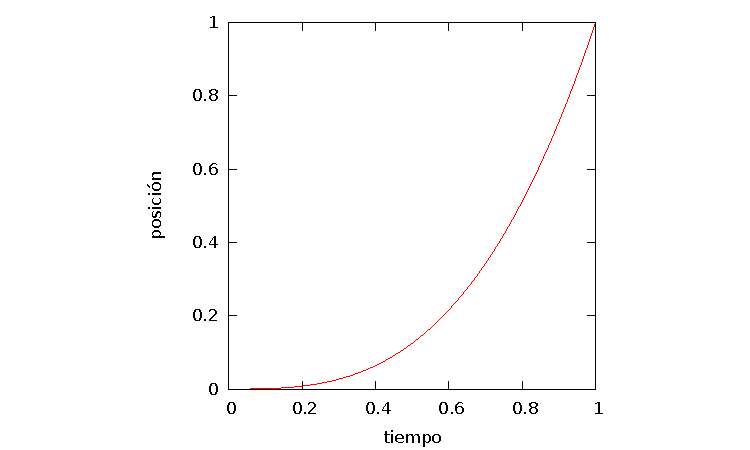
\includegraphics[width=\textwidth]{6_implementacion/imagen_ecuacion1}
  \caption{Relación cúbica entre la posición y el tiempo}
  \label{fig:ecuacion1}
\end{figure}

Tras estudiar bien el código original, se decidió hacer una adaptación en C++,
de forma que se adaptara a las necesidades del proyecto.

\subsection{Adaptación en C++}
El primer paso fue portar las ecuaciones propiamente dichas -- esto es, las
funciones que generaban las posiciones intermedias. Dado que el lenguaje
original, ActionScript, es un derivado de EcmaScript~\cite{Ecmascript}, la
sintaxis es prácticamente idéntica a C++ en cuanto a asignaciones y operadores
se refiere, por lo que este paso fue prácticamente transparente.

Seguidamente, se ideó un \textit{wrapper} para estas ecuaciones, de forma que
fuera un objeto independiente el que se encargara de calcular las posiciones
intermedias de la animación, en lugar de tener que hacerlo los propios objetos
animados. Para ello, se creó la clase \texttt{Animación}, con las siguientes
características:
\begin{itemize}
\item Para cada instancia, permite animar un número arbitrario de valores, de
  forma que con un solo objeto \textit{Animacion} podamos animar la posición
  horizontal y vertical de un objeto, por ejemplo.
\item Permite elegir entre tres tipos de movimiento (\textit{ease in},
  \textit{ease out} y \textit{ease in-out}) para tres ecuaciones distintas
  (cuadrática, cúbica y cuártica), además de una ecuación especial con
  movimiento de ida y vuelta, y, lógicamente, movimiento uniforme. En total, 11
  posibles movimientos.
\item Capacidad para atrasar las animaciones, de forma que sea sencillo generar
  animaciones escalonadas de varios elementos sin tener que recurrir a
  \textit{callbacks}.
\end{itemize}

\subsection{Ejemplo de uso}

Supongamos que tenemos una pelota que queremos mover diagonalmente con un
movimiento de aceleración, desde la posición 0,0 hasta la posición 150, 300, en
30 pasos. Además, tenemos un cuadrado que habrá de moverse de la posición 0, 150
hasta la posición 150,150 cuando la pelota vaya por la mitad de su camino, y que
llegue a la vez que aquella.

Para cumplir este objetivo, crearemos dos objetos \texttt{Animación}, uno para
la pelota y otro para el cuadrado. En el caso de la pelota estaremos animando
dos parámetros, la posición horizontal y la vertical, y la duración será de 30
pasos. El tipo de movimiento será de aceleración, y la ecuación que elegiremos
será la cuadrática. Al no indicarse nada, no habrá espera inicial.

\begin{minted}{cpp}
// Creamos la instancia
Animacion animPelota (2, 30, Animacion::tEaseInQuad, 0);

// Asignamos la pos inicial y final de la coordenada horizontal
animPelota.set(0, 0, 150);  

// Coordenada vertical
animPelota.set(1, 0, 300);
\end{minted}

En el caso del cuadrado el movimiento sólo será horizontal, por lo que
animaremos un parámetro. Además, el movimiento comenzará cuando la anterior
animación vaya por la mitad (esto es, en el paso 15), y deberá llegar a la vez,
por lo que la duración será de 15 pasos.

\begin{minted}{cpp}
// Creamos la instancia de la clase
Animacion animCuadrado (1, 15, Animacion::tEaseInQuad, 15);

// Asignamos las posiciones inicial y final
animCuadrado.set(0, 0, 150);
\end{minted}

Una vez inicializados los objetos \texttt{Animación}, tendremos que hacer que,
en cada iteración del bucle de juego, las animaciones se actualicen. Para ello,
la clase \texttt{Animación} dispone de un método \texttt{update}. Además,
haremos uso del método \texttt{get} para obtener las posiciones intermedias y
así actualizar el objeto

\begin{minted}{cpp}
// ...
// En la fase update del bucle de juego
animPelota.update();
animCuadrado.update();

imagenPelota -> draw(animPelota.get(0), animPelota.get(1));
imagenCuadrado -> draw(animCuadrado.get(0), 150);
\end{minted}

Con esto, ya estará lista la animación de ambos objetos. De cualquier modo, la
clase \texttt{Animación} provee otros métodos que pueden resultar de interés,
como el método \texttt{finished}, que comprueba si las animaciones han
concluído. 

Además, las ecuaciones de los movimientos han sido implementadas en forma de
funciones estáticas, por lo que es posible acceder a las mismas para hacer
cálculos puntuales si fuera necesario. En tal caso, hay que tener en cuenta que
todas las ecuaciones reciben cuatro parámetros, estos son, en orden:

\begin{itemize}
\item Tiempo transcurrido.
\item Valor inicial del atributo a animar.
\item \textit{Delta} del atributo en la animación (final - inicial).
\item Duración de la animación en pasos.
\end{itemize}

Con esto, será posible controlar las animaciones de forma independiente, sin
necesidad de crear una instancia de la clase.


\section{Implementación del analizador básico}
\label{sec:implementacion_analizador}
Como se comentó en la planificación (ver \textit{\nameref{chap:calendario}}), la
viabilidad del proyecto dependía de conseguir una implementación temprana y
correcta del analizador de notas, pues es el núcleo de la aplicación y sin él,
ésta no tendría ningún sentido.

La implementación del analizador se dividió en dos partes. Por un lado, había
que iniciar la captura de audio, lanzando el subsistema de sonido y empezando a
capturar datos. Por otro lado, se tenía que hacer el análisis de los datos
leídos para determinar qué nota se estaba tocando.

\subsection{Lanzando el subsistema de audio}
A lo largo del proyecto se han utilizado distintas bibliotecas de sonido, aunque
en general la filosofía de todas era la misma, así que nos centraremos en los
detalles de la que finalmente se dio por definitiva, PulseAudio. Dentro de
PulseAudio, nos decantamos por la \textit{Simple API}~\cite{pulseaudiosimple},
que cubría todas las necesidades del proyecto sin añadir excesiva complejidad.

El principal concepto en una API de sonido de bajo o medio nivel es el
\textbf{flujo de sonido} o \textit{stream}. Los flujos pueden ser de entrada, de
salida o dúplex, y tienen una serie de características según las necesidades de
la aplicación. En PulseAudio, al tratarse de un servidor de sonido y no de una
simple biblioteca, exiten algunos parámetros necesarios más. Se utiliza la
función \texttt{pa\_simple\_new}, con bastantes parámetros, entre los que se
pueden encontrar:
\begin{description}
\item[Servidor] Normalmente será el servidor de sonido por defecto.
\item[Nombre del cliente y de flujo] Identifica la aplicación (\textit{oFlute})
  y el flujo (\textit{record}) frente al servidor de audio. Este nombre podrá
  verse, por ejemplo, en la aplicación de control de volumen
  (\texttt{pavucontrol}).
  \begin{figure}[ht!]
    \centering
    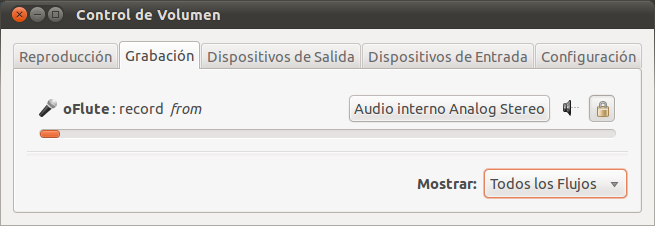
\includegraphics[width=0.7\textwidth]{6_implementacion/imagen_pavucontrol}
    \caption{Control de volumen, mostrando el cliente \textit{oFlute}}
  \end{figure}
\item[Tipo de flujo] En nuestro caso será de entrada, por lo que se utilizó la
  macro \texttt{\nohyphens{kPA\_STREAM\_RECORD}}.
\item[Tipo de \textit{sample}] Definirá el tipo de datos que se usará para
  representar los sonidos.
\item[Opciones de búffering] Según busquemos rendimiento, fiabilidad, poca
  latencia... tendremos que variar las opciones de búffering.
\end{description}

Una vez hayamos creado un flujo, que correrá en segundo plano, tendremos que
leer los datos que arroja. Para ello, la API simple de PulseAudio provee la
función \texttt{pa\_simple\_read}, que nos permitirá volcar en un búffer
temporal un fragmento de audio. La elección del \textbf{tamaño del búffer} es
otro de los valores que repercutirá enormemente en el rendimiento del sistema.

Finalmente, una vez hayamos terminado de leer datos, podremos liberar el flujo
utilizando \texttt{pa\_simple\_free}. Con esto, ya podremos abrir, leer y cerrar
el flujo de sonido del micrófono. 

La parte más compleja a la hora de tratar con flujos es la de elegir los
parámetros apropiados. Son muchísimos los valores que hay que configurar:
frecuencia de muestreo, tamaño del búffer, número de canales, longitud del
búffer intermedio, latencia deseada\ldots Si no sabemos exactamente en qué
influye cada uno, acabamos en un proceso de prueba y error que puede resultar
muy tedioso.

\subsection{Análisis del audio capturado}

La segunda parte del proceso consiste en procesar y analizar el audio capturado
en cada momento, de forma que podamos conocer qué nota se está tocando con la
flauta a través del micrófono.

Como se ha comentado previamente, el alma del procesamiento en este caso es la
aplicación de la \textbf{transformada rápida de Fourier}
(\ref{sec:fourier}). Esta herramienta será capaz de descomponer los fragmentos
de sonido en sus componentes de frecuencia. La biblioteca usada en este caso es
KissFFT~\cite{kissfft}, que da unos resultados muy buenos en cuanto a
rendimiento y precisión. 

En el caso que nos concierne, un procesamiento básico de la señal será
suficiente para poder discernir la nota, por lo que podremos trabajar con
transformadas de fourier reales (no complejas). Para ello, KissFFT ofrece
variantes de sus funciones, muy optimizadas.

El primer paso es inicializar la biblioteca. KissFFT es capaz de utilizar el
mismo búffer entre distintas iteraciones de un cálculo, por lo que ahorramos el
tiempo de guardar y liberar memoria. Esta inicialización se guarda en un objeto
de configuración.

\begin{minted}{cpp}
  kiss_fftr_cfg configFFT = kiss_fftr_alloc (BUFSIZE, 0, NULL, NULL);
\end{minted}

El siguiente paso será realizar el cálculo sobre el búffer de sonido.  La forma
en que el algoritmo FFT almacena sus resultados depende de dos parámetros
principalmente: la frecuencia de muestreo y el tamaño del búffer de entrada. En
el caso de la FFT real, KissFFT devuelve el espectro positivo, que contendrá
tantos valores (en forma de números complejos) como el búffer de entrada más
uno. Cada uno de estos elementos representará la intensidad (y fase) de una
componente de frecuencia en la muestra inicial.

Pero, ¿cómo asociamos cada componente a la frecuencia apropiada? Ahí es donde
entra la frecuencia de muestreo. En el vector que arroja el cálculo del FFT,
haremos una simple regla de tres: el primer elemento corresponderá a la menor
frecuencia (0Hz), y el mayor elemento a la mayor frecuencia audible (en nuestro
caso será 22050Hz, ya que la frecuencia de muestreo es de 44.1kHz, por el
teorema de Nyquist -- sección~\ref{sec:nyquist}).
$$
   \begin{array}{ccc}
       \textrm{Pos. final}  & \longrightarrow & 22050Hz\\
       \textrm{Pos. X} & \longrightarrow & \textrm{Frecuencia Y}
   \end{array}
$$

Una vez identificadas las frecuencias en el resultado de la operación, es
necesario computar la \textbf{magnitud} de cada una de ellas, hallando el módulo
del número complejo. Tras esto, la \textbf{frecuencia fundamental} (que
representará la nota que está tocando la flauta) \textit{debería} ser la que
mayor magnitud tenga.

\subsection{Acotando el resultado}
El siguiente paso fue analizar las frecuencias que proveía la flauta dulce para
las nueve notas que puede emitir utilizando técnicas básicas -- esto es, sin
contar las notas que se pueden emitir utilizando técnicas avanzadas, como tapar
a medias ciertos orificios. De este estudio se extrajeron los siguientes
resultados (tabla \ref{tab:frecuencias}).

\begin{table}[ht!]
  \centering
  \begin{tabular}[h]{|c|c|}
    \hline
    \textbf{Frecuencia aproximada} & \textbf{Nota} \\ \hline
    523.25 Hz & Do, octava 5\\ \hline
    592.163 Hz & Re, octava 5\\ \hline
    656.763 Hz & Mi, octava 5\\ \hline
    699.829 Hz & Fa, octava 5\\ \hline
    785.692 Hz & Sol, octava 5\\ \hline
    893.628 Hz & La, octava 5\\ \hline
    1001.29 Hz & Si, octava 5\\ \hline
    1076.66 Hz & Do, octava 6 \\ \hline
    1195.09 Hz & Re, octava 6 \\ \hline
  \end{tabular}
  \caption{Frecuencias aproximadas de las notas de la flauta dulce}
  \label{tab:frecuencias}
\end{table}

Redondeamos el rango de frecuencias a $[450, 1500]$, cualquier sonido fuera de
ese rango no se considera una nota válida. En el resto de casos, se compara la
frecuencia fundamental obtenida con los valores en la tabla, y se devuelve la
nota apropiada.

\subsection{Ejecución concurrente}

Uno de los problemas que se encontraron fue que, inicialmente, el proceso de
análisis se incluyó dentro de la fase de cálculo de la lógica dentro del
\textit{game loop}. El resultado fue bastante poco satisfactorio, ya que el
cálculo de la FFT ralentizaba mucho el hilo, que tenía que esperar a que
concluyera para seguir renderizando el siguiente fotograma.

Así, se decidió, como suele ser habitual en el desarrollo de videojuegos, mover
el control y análisis del audio a un hilo aparte. Para ello, se hizo uso de la
biblioteca de hilos de Boost, que resulta mucho más amigable y sencilla de usar
que otras alternativas como los \textit{POSIX Threads}. 

A nivel de implementación, el uso de hilos en Boost es muy sencillo. Es
necesario tener una clase con el operador de función -- esto es,
\texttt{operator()} -- sobrecargado. Creamos un objeto de esa clase y se lo
pasamos al constructor de \texttt{boost::thread}, que llamará al anteriormente
citado operador en una copia del objeto pasado.

\begin{minted}{cpp}
// Instancia de la clase
ClaseCallable objeto;

// Hilo, crea una copia de objeto y llama al operador ()
boost::thread hilo(objeto);

// [...]

// Esperamos a que termine el hilo
hilo.join();
\end{minted}

Uno de los problemas que rápidamente se encontraron fue que, al lanzar el hilo,
se hace una copia del objeto referenciado. Esto resultaba un problema, ya que el
analizador hace cierta inicialización previa, y al duplicarse el objeto ocurrían
problemas. El resultado fue utilizar \texttt{boost::ref}, que permite pasar
referencias por copia.

\begin{minted}{cpp}
// Hilo sobre el propio objeto, no se hace copia
boost::thread hilo(boost::ref(objeto));
\end{minted}

\section{Gestión de estados}
\label{sec:implementacion_estados}

La gestión de estados es uno de los retos principales a la hora de desarrollar
un videojuego. Es necesario contar un sistema de gestión de estados robusto, que
permita pasar de un estado a otro de forma sencilla, sin errores, y manteniendo
información entre transiciones si fuera necesario.

En el caso de \textbf{oFlute}, el gestor de estados no necesitaba funciones
avanzadas; las secciones son consecutivas, por lo que no hay necesidad de
incluir concurrencia. Así pues, se editó el gestor de estados en base a la clase
\texttt{Gosu::Window}. Esta clase modela, mediante métodos, las diferentes fases
del \textit{game loop}, a saber:
\begin{enumerate}
\item Gestión de la entrada del usuario, mediante los métodos
  \texttt{buttonDown} y \texttt{buttonUp}.
\item Procesamiento de la lógica, en el método \texttt{update}.
\item Dibujado de los gráficos, en el método \texttt{draw}.
\end{enumerate}

Así, se creó una clase \texttt{Estado} con los mismos métodos, y una clase
\texttt{Juego} (heredera de \texttt{Gosu::Window}), que sirviese de controlador
de estados. Inicialmente, el gestor tenía un método \texttt{cambiarEstado}, que
descargaba de memoria el estado actual y cargaba el siguiente. Durante un tiempo
funcionó bien, pero llegó un momento en que empezaron a aparecer fallos de
memoria difíciles de acotar.

Tras bastantes días de depuración, finalmente el problema se encontró en el
\textit{momento} en el que se hacía la carga y descarga de estados. El conflicto
surgía porque se hacían llamadas para cambiar de estado \textit{en cualquier
  momento}, ya fuera en la etapa de lógica, de dibujado, o de gestión de la
entrada. En el instante de la llamada, se descargaba el estado actual y se
cargaba el siguiente. Esto originaba que las tareas que se habían lanzado, como
por ejemplo las imágenes pendientes de dibujar, se ejecutasen sobre objetos que
habían sido reemplazados en memoria. A menudo las imágenes se encontraban en
búferes de Gosu y no había problema, pero una vez se integró el analizador de
notas, el sistema empezó a fallar.

\label{sec:resolucion_problema_estados}

La solución fue bastante trivial. Se creó un sistema con una pequeña cola de un
elemento en el gestor de estados (la clase \texttt{Juego}). En el momento en que
alguien quisiese cambiar de estado, se añadía a la cola el nuevo estado a
cargar, y se activaba una bandera. Tras completar esa iteración del \textit{game
  loop}, al principio de la siguiente se hacía la carga y descarga de estados.

Este sistema de gestión de estados se extendió para incluir estados concurrentes
(por ejemplo, para mostrar menús de pausa), y aunque no se incluyó en oFlute,
está prevista su integración en la próxima versión de Freegemas~\cite{freegemas}.

\section{Representación de canciones y lecciones}
El sistema de lecciones y el de canciones son los elementos que más dinamicidad
aportan a oFlute. El diseño e implementación de ambos dieron lugar a variadas
cuestiones de diseño. Una de las más importantes fue la forma de representar
lecciones y canciones en el sistema de ficheros.

Desde un principio se decidió que la representación de los ficheros de lecciones
y canciones debería ser sencilla y tener un formato cercano al usuario, para que
se pudiesen crear y modificar mediante el uso de un editor de texto plano.

El primer paso fue descartar por completo el uso de una estructura o notación
propia, ya que dificultaría el proceso de parseo, imposibilitando usar
bibliotecas de terceros para procesar los ficheros de entrada.

El siguiente paso fue comprobar las tecnología de representación más habituales
y utilizadas en el mercado. Se barajaron bastantes posibilidades, y finalmente
redujimos las posibilidades a dos opciones.

\subsubsection{JSON}
JSON (\textit{Javascript Object Notation}~\cite{JSON}) es un formato de
intercambio de datos muy sencillo y liviano, basado en un subconjunto de la
sintaxis de JavaScript. Hoy en día es el formato más utilizado en las
aplicaciones web, ya que el texto que representa la estructura es mínimo.

Se estructura en torno a dos elementos principales:
\begin{description}
\item[Pares] Formados por una clave o nombre, y un valor. Es la forma principal
  de representar un objeto o registro:
  \begin{minted}{javascript}
objeto = { nombre : "Pedro" };    
  \end{minted}
\item[Conjuntos] Que representan arreglos o vectores tradicionales. Lo habitual
  es que formen parte de un \textit{objeto}.
  \begin{minted}{javascript}
objeto = {coordenadas : ["norte", "sur", "este", "oeste"]};
  \end{minted}
\end{description}

Las ventajas de usar JSON son varias. Por un lado, el marcado necesario es
mínimo, por lo que el tamaño de los ficheros es muy reducido. Por otro, la
sintaxis es sencilla y se limita a las dos reglas anteriormente citadas.

\subsubsection{XML}
\label{sec:diseno_xml}
\acs{XML}~\cite{XMLSpec} son las siglas, en inglés, de \textit{eXtensible Markup
  Language} -- lenguaje de marcado extensible, un especificación para la
creación de documentos con marcas definidas por el usuario.

Utiliza una serie de \textit{etiquetas}, organizadas de forma jerárquica, que
siguen la forma \texttt{<nombre>}, donde \textit{nombre} es la identificación
del elemento que se está representando. Las etiquetas deben cerrarse utilizando
la sintaxis \texttt{</nombre>}. Entre las etiquetas de apertura y cierre pueden
anidarse otras etiquetas, así como información en formato texto.

\begin{minted}{xml}
<?xml version="1.0" ?>
<Documento>
  <Nombre>Nombre del documento</Nombre>
  <Autor>Autor del documento</Nombre>
  <Secciones>
    <Seccion>Lorem ipsum dillum</Seccion>
    <Seccion color_texto = "rojo">Sit amet, consectetuer</Seccion>
  </Secciones>
</Documento>  
\end{minted}

XML ofrece varias ventajas, desde el punto de vista de este proyecto, sobre JSON:
\begin{itemize}
\item Aunque la cantidad de texto necesario para marcar un documento es mayor
  que en el caso de JSON, las etiquetas de cierre aportan mayor legibilidad al
  documento, siendo más sencillo saber dónde termina cada bloque.
\item JSON solo permite introducir contenido como propiedades de objetos, usando
  el segundo elemento de los pares \textit{clave/valor}. En XML, es posible
  introducir contenido tanto dentro de las etiquetas como en forma de atributos
  de las mismas, de forma que con un mismo elemento podamos tener varias
  unidades de información.
\item XML es un lenguaje con más tiempo y uso que JSON, y las herramientas y el
  soporte existente es mucho más amplio. La inmensa mayoría de editores ofrecen
  resaltado de sintaxis para esta clase de ficheros, existen herramientas de
  validación XML, etcétera.
\end{itemize}

Por estas y otras razones, finalmente, se acabó eligiendo XML como medio de
representación de las lecciones y las canciones en oFlute.


%%% Local Variables: 
%%% mode: latex
%%% TeX-master: "../memoria"
%%% End: 


\chapter{Pruebas}
Pruebas

\chapter{Conclusiones}
Durante el transcurso del desarrollo de oFlute, y sobre todo al término del
mismo, se han obtenido unas conclusiones y unos resultados, tanto de forma
personal como para con la comunidad, que intentaremos reflejar en este capítulo.

oFlute ha sido el proyecto más longevo al que me he enfrentado hasta ahora. A
pesar de tener conciencia de la envergadura del mismo desde el principio, el
tiempo para completarlo ha superado todas mis expectativas, sobre todo en lo que
a documentación se refiere. La causa de esto ha sido, por un lado, una
planificación inicial algo ineficiente y, por otro lado, mi recelo sobre los
procedimientos actuales sobre ingeniería del software. De cualquier modo, estoy
bastante satisfecho con lo obtenido, y esto me ha servido para aprender a
regirme por una planificación de forma más estricta.

Gracias a oFlute he aprendido las técnicas básicas de la programación de audio,
sobre todo en la parte técnica más que teórica. Es esta parte teórica, sobre
todo la de análisis, la que me gustaría reforzar en un futuro, ahora que cuento
con las bases para conseguirlo. Como se comentó en el capítulo sobre
\textit{Investigación preliminar}, los videojuegos relacionados con el audio son
un nicho aún poco explorado y que puede dar muchas satisfacciones, sobre todo
cuando el producto se orienta a un público joven.

Por otro lado, oFlute también me ha ayudado a aprender a usar algunas
tecnologías secundarias, en algunos casos incluso obteniendo un conocimiento
suficiente para generar documentación e impartir talleres relacionados con ello.

Una de estas tecnologías es \textbf{Boost}~\cite{boost}, un conjunto de
bibliotecas para C++ que amplían en gran medida la biblioteca estándar del
lenguaje. Un amplio número de componentes de Boost formarán parte del nuevo
estándar C++0x~\cite{cpp0x}, por lo que me ha servido para ponerme al día en las
novedades que están por llegar.

Utilizando como material de apoyo el libro \textit{``Beyond the C++ Standard
  Library''}~\cite{libroboost}, pude conocer una gran parte de las bibliotecas
  de Boost, incluyendo punteros inteligentes, programación funcional,
  bibliotecas para hilos, y utilizarlas en el proyecto. Además, también apliqué
  este nuevo conocimiento en el desarrollo de un taller durante los Cursos de
  Verano de la OSLUCA~\cite{cursosverano}, en el que se explicaron las partes más
  importantes de Boost, con numerosos ejemplos de cada una. Toda la
  documentación es libre~\cite{materialesCursoBoost}.

Al tratarse de la principal biblioteca utilizada durante el desarrollo, oFlute
me ha provisto de un profundo conocimiento de \textbf{Gosu}~\cite{gosu},
permitiéndome implementar videojuegos con mucha más fluidez y labrándome un
pequeño \textit{framework} personal que utilizar de base en próximos
proyectos. A raíz de esto impartí un taller~\cite{tallergosu} sobre la
biblioteca en colaboración con la ADVUCA~\cite{advuca}, cuya
afluencia superó las 50 personas. Los materiales pueden descargarse
libremente~\cite{tallergosumateriales}.

Uno de estos proyectos \textit{``hijos''} de oFlute ha sido
\textbf{Freegemas}~\cite{freegemas}, un clon libre del popular juego tipo puzzle
\textit{Bejeweled}. Freegemas es multiplataforma, funciona tanto en GNU/Linux
como en Windows, y además forma parte oficial de Guadalinex~\cite{guadalinex},
por lo que es posible encontrarlo en los repositorios oficiales. 

\begin{figure}[h!]
  \centering
  
\includegraphics[width=0.55\textwidth]{8_conclusiones/imagen_freegemas}
  \caption{Logotipo de Freegemas}
\end{figure}

Además, Freegemas sirvió como base para una serie de tres artículos que
publiqué, junto al doctor Manuel Palomo Duarte, en la revista Linux
Magazine~\cite{linuxmagazine} sobre desarrollo de videojuegos en C++. Es posible
encontrar estos artículos en el archivo de la
revista~\cite{refarticulo1}~\cite{refarticulo2}~\cite{refarticulo3} bajo una
licencia Creative Commons.

Otra de las tecnologías que he aprendido ha sido \textbf{GNU Gettext}, que ha
servido para internacionalizar el proyecto. A este efecto escribí una guía
concisa sobre traducción de proyectos con esta herramienta, que se puede
encontrar en el apéndice~\textit{\nameref{chap:tutorial_gettext}}.

Por otro lado, gracias a oFlute tuve la oportunidad de participar en el IV
Concurso Universitario de Software Libre~\cite{cusl}. En el transcurso del
concurso formé parte de una comunidad muy unida, en la que reinó el apoyo y la
ayuda entre los concursantes. La final del concurso se celebró en la Escuela
Superior de Ingeniería de Cádiz, en la que oFlute obtuvo una mención
especial~\cite{cusl2}.

\begin{figure}[h!]
  \centering
  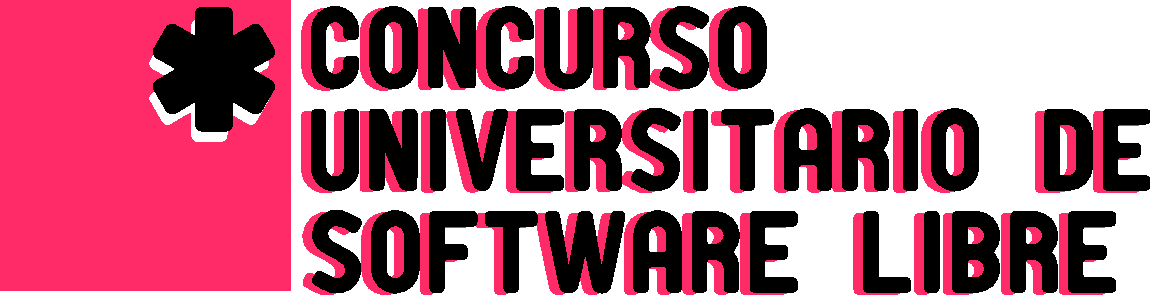
\includegraphics[width=0.65\textwidth]{8_conclusiones/imagen_logocusl}
  \caption{IV Concurso Universitario de Software Libre}
\end{figure}

Previa a la final nacional tuvo lugar la fase local del concurso, en el que el
proyecto también recibió un accésit al mejor proyecto de
innovación~\cite{cusllocal}.

%%% Local Variables: 
%%% mode: latex
%%% TeX-master: "../memoria"
%%% End: 


\appendix

\chapter{Herramientas utilizadas}
En este primer apéndice se hará un repaso por las herramientas que han hecho
posible el desarrollo de oFlute, indicando qué tareas se han llevado a cabo con
cada una de ellas.

Dado que en la actualidad, la tendencia es la de mover la potencia de cálculo a
la \textit{nube}, también se mencionarán las herramientas \textit{online} que
han aportado al proyecto.

\section{Lenguajes y bibliotecas de programación}

\subsection{C++}
El lenguaje elegido para elaborar el proyecto fue \textbf{C++}. C++ es un
lenguaje de programación que extendió el lenguaje original C hacia el paradigma
de la orientación a objetos, mediante el uso de clases, y el paradigma de la
programación genérica, mediante plantillas, además de incluir muchas otras
novedades y facilidades.

Se decidió utilizar C++ por la familiaridad que teníamos con el mismo, así como
por la velocidad y optimización que se obtienen en comparación con otros
lenguajes, como Java.

\subsection{Gosu}
\textbf{Gosu}~\cite{gosu} es una biblioteca libre para el desarrollo de
videojuegos 2D para Ruby y C++. Entre sus características más atractivas se
encuentran la aceleración gráfica por hardware, la sencillez de su API,
completamente orientada a objetos, y su compatibilidad con sistemas GNU/Linux,
Windows y Mac OS.

Esta biblioteca, que está cerca de lanzar su versión 0.8, cuenta con una base de
usuarios cada vez mayor, en parte gracias a su relativa popularidad entre los
desarrolladores indie y en los eventos de programación rápida de videojuegos.

\subsection{PulseAudio}
\textbf{PulseAudio}~\cite{pulseaudio} (mencionado previamente en la sección
\ref{sec:pulseaudio1}) es un servidor de sonido multiplataforma, muy popular en
distribuciones GNU/Linux actuales. Se decidió su uso por lo intuitiva y sencilla
de utilizar que resultaba su API, así como su estabilidad, en comparaciones con
otras opciones previamente probadas.

\subsection{GNU Gettext}

\textbf{GNU Gettext}~\cite{refgettext} es un conjunto de herramientas de internacionalización de
proyectos muy sencilla y popular. Se utilizó porque es la solución más eficaz y
aceptada a la hora de traducir un proyecto. Se puede encontrar un manual
introductorio en el apéndice \textit{\nameref{sec:gettext}}.

\subsection{KissFFT}
\textbf{KissFFT}~\cite{kissfft} es una biblioteca que implementa el algoritmo
FFT para el cálculo de transformadas rápidas de Fourier. Es una biblioteca
pequeña, razonablemente eficiente y portable, con capacidad para realizar
operaciones en distintos formatos.

Dado que el módulo de análisis de sonidos se basa en la transformada de Fourier,
era necesario encontrar una biblioteca que pudiera realizar el cálculo de forma
rápida y precisa. KissFFT resultó ser una candidata ideal para esta tarea.

\subsection{PugiXML}
\textbf{PugiXML}~\cite{pugixml} es una ligera biblioteca para el parseo y
procesamiento de ficheros XML. Tiene soporte completo Unicode, un parseador muy
veloz y capacidad para usar consultas XPath. Además, su implementación apenas
ocupa cuatro ficheros de trivial compilación, por lo que resulta muy sencillo
incluirla en cualquier proyecto.

Esta biblioteca se utilizó para el procesamiento de los ficheros de canciones y
lecciones, que utilizan XML para representar los distintos elementos.

\subsection{Boost}
\textbf{Boost}~\cite{boost} es un conjunto de bibliotecas para C++ para un gran
cantidad de situaciones distintas. Entre sus componentes se incluyen bibliotecas
para el procesamiento de textos, herramientas de gestión de memoria, expresiones
regulares, parseo de opciones de línea de comandos, adaptadores para
programación funcional y un largo etcétera.

Entre sus desarrolladores se encuentran muchos de los mejores programadores de
C++, y tal es su calidad y popularidad, que 10 de las bibliotecas que componen
Boost formarán parte del nuevo estándar de C++.

En oFlute se han utilizado bastantes partes de Boost: punteros inteligentes,
soporte para expresiones regulares, acceso al sistema de ficheros, y operaciones
con cadenas. Esto ha simplificado mucho el código, consiguiendo un estilo más
limpio y elegante, sin sacrificar funcionalidad alguna.

\section{Gestión de código}

\subsection{Subversion}
\textbf{Subversion}~\cite{refsubversion}, popularmente conocido como
\textbf{SVN}, es un sistema de control de versiones muy popular y
utilizado. Hasta hace unos años era el indiscutible ganador entre los sistemas
de control de versiones de código, y en la actualidad sigue siendo la opción
principal en muchas de las forjas de código más importantes de internet.

Se basa en un repositorio central, al que se envían los cambios de
los ficheros versionados. Además, a diferencia de otros sistemas como CVS, lleva
un control de revisiones a nivel global, no a nivel de fichero.

Subversion ha servido, en oFlute, sobre todo como backup online, además de
historial de cambios. En más de una ocasión ha sido necesario revertir los
cambios, y Subversion ha facilitado mucho el proceso, que en otras
circunstancias podría no haber sido posible.

\subsection{Forjas: RedIris y GoogleCode}
Para llevar un control del código del proyecto y servir como punto de encuentro
con otros usuarios y desarrolladores se abrió una forja para oFlute,
inicialmente dentro de la \textbf{Forja de Conocimiento Libre de la Comunidad
  RedIRIS}\footnote{\url{http://forja.rediris.es}}, gestionada por la Junta de
Andalucía. Esta forja ofrecía, además de un sistema de control de versiones del
código, una serie de herramientas para la gestión de bugs, emisión de noticias,
listas de correos, etcétera.

Desafortunadamente la forja de RedIris carecía de un mantenimiento adecuado, lo
que llevó al traspaso del proyecto a \textbf{GoogleCode}~\cite{ofluteforja}, un
repositorio de código ofrecido por Google mucho más actualizado y con un
mantenimiento adecuado. Una de los atractivos de GoogleCode es su sistema de
páginas wiki, que permite gestionar documentación online utilizando una sintaxis
sencilla y potente.

\subsection{Doxygen}
\textbf{Doxygen}~\cite{doxygen} es una herramienta de generación automática de
documentación de código fuente. Basándose en unos comentarios con una sintaxis
especial, Doxygen genera documentación en un gran número de formatos: HTML, PDF,
RTF, \LaTeX...

Esta herramienta se utilizó para generar toda la documentación del código del
proyecto en formato HTML.


\section{Herramientas de diseño y diagramas}

\subsection{Adobe Photoshop}
\textbf{Adobe Photoshop}~\cite{photoshop} es la herramienta de edición gráfica de mapa de bits
más popular y utilizada en el mundo. Su longeva historia y profuso desarrollo ha
hecho que se convierta en la herramienta estándar a la hora de trabajar con
imágenes no vectoriales.

Aunque no se trata de una herramienta libre, se utilizó esta aplicación para la
creación de todo el apartado visual de oFlute. Todas las secciones fueron
diseñadas con esta herramienta, obteniendo un apartado gráfico atractivo y
minimalista.

\subsection{Inkscape}
\textbf{Inkscape}~\cite{inkscape} es una herramienta libre de edición de gráficos vectoriales. A
diferencia de Adobe Photoshop, Inkscape trabaja con formas definidas
matemáticamente, que es posible escalar y distorsionar sin causar pérdida de
datos. Esto hace que sea la herramienta perfecta para trabajar con logotipos y
diagramas.

Esta aplicación ayudó al diseño del logotipo oficial de oFlute, así como al
ajuste de ciertos diagramas pertenecientes a la documentación.

\subsection{Dia}
\textbf{Dia}~\cite{dia} es un editor de diagramas libre, parte de la suite ofimática de
GNOME. Tiene un diseño modular que le permite abordar una gran variedad de
diagramas distintos, desde diagramas de flujo hasta modelos entidad-relación,
UML, etcétera.

Este software se empleó para la generación de la mayor parte de los diagramas
presentes en esta memoria.

\subsection{BoUML}

\textbf{BOUML}~\cite{bouml} es una herramienta libre para diseñar diagramas siguiendo la
notación UML. Cuenta con utilidades de generación automática de código a partir
de diagramas en lenguajes C++, Java, PHP,Python e IDL. Es multiplataforma y
permite la generación de varios tipos de diagramass: diagramas de clases, de
interacción, de secuencia, de casos de uso, etc

\subsection{ImageMagick}

\textbf{ImageMagick}~\cite{imagemagick} es un conjunto de utilidades de línea de comandos para
mostrar, editar y convertir ficheros de imagen. Resultan especialmente útil a la
hora de procesar un gran número de imágenes de forma automática, como por
ejemplo cuando es necesario convertir varias imágenes de un formato a otro, o
cambiar el tamaño de numerosos ficheros.

\section{Edición de textos}

\subsection{GNU Emacs}
\textbf{GNU Emacs}~\cite{refemacs} es un potente editor multiplataforma. Su propio manual lo
describe como \textit{``un editor extensible, personalizable, auto-documentado y
  de tiempo real''}. Emacs es tan potente que a menudo los usuarios
experimentados no tienen que salir de su interfaz para realizar cualquier
operación, ya que desde el propio editor se puede, desde navegar por la red,
hasta revisar el correo electrónico.

Emacs ha sido el editor utilizado para escribir todo el código fuente del
proyecto, así como toda la documentación en \LaTeX. Sus diversos \textit{modos}
se ajustan a cada tipo de documento, proporcionando funciones que faciliten y
aceleren la edición de los textos.

\subsection{\LaTeX}
\textbf{\LaTeX}~\cite{latex} es un sistema de composición de textos, orientado especialmente
a la creación de libros, documentos científicos y técnicos que contengan
fórmulas matemáticas. Es muy utilizado para la composición de artículos
académicos, tesis y libros técnicos, dado que la calidad tipográfica de los
documentos realizados con LaTeX es comparable a la de una editorial científica
de primera línea.

La presente memoria ha sido escrita y maquetada con \LaTeX.


\chapter{Manual de instalación}
\label{sec:maninstalacion}
A continuación se presentan las instrucciones de instalación de \textbf{oFlute}
en sistemas GNU/Linux basados en paquetería Debian \marginpar{Referencia}, por
ser los que más auge están teniendo en la actualidad. Tomaremos como referencia
la distribución Ubuntu 10.04.3 LTS.

\section{Instalación de dependencias}

El primer paso a la hora de instalar oFlute es hacernos con las dependencias del
proyecto. Para ello, utilizaremos el gestor \texttt{apt-get}, pero para otros
sistemas el procedimiento será similar.

La instalación de las dependencias se hará con el siguiente comando:

\marginpar{Desactualizadas}
\begin{minted}{bash}
  sudo apt-get install subversion g++ libgl1-mesa-dev libpango1.0-dev \
libboost1.40-dev libsdl-mixer1.2-dev libsdl-ttf2.0-dev \
libboost-serialization1.40-dev libpulse-dev libboost-regex1.40-dev \
libboost-filesystem-dev libboost-thread-dev 
\end{minted}

Aunque pueda parecer que son numerosas, realmente casi todas las dependencias
forman parte de la instalación de Gosu, la biblioteca de desarrollo de
videojuegos 2D. Al no ser una biblioteca lo suficientemente popular, aún no se
encuentra empaquetada en los repositorios de las principales distribuciones, por
lo que se hace necesario instalarla a partir del código fuente.

\section{Descarga del código fuente}

Seguidamente, hemos de hacernos con una copia local del repositorio, que
contiene el código fuente. Al tratarse de un proyecto libre, el repositorio es
de acceso público\footnote{\url{http://oflute.googlecode.com}}.

Haciendo uso del comando \texttt{svn}, haremos una copia local del repositorio
Subversion \marginpar{Referencia} en nuestro sistema con la siguiente orden:

\begin{minted}{bash}
  svn checkout http://oflute.googlecode.com/svn/trunk oflute
\end{minted}

Con ello, se creará una carpeta llamada \texttt{oflute} en la que se encontrarán
los ficheros de la rama principal (\texttt{trunk}) del proyecto.

\section{Compilación}

Como se ha comentado previamente, será necesario compilar la biblioteca Gosu
previamente. Para ello, se ha facilitado un objetivo en el script de compilación
\marginpar{¿Referencia a algún tutorial de Makefiles?} que automatiza el proceso.

Así, el primer paso será, estando en la carpeta recién creada, utilizar el
siguiente comando:

\begin{minted}{bash}
  make libgosu
\end{minted}

Una vez concluida la compilación de Gosu, pasaremos a compilar el propio
proyecto mediante la siguiente orden:

\begin{minted}{bash}
  make
\end{minted}

\section{Configuración del micrófono}
Antes de poder lanzar el juego, será necesario configurar las opciones de audio
del sistema operativo. Por defecto, la entrada de audio suele estar mutada, por
lo que será imposible que la aplicación tenga acceso al sonido proveniente del
micrófono.

Siguiendo con la referencia de Ubuntu, iremos al menú \textit{Sistema}, luego a
\textit{Preferencias} y, finalmente, elegiremos \textit{Sonido}. Una vez ahí,
pasaremos a la pestaña \textit{Entrada} y, en caso de que estuviera marcada,
desmarcaremos la opción \textit{Silenciar}, tal y como muestra la imagen.

\begin{figure}[h!]
  \centering
  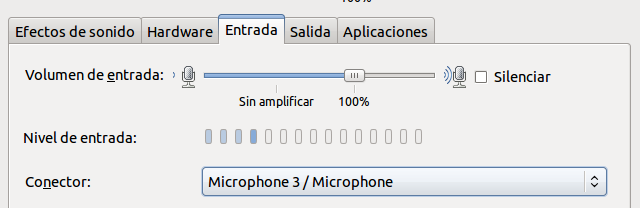
\includegraphics[width=0.9\textwidth]{apendice_manual_instalacion/imagen_captura_1}
  \caption{Panel de configuración del micrófono}
\end{figure}


\section{Ejecución}

Al término de las anteriores etapas, se habrá generado un ejecutable de nombre
\texttt{oflute}, por lo que será posible lanzar la aplicación a través del
siguiente comando:

\begin{minted}{bash}
  ./oflute
\end{minted}



\chapter{Manual de usuario}
\label{chap:manual_usuario}
En este capítulo se explicará el funcionamiento de la aplicación desde el punto
de vista del usuario final, detallando las opciones de cada una de las secciones.

Para poder acceder a la aplicación, tal y como se explicó en el apéndice 
\textit{\nameref{sec:maninstalacion}}, será necesario utilizar el comando:

\begin{minted}{bash}
  ./oflute
\end{minted}

\section{Ejecución inicial}
Al lanzar la aplicación, se abrirá una ventana y aparecerán, consecutivamente,
la pantalla de créditos del autor y la pantalla de presentación del
juego. Pasados unos momentos éstas desaparecerán, aunque tiene la opción de
omitir cada una de las pantallas pulsando la tecla \texttt{escape}.

\begin{figure}[h!]
  \centering
  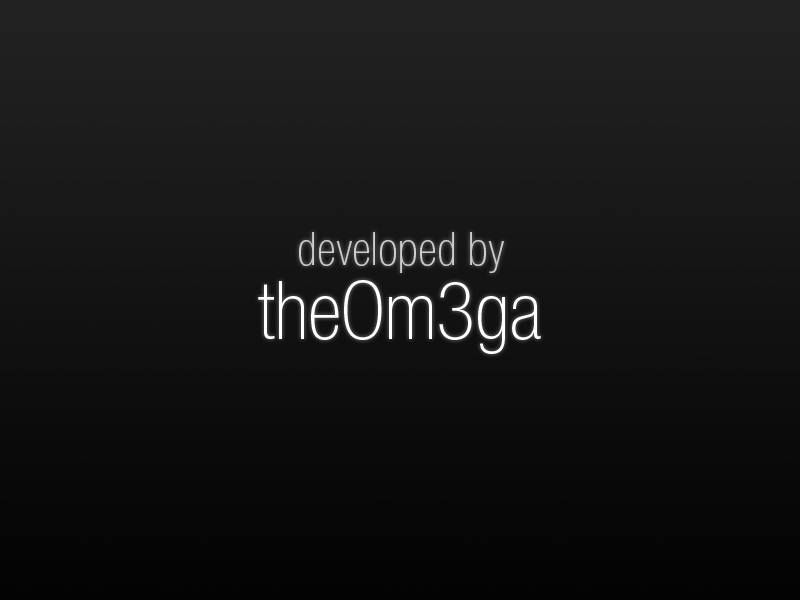
\includegraphics[width=0.8\textwidth]{apendice_manual_usuario/imagen_estadoAutor}
  \caption{Pantalla de créditos del autor}
  \vspace{-1cm}
\end{figure}

\begin{figure}[h!]
  \centering
  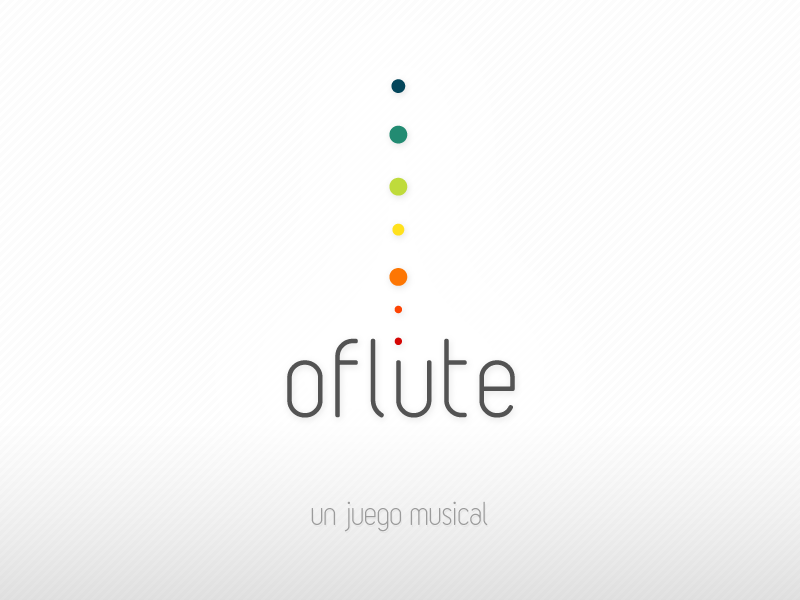
\includegraphics[width=0.8\textwidth]{apendice_manual_usuario/imagen_estadoIntro}
  \caption{Pantalla de presentación del juego}
  \vspace{-0.3cm}
\end{figure}

Una vez desaparezcan ambas pantallas, se iniciará una animación para mostrar el
menú principal. Puede cancelar la animación y mostrar rápidamente el menú
principal pulsando la tecla \texttt{escape}.

\begin{figure}[h!]
  \vspace{-0.1cm}
  \centering
  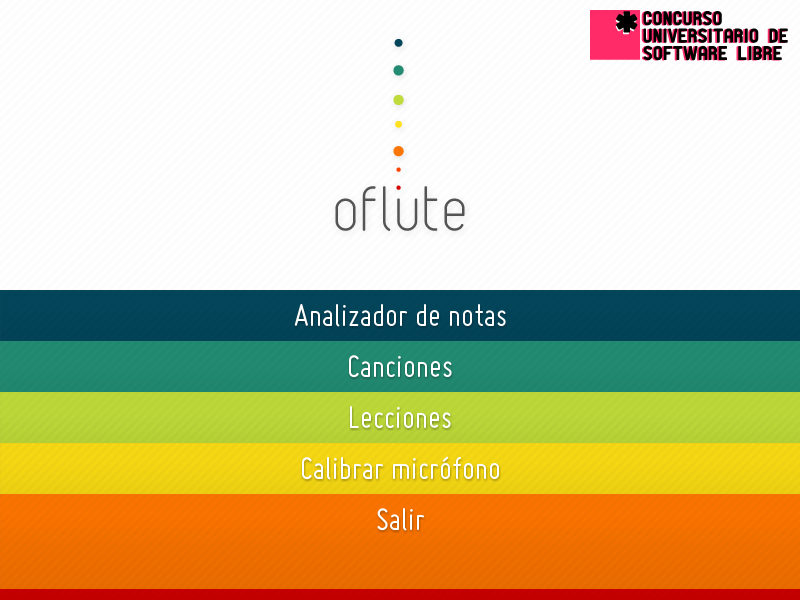
\includegraphics[width=0.8\textwidth]{apendice_manual_usuario/imagen_menuPrincipal}
  \caption{Pantalla del menú principal}
  \vspace{-1cm}
\end{figure}

Cuando las animaciones concluyan, el menú principal ya será completamente
funcional. Podremos acceder a las diferentes opciones, ya sea haciendo click con
el ratón en los botones de pantalla, o pulsando alguna de las teclas de acceso
directo. Las secciones y teclas asignadas son las siguientes:

\begin{itemize}
\item \textbf{Analizador de notas} (\textit{tecla 1}) Abre el analizador de
  notas.
\item \textbf{Canciones} (\textit{tecla 2}) Pasa al menú de selección de
  canciones.
\item \textbf{Lecciones} (\textit{tecla 3}) Abre el menú de elección de
  lecciones.
\item \textbf{Calibrar micrófono} (\textit{tecla 4}) Lanza el sistema de
  calibración del micrófono.
\item \textbf{Salir} (\textit{tecla 5}) Cierra la aplicación
\end{itemize}

Lo recomendado, en la primera ejecución de \textbf{oFlute}, es lanzar la sección
\textit{Calibrar micrófono}, ya sea pulsando el botón con el ratón o mediante la
tecla 4. Con esto nos cercioramos de que el programa es capaz de distinguir el
sonido del micrófono del ruido de fondo. Una vez hecho, ya estará todo listo
para acceder al resto de secciones.

\section{Sección -- calibrar micrófono}
Pulsando el botón correspondiente, o mediante la tecla 4, pasaremos a la sección
de calibración del micrófono. En primer lugar, aparecerá el siguiente mensaje:

\begin{figure}[h!]
  \vspace{-0.1cm}
  \centering
  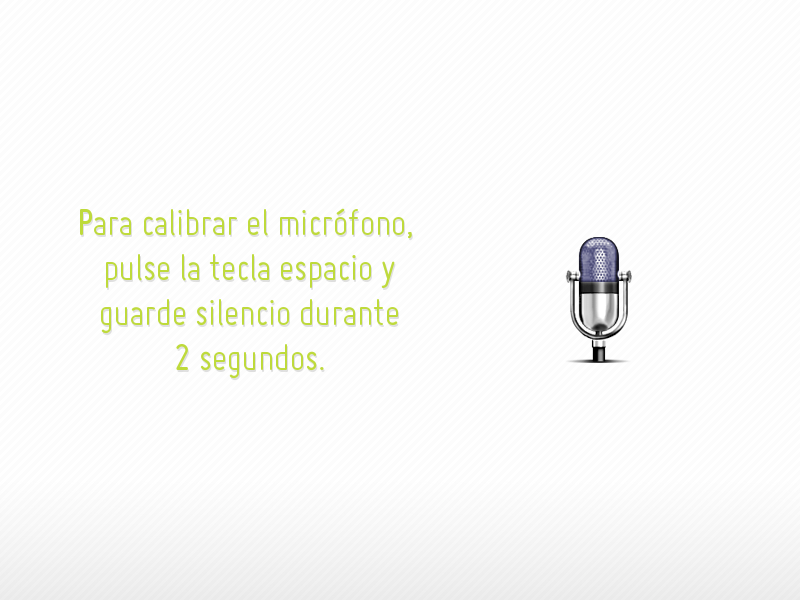
\includegraphics[width=0.8\textwidth]{apendice_manual_usuario/imagen_seccionCalibrar1}
  \caption{Pantalla inicial de calibración del micrófono}
  \vspace{-1cm}
\end{figure}

Como se indica en el mensaje, para comenzar la calilbración el usuario deberá
pulsar la tecla \texttt{espacio} y guardar silencio en el micrófono durante dos
segundos. En ese momento, aparecerá el siguiente mensaje:

\begin{figure}[h!]
  \vspace{-0.1cm}
  \centering
  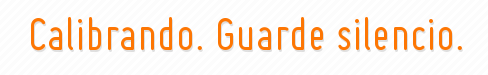
\includegraphics[width=0.8\textwidth]{apendice_manual_usuario/imagen_seccionCalibrar_mensaje1}
  \caption{Mensaje al inicio del calibrado}
\end{figure}

Una vez pasen los dos segundos y concluya la calibración, se mostrará el
siguiente mensaje:

\begin{figure}[h!]
  \vspace{-0.1cm}
  \centering
  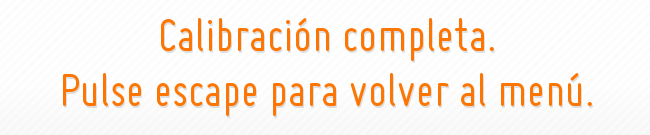
\includegraphics[width=0.8\textwidth]{apendice_manual_usuario/imagen_seccionCalibrar_mensaje2}
  \caption{Mensaje al final del calibrado}
\end{figure}

Cuando concluya el proceso, la aplicación habrá guardado el valor umbral de
ruido del micrófono, lo que facilitará el análisis del sonido de la flauta.

Hay casos en los que la calibración será defectuosa, y un mensaje informará de
ello. En tal caso, no habrá más que comprobar la configuración del micrófono y
repetir el proceso de calibrado.

\section{Sección -- analizador de notas}

Al pulsar el botón correspondiente a la sección del analizador de notas,
mediante una animación aparecerán los elementos de esta parte de la aplicación
(figura \ref{fig:pantalla_analizador_notas} en página
\pageref{fig:pantalla_analizador_notas}).

\begin{figure}[h!]
  \vspace{-0.1cm}
  \centering
  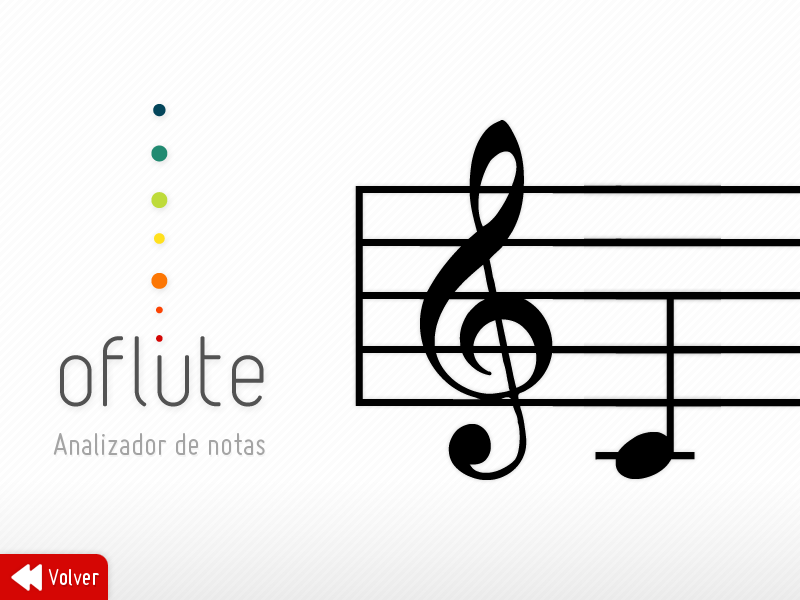
\includegraphics[width=0.75\textwidth]{apendice_manual_usuario/imagen_seccionAnalizador}
  \caption{Pantalla del analizador de notas}
  \label{fig:pantalla_analizador_notas}
\end{figure}

Una vez terminen de mostrarse todos los elementos, el usuario podrá empezar a
utilizar la funcionalidad de la sección. En concreto, el analizador de notas nos
permite ver reflejada en el pentagrama la nota que toquemos con la flauta.

Su uso, pues, es muy sencillo. Simplemente tendremos que tocar nuestra flauta de
forma que el micrófono sea capaz de captar su sonido. Si lo hacemos
correctamente, el analizador mostrará en cada momento la nota que está tocando
sobre el pentagrama.

Una vez hayamos acabado de utilizar esta sección de la aplicación, podremos
pulsar en el botón \textit{Volver}, o en la tecla \texttt{escape} del teclado,
lo que nos llevará de vuelta al menú principal.

\section{Sección -- lecciones}
\vspace{-0.5cm}
Si seleccionamos la opción \textit{Lecciones} en el menú principal, o
alternativamente presionamos la tecla 3 del teclado, la aplicación mostrará una
animación para ocultar el menú principal y nos mostrará el menú de selección de
lecciones. 

\begin{figure}[h!]
  \vspace{-0.2cm}
  \centering
  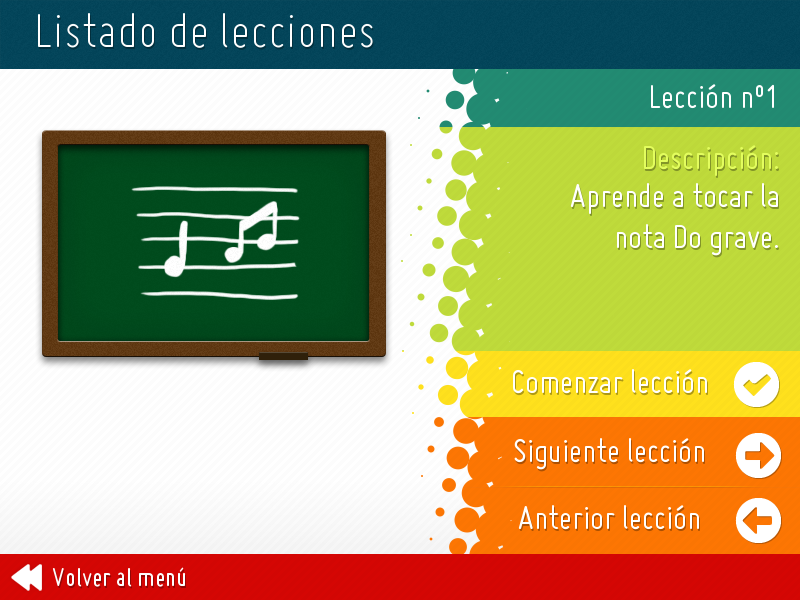
\includegraphics[width=0.75\textwidth]{apendice_manual_usuario/imagen_seccionLecciones1}
  \caption{Pantalla del menú de selección de lecciones}
  \vspace{-1cm}
\end{figure}

\pagebreak

En cualquier momento podemos hacer click en el botón \textit{Volver al menú}, o
pulsar la tecla \texttt{escape} del teclado, para ir a la sección anterior.

En el menú de selección de lecciones podremos encontrar los siguientes
elementos:

\begin{itemize}
\item \textbf{Título} de la lección
\item \textbf{Descripción} de la lección
\item Botón \textbf{Comenzar lección}.
\item Botón \textbf{Anterior lección}.
\item Botón \textbf{Siguiente lección}.
\item Botón \textbf{Volver al menú}.
\end{itemize}

Mediante los botones de \textit{anterior} y \textit{siguiente lección} podremos
navegar entre las diferentes lecciones cargadas en el sistema. Haciendo uso de
los paneles de \textit{título} y \textit{descripción} nos informaremos sobre la
lección elegida. Una vez que tengamos claro la lección que queremos tomar,
pulsaremos en el botón \textit{comenzar lección.}

Una vez que decidamos comenzar la lección, el sistema ocultará los elementos del
menú de selección de lecciones mediante animaciones y, posteriormente, cargará y
mostrará los elementos de la lección elegida.

\begin{figure}[h!]
  \centering
  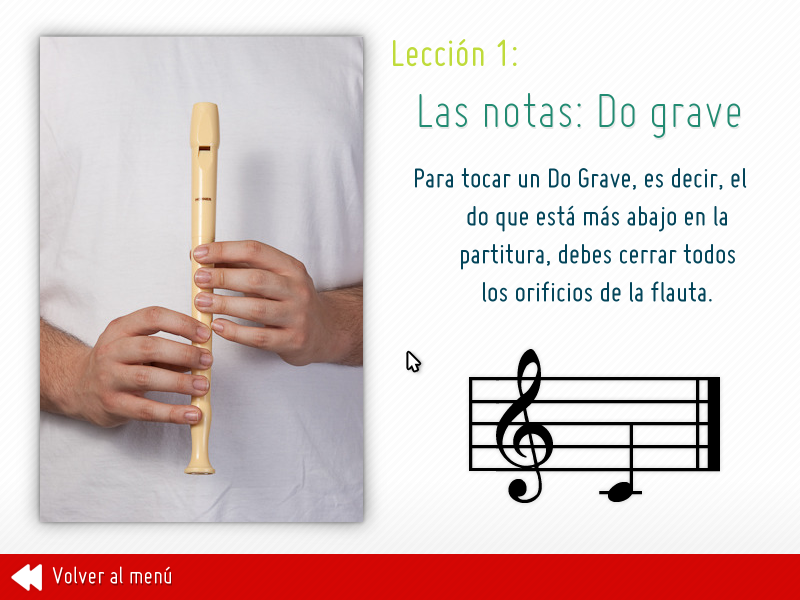
\includegraphics[width=0.8\textwidth]{apendice_manual_usuario/imagen_seccionLecciones2}
  \caption{Pantalla de lección de ejemplo}
\end{figure}

Las lecciones se muestran en forma de conjunto de elementos multimedia --
imágenes y texto -- de fácil comprensión, que el usuario podrá leer y estudiar
de forma independiente. En futuras versiones de la aplicación se podrán utilizar
lecciones de varias etapas, así como integrar sonidos y otro tipo de multimedia.

\section{Sección -- canciones}

El usuario podrá acceder a esta sección desde el menú principal, pulsando en la
botón \textit{Canciones}, o con la tecla 2 del teclado.

Al acceder, desaparecerá el menú principal y se mostrará el menú de selección de
canciones.

\begin{figure}[h!]
  \centering
  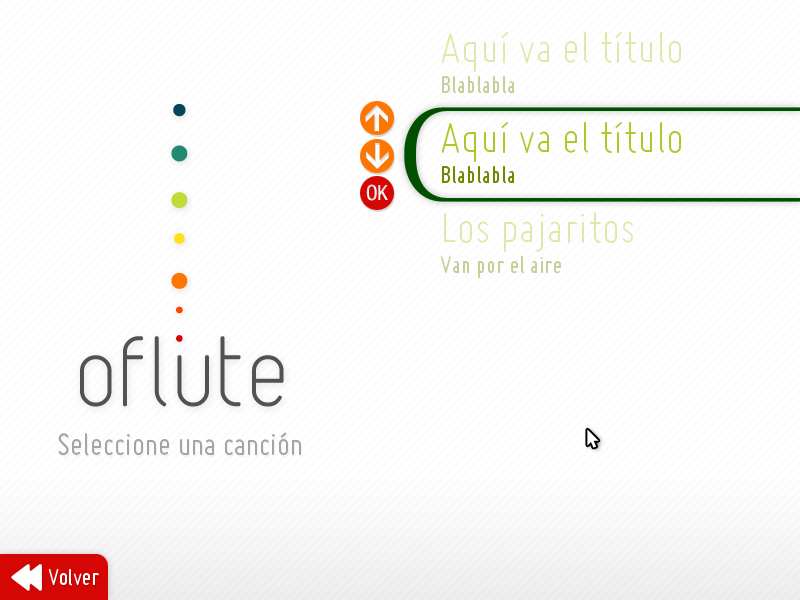
\includegraphics[width=0.8\textwidth]{apendice_manual_usuario/imagen_seccionCanciones1}
  \caption{Pantalla del menú de selección de canciones}
\end{figure}

Esta pantalla consta de los siguientes botones:
\begin{itemize}
\item \textbf{Anterior canción}, representado con una flecha hacia arriba.
\item \textbf{Siguiente canción}, representado con una flecha hacia abajo.
\item \textbf{Comenzar canción}, simbolizado con la palabra \textit{OK}.
\item \textbf{Volver}.
\end{itemize}

Mediante los botones \textit{anterior} y \textit{siguiente canción}, el usuario
podrá elegir el tema a interpretar con la flauta. Una vez esté resaltada la
canción correcta, el usuario deberá pulsar el botón \textit{Comenzar canción --
  OK} para que dé comienzo la interpretación.

También es posible pulsar el botón \textit{volver} para ir de nuevo al menú
principal.

\subsection{Interpretación de la canción}

Al lanzar la canción, aparecerá la pantalla de interpretación de canción, que
contiene numerosos elementos importantes para el jugador.

\begin{figure}[h!]
  \centering
  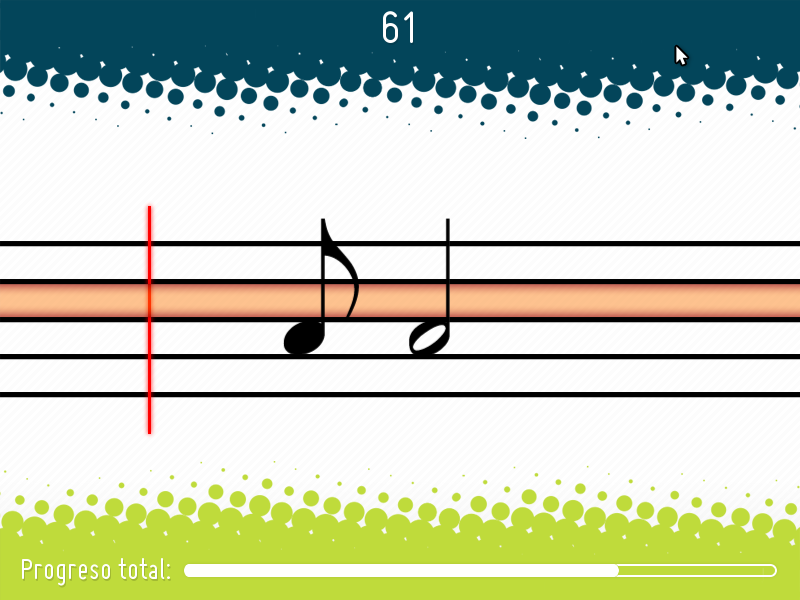
\includegraphics[width=0.8\textwidth]{apendice_manual_usuario/imagen_seccionCanciones2}
  \caption{Pantalla de interpretación de canción}
\end{figure}

\begin{enumerate}
\item \textbf{Marcador} de la puntuación del usuario.
\item \textbf{Pentagrama}. Sobre él aparecerán las notas.
\item \textbf{Notas}. Éstas irán apareciendo por el lado derecho del pentagrama,
  y moviéndose hacia la izquierda de forma ordenada y rítmica.
\item \textbf{Resaltado de nota}. Resalta la posición en el pentagrama de la
  nota que está tocando el usuario con la flauta en cada momento. Esto ayuda
  visualmente a saber si estamos interpretando la nota correcta o no.
\item \textbf{Barra de interpretación}. Esta barra indica cuándo debe el usuario
  empezar a tocar la nota. 
\item \textbf{Barra de progreso}. Indica el progreso de la interpretación de la
  canción. Cuando la barra esté completa, la canción concluirá.
\end{enumerate}

La forma de juego es sencilla. Como se ha indicado, las notas aparecerán sobre
el pentagrama por el lado derecho, e irán desplazándose hacia la izquierda. Una
vez que una nota llegue a la \textit{barra de interpretación}, el jugador deberá
tocar con la flauta la nota correcta, de forma constante hasta que llegue el
turno de la siguiente nota.

Para ayudar al jugador, la barra de \textit{resaltado de nota} indicará en cada
momento qué nota se está tocandoo. Así, si en un instante es necesario tocar un
\textit{Sol} pero la barra de resaltado está por encima, el usuario sabrá que
debe cerrar más orificios de la flauta.

Las posibles \textbf{notas} que pueden aparecer son \textit{Do}, \textit{Re},
\textit{Mi}, \textit{Fa}, \textit{Sol}, \textit{La}, \textit{Si}, \textit{Do
  grave} y \textit{Re grave}. Las posibles figuras que podrán aparecer son las
siguientes:

\begin{description}
\item[Redonda] -- Dura cuatro tiempos.
\vspace{-0.1cm}
\begin{figure}[h!]
  \centering
  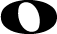
\includegraphics[width=0.05\textwidth]{apendice_manual_usuario/imagen_figRedonda}
  \caption{Figura musical -- Redonda}
\end{figure}

\vspace{-0.35cm}

\item[Blanca] -- Dura dos tiempos.
\vspace{-0.1cm}
\begin{figure}[h!]
  \centering
  \subfloat[Posición normal]{\parbox{0.5\textwidth}{\centering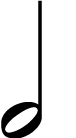
\includegraphics[width=1cm]{apendice_manual_usuario/imagen_figBlanca}}}
  \subfloat[Posición invertida]{\parbox{0.5\textwidth}{\centering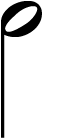
\includegraphics[width=1cm]{apendice_manual_usuario/imagen_figBlancaInv}}}
  \caption{Figura musical -- Blanca}
\end{figure}

\vspace{-0.35cm}

\item[Negra] -- Dura un tiempo.
\vspace{-0.1cm}
\begin{figure}[h!]
  \centering
  \subfloat[Posición normal]{\parbox{0.5\textwidth}{\centering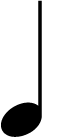
\includegraphics[width=1cm]{apendice_manual_usuario/imagen_figNegra}}}
  \subfloat[Posición invertida]{\parbox{0.5\textwidth}{\centering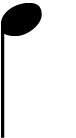
\includegraphics[width=1cm]{apendice_manual_usuario/imagen_figNegraInv}}}
  \caption{Figura musical -- Negra}
\end{figure}

\vspace{-0.35cm}

\item[Corchea] -- Dura la mitad que una negra.
\vspace{-0.1cm}
\begin{figure}[h!]
  \centering
  \subfloat[Posición normal]{\parbox{0.5\textwidth}{\centering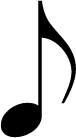
\includegraphics[width=1cm]{apendice_manual_usuario/imagen_figCorchea}}}
  \subfloat[Posición invertida]{\parbox{0.5\textwidth}{\centering\includegraphics[width=1cm]{apendice_manual_usuario/imagen_figCorcheaInv}}}
  \caption{Figura musical -- Corchea}
\end{figure}
\end{description}

\vspace{-0.35cm}

De manera excepcional, es posible alargar el tiempo de una figura mediante el
uso del \textbf{puntillo}, que hará que su duración aumente la mitad de su
tiempo original. El puntillo se representa mediante un pequeño círculo a la
derecha de la base de la nota.

Por otro lado, las siguientes son las figuras que representan los silencios


\chapter{Manual para añadir nuevas canciones}
\label{chap:manual_canciones}
En \textbf{oFlute} existe la posibilidad de añadir nuevas canciones al juego, de
forma que los usuarios puedan ampliar el juego y que éste se convierta en una
herramienta lúdica prácticamente ilímitada.

Así, en un futuro podrán existir, por ejemplo, packs temáticos de canciones
descargables desde internet, con los que seguir practicando nuestra pericia con
la flauta dulce.

\section{Ficheros necesarios}

Cada una de las canciones presentes en el juego necesitará un fichero donde se
definirán las características y notas de la canción. El nombre de estos ficheros
sigue la estructura \texttt{songN.xml}, donde \textit{N} es el número de canción
a añadir.

Los ficheros de las canciones se encuentran en la carpeta \texttt{canciones},
ubicada en el directorio raíz de la instalación de oFlute. 

\section{Estructura del fichero de canciones}

\subsection{Lenguaje XML}

Cada fichero de canción es un archivo \textit{XML}. \marginpar{REFERENCIA} XML
son las siglas, en inglés, de \textit{eXtensible Markup Language} -- lenguaje de
marcado extensible. La tecnología XML busca dar solución al problema de expresar
información estructurada de la manera más abstracta y reutilizable posible. 

Para ello, utiliza una serie de \textit{etiquetas}, organizadas de forma
jerárquica, que siguen la forma \texttt{<nombre>}, donde \textit{nombre} es la
identificación del elemento que se está representando. Las etiquetas deben
cerrarse utilizando la sintaxis \texttt{</nombre>}. Entre las etiquetas de
apertura y cierre pueden anidarse otras etiquetas, así como información en
formato texto.

Todo documento XML tiene una etiqueta \textit{raíz}, de la cual cuelgan todas
las demás. En nuestro caso, los ficheros que representan las canciones tendrán
como raíz el elemento \texttt{Song}. Este es un ejemplo de un fichero completo:



\begin{minted}{xml}
<?xml version="1.0" ?>
<Song>
  <Title>Los pajaritos</Title>
  <Desc>Van por el aire</Desc>
  <BPM>60</BPM>
  <Notes>do5n mi5c fa5c sol5n sol5c sol5c la5n la5c la5c sol5n 
   sol5n fa5n fa5n mi5n mi5n re5c mi5c fa5c re5c do5n do5n</Notes>
</Song>
\end{minted}

\subsection{Campos iniciales}

\subsubsection{Título de la canción}

%\usestyle{default}

El título de la canción se indicará mediante la etiqueta \texttt{<Title>}, por ejemplo:

\inputminted{xml}{apendice_manual_canciones/snippet_1}


\chapter{Manual para añadir nuevas lecciones}
\textbf{oFlute} fue diseñado de forma que se pudiera expandir de manera
sencilla. Además de poder añadir canciones nuevas tal y como se explicó en el
apéndice \textit{\nameref{chap:manual_canciones}}, también es posible añadir
nuevas lecciones a la aplicación.

\section{Ficheros necesarios}

Las lecciones necesitan de más ficheros que las canciones, ya que se basan en
elementos multimedia para mejorar la experiencia de usuario. Así, una lección
dispondrá de un fichero base en formato XML y de una serie de archivos
auxiliares de recursos. Por ahora, \textbf{oFlute} acepta recursos en formato
imagen PNG \marginpar{REFERENCIA} y fuentes TTF, pero en un futuro será posible
añadir otros tipos de elementos.

\subsection{Fichero de lección}
El fichero base deberá alojarse en el directorio \texttt{lecciones}, dentro de
la carpeta raíz de la instalación de oFlute. Además, su nombre debe seguir la
estructura \texttt{lecN.xml}, donde \textit{N} es el número de la lección a
añadir.

\subsection{Ficheros de recursos}
Los ficheros de recursos podrán guardarse en cualquier lugar dentro de la
carpeta de instalación de oFlute. De cualquier modo, se recomienda guardar las
imágenes en la carpeta \texttt{media/lecciones} y las fuentes en la carpeta
\texttt{media}, ya que es ahí donde están los recursos de las otras lecciones,
facilitando la reutilización.

\section{Estructura del fichero de lección}

Como se comentó en la sección \ref{sec:lenguaje-xml}, todos los documentos XML
necesitan un elemento raíz. En este caso, usaremos la etiqueta \texttt{<Lec>}
como raíz del fichero de lección.


\subsection{Campos iniciales}

\subsubsection{Índice}
Es posible añadir el índice de la lección, de forma que podamos decidir
fácilmente el orden en que aparecerá dentro de la lista de lecciones del sistema.

Para ello, utilizaremos la etiqueta \texttt{<index>}, tal que así:

\inputminted{xml}{apendice_manual_lecciones/snippet_1}

\subsubsection{Nombre}
El nombre de la lección lo añadiremos utilizando la etiqueta
\texttt{<nombre>}. Éste se utilizará en la pantalla de selección de lecciones.

\inputminted{xml}{apendice_manual_lecciones/snippet_2}

\subsubsection{Descripción}

La descripción de la lección nos permitirá conocer brevemente su contenido sin
tener que acceder directamente a la misma. Se empleará la etiqueta
\texttt{<descrip>} para identificar la descripción.

\inputminted{xml}{apendice_manual_lecciones/snippet_3}

\subsection{Elementos multimedia}
Tras los campos iniciales, se indicarán los elementos multimedia. Podremos
encontrar dos tipos: imágenes, cargadas a partir de los ficheros de recursos
previamente comentados, y textos, que se dibujan de forma dinámica. Para ello,
marcaremos una sección con la etiqueta \texttt{<elementos>}.

\begin{minted}{xml}
<elementos>
...
</elementos>  
\end{minted}

Cabe notar que todos los elementos multimedia aparecerán en pantalla mediante
una animación de desvanecimiento o \textit{fade-in}. Para indicar el orden en
que éstos aparecerán, las etiquetas de los elementos multimedia tendrán un
atributo \texttt{wait}, que indica el retraso en el inicio de la animación.

\subsubsection{Imágenes}
Las imágenes se indicarán mediante la etiqueta simple \texttt{<img/>} --
\textit{simple}, porque se cerrará a sí misma, desapareciendo la etiqueta de
cierre posterior.

Esta etiqueta tendrá los siguientes atributos:
\begin{description}
\item[src] Indica la ruta al fichero de imagen, relativa al directorio raíz de
  oFlute.
\item[x, y, z] Posición horizontal, vertical y profundidad del elemento en
  pantalla, en píxeles.
\item[wait] Como se ha comentado, es el retraso en la animación de aparición.
\end{description}

Un ejemplo de definición de elemento multimedia en formato imagen podría ser el
siguiente:

\inputminted{xml}{apendice_manual_lecciones/snippet_4}

\subsubsection{Textos}
Los textos utilizan la etiqueta \texttt{<texto>}. Dentro de la etiqueta, esto
es, entre la etiqueta de apertura \texttt{<texto>} y la de cierre
\texttt{</texto>}, se habrá de escribir el texto que queremos que se
muestre. Hay que tener en cuenta que los saltos de línea que insertemos
aparecerán tal cual posteriormente en pantalla.

Además, la etiqueta consta con numerosos atributos obligatorios:
\begin{description}
\item[tam] Indica el tamaño de la fuente en pantalla.
\item[ca, cr, cg, cb] Para definir el color del texto utilizamos su definición
  RGBA (\textit{Red, Green, Blue, Alpha})\marginpar{REFERENCIA}, esto es, los
  valores individuales de los canales rojo, verde, azul y alfa (opacidad). Así,
  cada uno de los atributos indica el valor de un canal:
  \begin{description}
  \item[ca] Canal alfa.
  \item[cr] Canal rojo.
  \item[cg] Canal verde.
  \item[cb] Canal azul.
  \end{description}
\item[x, y, z] Definen la posición horizontal, vertical y profundidad del texto
  en pantalla.
\item[align] Indica la alineación del bloque de texto. Valdrá 1 para alineación
  a la izquierda, 2 para alineación centrada y 3 para alineación a la derecha.
\item[sombra] Indica si el texto tendrá sombra o no, con un valor 0 ó 1. En el
  caso de que valga 1, habrá que indicar un atributo adicional,
  \textbf{opacSombra}, que indicará la opacidad de la sombra.
\item[wait] Retraso en la animación de aparición.
\end{description}

Como ejemplo de bloque de texto, podemos poner el siguiente fragmento:

\inputminted{xml}{apendice_manual_lecciones/snippet_5}


\chapter{Manual de traducción de proyectos con GNU Gettext}
\label{sec:gettext}
%\lstset{style=C++}

%\setlength{\parskip}{0.3cm plus 3mm}
\setlength{\parindent}{0.3cm}
\section{Antecedentes}
Durante el desarrolllo del proyecto surgió la necesidad de preparar el proyecto
para su traducción. Inicialmente se optó por utilizar un sistema propio de
traducción, basado en un script en Python y en una pequeña clase que generaba un
diccionario según el idioma elegido. Sin embargo, esta opción resultó
ineficiente y, sobre todo, alejada del resto de soluciones estándar a la hora de
traducción de proyectos. 

Por ello, se decidió investigar sobre las tecnologías de traducción más
utilizadas en el panorama del software libre, y finalmente se optó por \textbf{GNU
Gettext}~\cite{refgettext}. Para afianzar los conocimientos y facilitar el aprendizaje a 
otros desarrolladores, se editó el presente documento.

La primera edición del manual se presentó en el I
Hackathón~\cite{refhackathonUCA} organizado por la Oficina de Software Libre y
Conocimiento Abierto de la Universidad de Cádiz, acompañada de un pequeño taller
con una demostración en vivo. Se encuentra disponible para su descarga en el
repositorio Rodin de la UCA~\cite{refmanualgettext} y se puede difundir
bajo los términos de la licencia \textit{Creative Commons - Reconocimiento,
  Compartir igual 3.0}~\cite{commonsbysa}

\section{Introducción}

\textbf{GNU Gettext} es un conjunto de herramientas libres de
internacionalización que permite traducir nuestros proyectos de una manera
sencilla. Es el sistema de i18n\footnote{\textit{``i18n''} es una alternativa a
  escribir \textit{internacionalización}, el 18 simboliza los 18 caracteres
  entre la \textit{i} inicial y la \textit{n} final} más utilizado, pudiendo
encontrarse en una gran cantidad de proyectos.

Las ventajas de usar un sistema como \textit{Gettext} en lugar del
típico menú de elección de idiomas dentro de la aplicación son
muchas. Por ejemplo, con Gettext el ajuste del idioma es transparente
al usuario. Además, ofrece todas las ventajas de usar un sistema
establecido y prácticamente estándar.

\subsection{Internacionalización vs localización}

La \textit{internacionalización} de un proyecto consiste en prepararlo de forma
que sea capaz de trabajar y presentarse en una multitud de idiomas y
configuraciones regionales. Por otro lado, la \textit{localización} trata de
coger un programa internacionalizado y darle la suficiente información para que
se adapte al idioma y configuración del usuario actual.

\subsection{El paquete de herramientas de GNU Gettext}

GNU Gettext está compuesto de un conjunto de elementos que forman un
\textit{framework} de trabajo común. En particular, esto incluye:
\begin{itemize}
\item Una serie de directivas y convenciones a la hora de escribir el código
  fuente de nuestro proyecto.
\item Un esquema estándar de organización de ficheros y directorios para guardar
  los ficheros relacionados con la traducción.
\item Una biblioteca que provee funciones relacionadas con las cadenas
  traducidas.
\item Algunas utilidades para la creación y edición de los ficheros con las
  cadenas de traducción.
\item Un modo de edición para \textbf{Emacs}.
\end{itemize}

\section{Pasos en el proceso de traducción}

A la hora de adaptar un proyecto para internacionalizarlo hay que seguir una
serie de pasos bastante mecánicos que se repiten cada vez que añadamos o
modifiquemos las cadenas de nuestro proyecto.

\subsection{Adaptación del código fuente}

Primero, necesitamos adaptar el código de nuestro programa, marcando de alguna
forma las cadenas que queremos que queden traducidas. Podría pensarse que este
paso podría ser automático, pero hay cadenas que a buen seguro no queremos que
sean traducidas, como por ejemplo parámetros de funciones o mensajes con campos
variables, como los que se utilizan con la función \texttt{printf}.

Para ello, añadiremos las siguientes líneas al inicio de nuestro fichero fuente:
\begin{minted}{cpp}
#include <libintl.h>
#include <locale.h>
#define _(x) gettext(x)
\end{minted}

La biblioteca \texttt{libintl} será la encargada de la internacionalización de
nuestro proyecto, siendo de especial interés su función \texttt{char *
  \textbf{gettext} (const char *)}, a la que le pasaremos las cadenas originales
y nos devolverá la cadena traducida dependiendo del \textit{locale} del
sistema. Para hacer menos evidente su uso, utilizamos la macro definida arriba.

\begin{nota} Habitualmente, es una buena práctica en el desarrollo de un
  proyecto libre el usar el inglés como idioma por defecto para los mensajes de
  interacción con el usuario. Gettext supone que se usará el inglés como
  lenguaje principal, por lo que nos acogerémos a esta práctica.
\end{nota}

El siguiente paso será cambiar todas las cadenas que queramos traducir en
nuestro proyecto, de forma que en realidad sean siempre llamadas a la función
\texttt{gettext}, o preferiblemente a su macro \texttt{\_()}.
\begin{minted}{cpp}
  string mensaje = "Hello world";
\end{minted}
Pasará a ser:
\begin{minted}{cpp}
  string mensaje = _("Hello world");
\end{minted}

\medskip

Algo a tener en cuenta es que es necesario elegir un nombre para el
\textit{dominio} de la internacionalización, que por regla general coincidirá
con el proyecto. En nuestro ejemplo, este nombre será \textbf{oflute}.

\medskip

En las primeras líneas de nuestro proyecto añadiremos las siguientes
instrucciones de inicialización:

\begin{minted}{cpp}
bind_textdomain_codeset ("oflute", "UTF-8");
setlocale(LC_ALL, "");
bindtextdomain("oflute", "lang" );
textdomain("oflute");
\end{minted}

Eso le indicará a la biblioteca de i18n cuál es el dominio de la
traducción, así como el directorio de las traducciones
(\texttt{lang}), y pondrá el locale por defecto.

\medskip

Así pues, un posible fichero \texttt{main.cpp }de ejemplo podría ser:

\begin{minted}{cpp}
#include <iostream>
#include <libintl.h>
#include <locale.h>

#define _(x) gettext(x)

using namespace std;

int main(int argc, char *argv[])
{
    bind_textdomain_codeset ("oflute", "UTF-8");
    setlocale(LC_ALL, "");
    bindtextdomain("oflute", "lang" );
    textdomain("oflute");

    cout << _("Hello world") << endl;
    return 0;
}

\end{minted}

\subsection{Generando los ficheros de traducción}

Una vez que tengamos todas las cadenas a traducir apropiadamente
adaptadas como se ha comentado antes, pasaremos a crear los ficheros
con los que realizaremos las traducciones. Hay varios tipos de estos
ficheros:

\begin{description}
\item[.POT] \textit{(Portable Object Template)} Es el primer fichero
  que se genera, y contiene todas las cadenas extraídas del código
  fuente, que servirá luego como plantilla para los ficheros
  \texttt{.po}.

\item[.PO] \textit{(Portable Object)} Son los ficheros principales de
  traducción, los que se editan con las cadenas traducidas. Hay uno
  por cada \textit{locale} que queramos incluir.

\item[.MO] \textit{(Machine Object)} Son la versión binaria de los
  ficheros \texttt{.po}, los que nuestra aplicación usará para leer
  las cadenas traducidas.
\end{description}

\medskip

La forma de organizar los diferentes ficheros está bastante
estandarizada, de forma que lo más recomendado es seguirla -- de no
hacerlo podemos tener problemas a la hora de que el programa encuentre
los ficheros de traducción.

\begin{itemize}
\item En la raíz de nuestro proyecto tendremos una carpeta \textbf{po}
  que albergará el fichero de plantilla \texttt{.pot}, en nuestro caso
  \texttt{oflute.pot}, así como los ficheros \texttt{.po} de cada
  \textit{locale}: \texttt{en.po}, \texttt{es.po}, etc.
\item Además, también en la raíz tendremos otra carpeta llamada
  \textbf{lang}. Dentro de ella habrá una carpeta por cada fichero
  \texttt{.po} en la carpeta antes mencionada, y dentro de cada una de
  ellas, una carpeta \texttt{LC\_MESSAGES}, que albergará el fichero
  \texttt{.mo} correspondiente, todos con el nombre del dominio, en
  nuestro caso \texttt{oflute.mo}
\end{itemize}

La estructura de directorios que obtendremos será algo así:

\begin{verbatim}
lang
|-- en
|   `-- LC_MESSAGES
|       `-- oflute.mo
`-- es
    `-- LC_MESSAGES
        `-- oflute.mo
po
|-- en.po
|-- es.po
`-- oflute.pot

\end{verbatim}

\subsubsection{Creando la plantilla .pot}

Así pues, el primer paso será generar el fichero \texttt{.pot}. Para ello
utilizaremos la utilidad \texttt{xgettext}. Así pues, creamos los directorios
antes comentados y usamos la siguiente expresión:

\begin{minted}{bash}
xgettext \
   --package-name oflute \
   --package-version 0.1 \
   --default-domain oflute \
   --output po/oflute.pot \
   --from-code=utf-8 \
   --copyright-holder="Tu nombre" \
   --msgid-bugs-address="tu@mail.com" \
   -s -k_ -C main.cpp
\end{minted}

La mayoría de las opciones son autoexplicativas, pero es interesante
conocer el significado de las que no lo son:

\begin{description}
\item[-s] Salida ordenada, ordena las cadenas en el fichero de
  plantilla, útil cuando tenemos muchos ficheros fuente y queremos
  tener las cadenas organizadas.
\item[-k\_] Indica que también busque cadenas marcadas con
  \texttt{\_(cadena)} además de \texttt{gettext(cadena)}.
\item[-C] Indica que el lenguaje es C++.
\end{description}

Con esto tendremos el fichero en \texttt{po/oflute.pot}. Es necesario editarlo y
cambiar el valor de \texttt{CHARSET} (en la línea \texttt{Content-Type: ...})
por \texttt{UTF-8}, \texttt{xgettext} aún no ofrece ninguna opción para
autorrellenar este campo.

\subsubsection{Creando los ficheros de traducción .po}

El siguiente paso será el de crear un fichero \texttt{.po} para cada uno de los
idiomas a los que queramos traducir nuestro proyecto. Para ello utilizaremos la
utilidad \texttt{msginit} de la siguiente manera, suponiendo los idiomas inglés
y español:

\begin{minted}{bash}
msginit -l es -o po/es.po -i po/oflute.pot
msginit -l en -o po/en.po -i po/oflute.pot
\end{minted}

Al ejecutar los comandos nos pedirán nuestro email, de forma que sea posible
recibir feedback sobre la traducción que hagamos.

\medskip

Si le echamos un vistazo al fichero \texttt{po/es.po}, después de todas las
cabeceras iniciales, nos encontraremos con las cadenas de nuestro programa de la
siguiente manera:

\begin{minted}{po}
#: main.cpp:15
msgid "Hello world"
msgstr ""
\end{minted}

El formato es muy sencillo: la primera línea indica la situación de la
cadena en el código fuente, la segunda es la cadena original, y la
tercera es la cadena traducida. Para el fichero en español, quedaría:

\begin{minted}{po}
#: main.cpp:15
msgid "Hello world"
msgstr "Hola mundo"
\end{minted}

Cabe notar que, como el lenguaje original es el inglés, podemos dejar el fichero
\texttt{en.po} intacto, ya que por defecto utilizará las cadenas originales.

\subsubsection{Creando los binarios .mo}

Una vez terminado el apartado anterior, nos queda el último paso, que es generar
los ficheros binarios con las traducciones. Para ello, utilizaremos la utilidad
\texttt{msgfmt}, que convertirá los \texttt{.po} en \texttt{.mo}, de la
siguiente manera:

\begin{minted}{bash}
mkdir lang/{es,en}/LC_MESSAGES
msgfmt -c -v -o lang/es/LC_MESSAGES/oflute.mo po/es.po 
msgfmt -c -v -o lang/en/LC_MESSAGES/oflute.mo po/en.po
\end{minted}

La opción \textbf{-c} indica que se hagan chequeos ante errores, y la opción
\textbf{-v} muestra una salida extendida (\textit{verbose}). Con esto, ya
tendremos todos los ficheros necesarios.

\subsection{Compilación y ejecución}

Para compilar nuestro proyecto, si utlizamos GCC no será necesario enlazar a
ninguna librería especial, puesto que \texttt{libintl} ya viene en la biblioteca
estándar. Así pues, solo tendremos que compilar de la manera habitual.

\begin{minted}{bash}
g++ -o oflute main.cpp  
\end{minted}

Tras esto, podremos probar nuestro programa:
\begin{minted}{bash}
jose@jose-desktop:~$ ./oflute 
Hola mundo
jose@jose-desktop:~$ LANG=en_UK.utf8 ./oflute 
Hello world
\end{minted}

\subsection{Mantenimiento}

Supongamos ahora que añadimos una línea más a nuestro código, en la que se
utiliza una cadena nueva. Si seguimos el proceso anterior perderemos todas las
traducciones que ya teníamos, ya que los ficheros se crearían de cero. Para
evitar esto, GNU Gettext ofrece una utilidad llamada \texttt{msgmerge} que nos
permitirá actualizar los ficheros \texttt{.po} con las nuevas cadenas
manteniendo las traducciones ya realizadas.

\medskip

Así pues, supongamos que añadimos esta línea al final fichero:

\begin{minted}{cpp}
cout << _("Bye bye, dear user") << endl;
\end{minted}

Generamos el fichero de plantilla \texttt{.pot} igual que lo hicimos antes, pero
a la hora de generar los ficheros \texttt{.po} utilizaremos el nuevo comando.

\begin{minted}{bash}
xgettext --package-name oflute --package-version 0.1 \
--default-domain oflute --output po/oflute.pot --from-code=utf-8 \
--copyright-holder="Tu nombre" --msgid-bugs-address="tu@mail.com" \
-s -k_ -C main.cpp

msgmerge -s -U po/es.po po/oflute.pot
msgmerge -s -U po/en.po po/oflute.pot 
\end{minted}

La opción \textbf{-s} genera una salida ordenada, y \textbf{-U} indica que la
operación es de actualización (\textit{update}). Con esto, ya tendremos el
fichero \texttt{.po} con las nuevas cadenas añadidas y las cadenas antiguas sin
cambios, podremos proceder a añadir las traducciones y generar los ficheros
\texttt{.mo} tal y como se ha explicado previamente.

\begin{minted}{bash}
msgfmt -c -v -o lang/es/LC_MESSAGES/oflute.mo po/es.po 
msgfmt -c -v -o lang/en/LC_MESSAGES/oflute.mo po/en.po

./oflute 
Hola mundo
Nos vemos, querido usuario

LANG=en_UK ./oflute 
Hello world
Bye bye, dear user
\end{minted}

\section{Addendum}

\subsection{PO-mode en Emacs}

Como se comentó al principio, existe un modo de Emacs~\cite{refemacs} para la
edición eficiente de archivos \texttt{.po}. Puede instalarse manualmente de la
manera habitual o en sistemas basados en paquetería Debian~\cite{refdebian} con
el siguiente comando:

\begin{minted}{bash}
sudo apt-get install gettext-el
\end{minted}

Una vez hecho esto, al abrir un fichero \texttt{.po} en Emacs se activará el
\textit{modo PO} (podemos forzarlo con \texttt{M-x po-mode}). Hay gran cantidad
de comandos para editar los ficheros PO, pero los más útiles son los siguientes:

\begin{itemize}
\item Con \textbf{n} y \textbf{p} iremos al siguiente o anterior mensaje de
  traducción.
\item Para saltar entre los mensajes traducidos usaremos \textbf{t} y
  \textbf{T}. Para los no traducidos, \textbf{u} y \textbf{U}.
\item Para editar la traducción, pulsamos \textbf{Intro}, que abrirá un marco
  con el mensaje a editar. Tras modificarlo, podemos confirmar los cambios con
  \textbf{C-c C-c} o cancelarlos con \textbf{C-c C-k}
\item Podemos acceder a la ayuda en cualquier momento pulsando \textbf{h}.
\end{itemize}

Una vez acostumbrados, la edición de estos ficheros se hará mucho más liviana y
rápida. Existen, de cualquier modo, editores íntegramente dedicados a la edición
de ficheros \texttt{.po}.

\subsection{Referencia}
Para ampliar conocimientos sobre GNU Gettext, lo mejor es dirigirse a la
referencia oficial~\cite{refrefgettext} que, aunque bastante extensa, resulta
muy interesante y amena de leer, explicando toda clase de casos especiales de
traducción, como aquellos en los que aparecen cadenas de formato relacionadas
con sentencias al estilo de \texttt{printf} y otros casos particulares.

%%% Local Variables: 
%%% mode: latex
%%% TeX-master: "../memoria"
%%% End: 


\chapter{GNU Free Documentation License}
\label{sec:fdl}
%---------------------------------------------------------------------
\chapter{GNU Free Documentation License}
\label{sec:fdl}

 \begin{center}

       Version 1.2, November 2002


 Copyright \copyright 2000,2001,2002  Free Software Foundation, Inc.
 
 \bigskip
 
     51 Franklin St, Fifth Floor, Boston, MA  02110-1301  USA
  
 \bigskip
 
 Everyone is permitted to copy and distribute verbatim copies
 of this license document, but changing it is not allowed.
\end{center}


\begin{center}
{\bf\large Preamble}
\end{center}

The purpose of this License is to make a manual, textbook, or other
functional and useful document ``free'' in the sense of freedom: to
assure everyone the effective freedom to copy and redistribute it,
with or without modifying it, either commercially or noncommercially.
Secondarily, this License preserves for the author and publisher a way
to get credit for their work, while not being considered responsible
for modifications made by others.

This License is a kind of ``copyleft'', which means that derivative
works of the document must themselves be free in the same sense.  It
complements the GNU General Public License, which is a copyleft
license designed for free software.

We have designed this License in order to use it for manuals for free
software, because free software needs free documentation: a free
program should come with manuals providing the same freedoms that the
software does.  But this License is not limited to software manuals;
it can be used for any textual work, regardless of subject matter or
whether it is published as a printed book.  We recommend this License
principally for works whose purpose is instruction or reference.


\begin{center}
{\Large\bf 1. APPLICABILITY AND DEFINITIONS}
\addcontentsline{toc}{section}{1. APPLICABILITY AND DEFINITIONS}
\end{center}

This License applies to any manual or other work, in any medium, that
contains a notice placed by the copyright holder saying it can be
distributed under the terms of this License.  Such a notice grants a
world-wide, royalty-free license, unlimited in duration, to use that
work under the conditions stated herein.  The \textbf{``Document''}, below,
refers to any such manual or work.  Any member of the public is a
licensee, and is addressed as \textbf{``you''}.  You accept the license if you
copy, modify or distribute the work in a way requiring permission
under copyright law.

A \textbf{``Modified Version''} of the Document means any work containing the
Document or a portion of it, either copied verbatim, or with
modifications and/or translated into another language.

A \textbf{``Secondary Section''} is a named appendix or a front-matter section of
the Document that deals exclusively with the relationship of the
publishers or authors of the Document to the Document's overall subject
(or to related matters) and contains nothing that could fall directly
within that overall subject.  (Thus, if the Document is in part a
textbook of mathematics, a Secondary Section may not explain any
mathematics.)  The relationship could be a matter of historical
connection with the subject or with related matters, or of legal,
commercial, philosophical, ethical or political position regarding
them.

The \textbf{``Invariant Sections''} are certain Secondary Sections whose titles
are designated, as being those of Invariant Sections, in the notice
that says that the Document is released under this License.  If a
section does not fit the above definition of Secondary then it is not
allowed to be designated as Invariant.  The Document may contain zero
Invariant Sections.  If the Document does not identify any Invariant
Sections then there are none.

The \textbf{``Cover Texts''} are certain short passages of text that are listed,
as Front-Cover Texts or Back-Cover Texts, in the notice that says that
the Document is released under this License.  A Front-Cover Text may
be at most 5 words, and a Back-Cover Text may be at most 25 words.

A \textbf{``Transparent''} copy of the Document means a machine-readable copy,
represented in a format whose specification is available to the
general public, that is suitable for revising the document
straightforwardly with generic text editors or (for images composed of
pixels) generic paint programs or (for drawings) some widely available
drawing editor, and that is suitable for input to text formatters or
for automatic translation to a variety of formats suitable for input
to text formatters.  A copy made in an otherwise Transparent file
format whose markup, or absence of markup, has been arranged to thwart
or discourage subsequent modification by readers is not Transparent.
An image format is not Transparent if used for any substantial amount
of text.  A copy that is not ``Transparent'' is called \textbf{``Opaque''}.

Examples of suitable formats for Transparent copies include plain
ASCII without markup, Texinfo input format, LaTeX input format, SGML
or XML using a publicly available DTD, and standard-conforming simple
HTML, PostScript or PDF designed for human modification.  Examples of
transparent image formats include PNG, XCF and JPG.  Opaque formats
include proprietary formats that can be read and edited only by
proprietary word processors, SGML or XML for which the DTD and/or
processing tools are not generally available, and the
machine-generated HTML, PostScript or PDF produced by some word
processors for output purposes only.

The \textbf{``Title Page''} means, for a printed book, the title page itself,
plus such following pages as are needed to hold, legibly, the material
this License requires to appear in the title page.  For works in
formats which do not have any title page as such, ``Title Page'' means
the text near the most prominent appearance of the work's title,
preceding the beginning of the body of the text.

A section \textbf{``Entitled XYZ''} means a named subunit of the Document whose
title either is precisely XYZ or contains XYZ in parentheses following
text that translates XYZ in another language.  (Here XYZ stands for a
specific section name mentioned below, such as \textbf{``Acknowledgements''},
\textbf{``Dedications''}, \textbf{``Endorsements''}, or \textbf{``History''}.)  
To \textbf{``Preserve the Title''}
of such a section when you modify the Document means that it remains a
section ``Entitled XYZ'' according to this definition.

The Document may include Warranty Disclaimers next to the notice which
states that this License applies to the Document.  These Warranty
Disclaimers are considered to be included by reference in this
License, but only as regards disclaiming warranties: any other
implication that these Warranty Disclaimers may have is void and has
no effect on the meaning of this License.


\begin{center}
{\Large\bf 2. VERBATIM COPYING}
\addcontentsline{toc}{section}{2. VERBATIM COPYING}
\end{center}

You may copy and distribute the Document in any medium, either
commercially or noncommercially, provided that this License, the
copyright notices, and the license notice saying this License applies
to the Document are reproduced in all copies, and that you add no other
conditions whatsoever to those of this License.  You may not use
technical measures to obstruct or control the reading or further
copying of the copies you make or distribute.  However, you may accept
compensation in exchange for copies.  If you distribute a large enough
number of copies you must also follow the conditions in section 3.

You may also lend copies, under the same conditions stated above, and
you may publicly display copies.


\begin{center}
{\Large\bf 3. COPYING IN QUANTITY}
\addcontentsline{toc}{section}{3. COPYING IN QUANTITY}
\end{center}


If you publish printed copies (or copies in media that commonly have
printed covers) of the Document, numbering more than 100, and the
Document's license notice requires Cover Texts, you must enclose the
copies in covers that carry, clearly and legibly, all these Cover
Texts: Front-Cover Texts on the front cover, and Back-Cover Texts on
the back cover.  Both covers must also clearly and legibly identify
you as the publisher of these copies.  The front cover must present
the full title with all words of the title equally prominent and
visible.  You may add other material on the covers in addition.
Copying with changes limited to the covers, as long as they preserve
the title of the Document and satisfy these conditions, can be treated
as verbatim copying in other respects.

If the required texts for either cover are too voluminous to fit
legibly, you should put the first ones listed (as many as fit
reasonably) on the actual cover, and continue the rest onto adjacent
pages.

If you publish or distribute Opaque copies of the Document numbering
more than 100, you must either include a machine-readable Transparent
copy along with each Opaque copy, or state in or with each Opaque copy
a computer-network location from which the general network-using
public has access to download using public-standard network protocols
a complete Transparent copy of the Document, free of added material.
If you use the latter option, you must take reasonably prudent steps,
when you begin distribution of Opaque copies in quantity, to ensure
that this Transparent copy will remain thus accessible at the stated
location until at least one year after the last time you distribute an
Opaque copy (directly or through your agents or retailers) of that
edition to the public.

It is requested, but not required, that you contact the authors of the
Document well before redistributing any large number of copies, to give
them a chance to provide you with an updated version of the Document.


\begin{center}
{\Large\bf 4. MODIFICATIONS}
\addcontentsline{toc}{section}{4. MODIFICATIONS}
\end{center}

You may copy and distribute a Modified Version of the Document under
the conditions of sections 2 and 3 above, provided that you release
the Modified Version under precisely this License, with the Modified
Version filling the role of the Document, thus licensing distribution
and modification of the Modified Version to whoever possesses a copy
of it.  In addition, you must do these things in the Modified Version:

\begin{itemize}
\item[A.] 
   Use in the Title Page (and on the covers, if any) a title distinct
   from that of the Document, and from those of previous versions
   (which should, if there were any, be listed in the History section
   of the Document).  You may use the same title as a previous version
   if the original publisher of that version gives permission.
   
\item[B.]
   List on the Title Page, as authors, one or more persons or entities
   responsible for authorship of the modifications in the Modified
   Version, together with at least five of the principal authors of the
   Document (all of its principal authors, if it has fewer than five),
   unless they release you from this requirement.
   
\item[C.]
   State on the Title page the name of the publisher of the
   Modified Version, as the publisher.
   
\item[D.]
   Preserve all the copyright notices of the Document.
   
\item[E.]
   Add an appropriate copyright notice for your modifications
   adjacent to the other copyright notices.
   
\item[F.]
   Include, immediately after the copyright notices, a license notice
   giving the public permission to use the Modified Version under the
   terms of this License, in the form shown in the Addendum below.
   
\item[G.]
   Preserve in that license notice the full lists of Invariant Sections
   and required Cover Texts given in the Document's license notice.
   
\item[H.]
   Include an unaltered copy of this License.
   
\item[I.]
   Preserve the section Entitled ``History'', Preserve its Title, and add
   to it an item stating at least the title, year, new authors, and
   publisher of the Modified Version as given on the Title Page.  If
   there is no section Entitled ``History'' in the Document, create one
   stating the title, year, authors, and publisher of the Document as
   given on its Title Page, then add an item describing the Modified
   Version as stated in the previous sentence.
   
\item[J.]
   Preserve the network location, if any, given in the Document for
   public access to a Transparent copy of the Document, and likewise
   the network locations given in the Document for previous versions
   it was based on.  These may be placed in the ``History'' section.
   You may omit a network location for a work that was published at
   least four years before the Document itself, or if the original
   publisher of the version it refers to gives permission.
   
\item[K.]
   For any section Entitled ``Acknowledgements'' or ``Dedications'',
   Preserve the Title of the section, and preserve in the section all
   the substance and tone of each of the contributor acknowledgements
   and/or dedications given therein.
   
\item[L.]
   Preserve all the Invariant Sections of the Document,
   unaltered in their text and in their titles.  Section numbers
   or the equivalent are not considered part of the section titles.
   
\item[M.]
   Delete any section Entitled ``Endorsements''.  Such a section
   may not be included in the Modified Version.
   
\item[N.]
   Do not retitle any existing section to be Entitled ``Endorsements''
   or to conflict in title with any Invariant Section.
   
\item[O.]
   Preserve any Warranty Disclaimers.
\end{itemize}

If the Modified Version includes new front-matter sections or
appendices that qualify as Secondary Sections and contain no material
copied from the Document, you may at your option designate some or all
of these sections as invariant.  To do this, add their titles to the
list of Invariant Sections in the Modified Version's license notice.
These titles must be distinct from any other section titles.

You may add a section Entitled ``Endorsements'', provided it contains
nothing but endorsements of your Modified Version by various
parties--for example, statements of peer review or that the text has
been approved by an organization as the authoritative definition of a
standard.

You may add a passage of up to five words as a Front-Cover Text, and a
passage of up to 25 words as a Back-Cover Text, to the end of the list
of Cover Texts in the Modified Version.  Only one passage of
Front-Cover Text and one of Back-Cover Text may be added by (or
through arrangements made by) any one entity.  If the Document already
includes a cover text for the same cover, previously added by you or
by arrangement made by the same entity you are acting on behalf of,
you may not add another; but you may replace the old one, on explicit
permission from the previous publisher that added the old one.

The author(s) and publisher(s) of the Document do not by this License
give permission to use their names for publicity for or to assert or
imply endorsement of any Modified Version.


\begin{center}
{\Large\bf 5. COMBINING DOCUMENTS}
\addcontentsline{toc}{section}{5. COMBINING DOCUMENTS}
\end{center}


You may combine the Document with other documents released under this
License, under the terms defined in section 4 above for modified
versions, provided that you include in the combination all of the
Invariant Sections of all of the original documents, unmodified, and
list them all as Invariant Sections of your combined work in its
license notice, and that you preserve all their Warranty Disclaimers.

The combined work need only contain one copy of this License, and
multiple identical Invariant Sections may be replaced with a single
copy.  If there are multiple Invariant Sections with the same name but
different contents, make the title of each such section unique by
adding at the end of it, in parentheses, the name of the original
author or publisher of that section if known, or else a unique number.
Make the same adjustment to the section titles in the list of
Invariant Sections in the license notice of the combined work.

In the combination, you must combine any sections Entitled ``History''
in the various original documents, forming one section Entitled
``History''; likewise combine any sections Entitled ``Acknowledgements'',
and any sections Entitled ``Dedications''.  You must delete all sections
Entitled ``Endorsements''.

\begin{center}
{\Large\bf 6. COLLECTIONS OF DOCUMENTS}
\addcontentsline{toc}{section}{6. COLLECTIONS OF DOCUMENTS}
\end{center}

You may make a collection consisting of the Document and other documents
released under this License, and replace the individual copies of this
License in the various documents with a single copy that is included in
the collection, provided that you follow the rules of this License for
verbatim copying of each of the documents in all other respects.

You may extract a single document from such a collection, and distribute
it individually under this License, provided you insert a copy of this
License into the extracted document, and follow this License in all
other respects regarding verbatim copying of that document.


\begin{center}
{\Large\bf 7. AGGREGATION WITH INDEPENDENT WORKS}
\addcontentsline{toc}{section}{7. AGGREGATION WITH INDEPENDENT WORKS}
\end{center}


A compilation of the Document or its derivatives with other separate
and independent documents or works, in or on a volume of a storage or
distribution medium, is called an ``aggregate'' if the copyright
resulting from the compilation is not used to limit the legal rights
of the compilation's users beyond what the individual works permit.
When the Document is included in an aggregate, this License does not
apply to the other works in the aggregate which are not themselves
derivative works of the Document.

If the Cover Text requirement of section 3 is applicable to these
copies of the Document, then if the Document is less than one half of
the entire aggregate, the Document's Cover Texts may be placed on
covers that bracket the Document within the aggregate, or the
electronic equivalent of covers if the Document is in electronic form.
Otherwise they must appear on printed covers that bracket the whole
aggregate.


\begin{center}
{\Large\bf 8. TRANSLATION}
\addcontentsline{toc}{section}{8. TRANSLATION}
\end{center}


Translation is considered a kind of modification, so you may
distribute translations of the Document under the terms of section 4.
Replacing Invariant Sections with translations requires special
permission from their copyright holders, but you may include
translations of some or all Invariant Sections in addition to the
original versions of these Invariant Sections.  You may include a
translation of this License, and all the license notices in the
Document, and any Warranty Disclaimers, provided that you also include
the original English version of this License and the original versions
of those notices and disclaimers.  In case of a disagreement between
the translation and the original version of this License or a notice
or disclaimer, the original version will prevail.

If a section in the Document is Entitled ``Acknowledgements'',
``Dedications'', or ``History'', the requirement (section 4) to Preserve
its Title (section 1) will typically require changing the actual
title.


\begin{center}
{\Large\bf 9. TERMINATION}
\addcontentsline{toc}{section}{9. TERMINATION}
\end{center}


You may not copy, modify, sublicense, or distribute the Document except
as expressly provided for under this License.  Any other attempt to
copy, modify, sublicense or distribute the Document is void, and will
automatically terminate your rights under this License.  However,
parties who have received copies, or rights, from you under this
License will not have their licenses terminated so long as such
parties remain in full compliance.


\begin{center}
{\Large\bf 10. FUTURE REVISIONS OF THIS LICENSE}
\addcontentsline{toc}{section}{10. FUTURE REVISIONS OF THIS LICENSE}
\end{center}


The Free Software Foundation may publish new, revised versions
of the GNU Free Documentation License from time to time.  Such new
versions will be similar in spirit to the present version, but may
differ in detail to address new problems or concerns.  See
http://www.gnu.org/copyleft/.

Each version of the License is given a distinguishing version number.
If the Document specifies that a particular numbered version of this
License ``or any later version'' applies to it, you have the option of
following the terms and conditions either of that specified version or
of any later version that has been published (not as a draft) by the
Free Software Foundation.  If the Document does not specify a version
number of this License, you may choose any version ever published (not
as a draft) by the Free Software Foundation.

%---------------------------------------------------------------------

%%% Local Variables: 
%%% mode: latex
%%% TeX-master: "memoria"
%%% End: 


\bibliographystyle{hispa-annote}
\bibliography{bibliografia}



\printindex

\end{document}
